\PassOptionsToPackage{enable-debug,check-declarations}{expl3}
\RequirePackage{pdfmanagement-testphase}
\DeclareDocumentMetadata {  }
\ExplSyntaxOn
\pdfmanagement_add:nnn{Catalog}{Lang}{(enUS)}
\ExplSyntaxOff

% xmp metadata for pdf
% Originally used \usepackage[a-2a]{pdfx}
% \usepackage{hyperxmp} replaced it
% \RequirePackage{pdfmanagement-testphase} replaced it

\documentclass[11pt,
  english,
  a4paper,
]{article}
\usepackage{sa4ss}
\usepackage{amsmath,amssymb,array}
\usepackage{booktabs}

% From tagged-template.latex
\usepackage{lmodern}
\usepackage{ifxetex,ifluatex}
\ifnum 0\ifxetex 1\fi\ifluatex 1\fi=0 % if pdftex
  \usepackage[T1]{fontenc}
  \usepackage[utf8]{inputenc}
  \usepackage{textcomp} % provide euro and other symbols
\else % if luatex or xetex
  \usepackage{unicode-math}
  \defaultfontfeatures{Scale=MatchLowercase}
  \defaultfontfeatures[\rmfamily]{Ligatures=TeX,Scale=1}
\fi

% Use upquote if available, for straight quotes in verbatim environments
\IfFileExists{upquote.sty}{\usepackage{upquote}}{}
\IfFileExists{microtype.sty}{% use microtype if available
  \usepackage[]{microtype}
  \UseMicrotypeSet[protrusion]{basicmath} % disable protrusion for tt fonts
}{}
\makeatletter
\@ifundefined{KOMAClassName}{% if non-KOMA class
  \IfFileExists{parskip.sty}{%
    \usepackage{parskip}
  }{% else
    \setlength{\parindent}{0pt}
    \setlength{\parskip}{6pt plus 2pt minus 1pt}}
}{% if KOMA class
  \KOMAoptions{parskip=half}}
\makeatother
\usepackage{xcolor}
\IfFileExists{xurl.sty}{\usepackage{xurl}}{} % add URL line breaks if available
\hypersetup{
  pdftitle={DRAFT Status of quillback rockfish (Sebastes maliger) in U.S. waters off the coast of California in 2021 using catch and length data},
  pdflang={en},
  hidelinks,
  pdfcreator={LaTeX via pandoc}}
\urlstyle{same} % disable monospaced font for URLs
\usepackage{longtable}
% Correct order of tables after \paragraph or \subparagraph
\usepackage{etoolbox}
\makeatletter
\patchcmd\longtable{\par}{\if@noskipsec\mbox{}\fi\par}{}{}
\makeatother
% Allow footnotes in longtable head/foot
\IfFileExists{footnotehyper.sty}{\usepackage{footnotehyper}}{\usepackage{footnote}}
\makesavenoteenv{longtable}
\usepackage{graphicx}
\makeatletter
\def\maxwidth{\ifdim\Gin@nat@width>\linewidth\linewidth\else\Gin@nat@width\fi}
\def\maxheight{\ifdim\Gin@nat@height>\textheight\textheight\else\Gin@nat@height\fi}
\makeatother
% Scale images if necessary, so that they will not overflow the page
% margins by default, and it is still possible to overwrite the defaults
% using explicit options in \includegraphics[width, height, ...]{}
\setkeys{Gin}{width=\maxwidth,height=\maxheight,keepaspectratio}
% Set default figure placement to htbp
\makeatletter
\def\fps@figure{htbp}
\makeatother
\setlength{\emergencystretch}{3em} % prevent overfull lines
\providecommand{\tightlist}{%
  \setlength{\itemsep}{0pt}\setlength{\parskip}{0pt}}
\setcounter{secnumdepth}{5}
\ifxetex
  % Load polyglossia as late as possible: uses bidi with RTL langages (e.g. Hebrew, Arabic)
  \usepackage{polyglossia}
  \setmainlanguage[]{english}
\else
  \usepackage[shorthands=off,main=english]{babel}
\fi

\providecommand{\tightlist}{%
  \setlength{\itemsep}{0pt}\setlength{\parskip}{0pt}}


\date{}
\newcommand{\trTitle}{DRAFT Status of quillback rockfish (\emph{Sebastes maliger}) in U.S. waters off the coast of California in 2021 using catch and length data}
\newcommand{\trYear}{2021}
\newcommand{\trMonth}{August}
\newcommand{\trAuthsLong}{true}
\newcommand{\trAuthsBack}{Langseth, B.J., C.R. Wetzel, J.M. Cope, J.E. Budrick}
\newcommand{\trCitation}{
\begin{hangparas}{1em}{1}
\trAuthsBack{}. \trYear{}. \trTitle{}. Pacific Fisheries Management Council, Portland, Oregon. \pageref{LastPage}{}\,p.
\end{hangparas}}

\AtBeginDocument{\tagstructbegin{tag=Document}}
\AtEndDocument{\tagstructend}
\pretocmd{\maketitle}{\tagstructbegin{tag=H1}\tagmcbegin{tag=H1}}{}{}
\apptocmd{\maketitle}{\tagmcend\tagstructend}{}{}

\begin{document}

%%%%% Frontmatter %%%%%

% Footnote symbols in front matter
\renewcommand*{\thefootnote}{\fnsymbol{footnote}}

\small
\thispagestyle{empty}
\pagenumbering{roman}
\noindent
\begin{center}
\title{DRAFT Status of quillback rockfish (\emph{Sebastes maliger}) in U.S. waters off the coast of California in 2021 using catch and length data}
% \textnormal{\MakeTextUppercase{\trTitle{}}}
\vspace{1.5cm}
{\Large\textbf\newline{DRAFT Status of quillback rockfish (\emph{Sebastes maliger}) in U.S. waters off the coast of California in 2021 using catch and length data}}
\vfill
by\\
Brian J. Langseth\textsuperscript{1}\\
Chantel R. Wetzel\textsuperscript{1}\\
Jason M. Cope\textsuperscript{1}\\
John E. Budrick\textsuperscript{2}\vfill
\textsuperscript{1}Northwest Fisheries Science Center, U.S. Department of Commerce, National Oceanic and Atmospheric Administration, National Marine Fisheries Service, 2725 Montlake Boulevard East, Seattle, Washington 98112\\
\textsuperscript{2}California Department of Fish and Wildlife, 1123 Industrial Rd., Suite 300, San Carlos, California 94070\vfill
\trMonth{} \trYear{}
\end{center}
\clearpage

% Fourth page: Colophon
\thispagestyle{empty}
\vspace*{\fill}
\begin{center}
\copyright{} Pacific Fisheries Management Council, \trYear{}\\
\end{center}
\par
\bigskip
\noindent
Correct citation for this publication:
\bigskip
\par
\trCitation{}
\clearpage

% Add TOC to pdf bookmarks (clickable pdf)
\pdfbookmark[1]{\contentsname}{toc}

% Table of contents page, lists of figures and tables
\tableofcontents\clearpage
%\listoffigures \listoftables \clearpage
\label{TRlastRoman}
\clearpage

% Table of contents
\newpage
\thispagestyle{empty} % to remove page number

% Settings for the main document
\pagenumbering{arabic}  % Regular page numbers
\pagestyle{plain}  % No page number on first page of main document, use 'empty'
\renewcommand*{\thefootnote}{\arabic{footnote}}  % Back to numeric footnotes
\setcounter{footnote}{0}  % And start at 1
\renewcommand{\headrulewidth}{0.5pt}
\renewcommand{\footrulewidth}{0.5pt}
%\pagestyle{fancy}\fancyhead[c]{Draft: Do not cite or circulate}

\newcommand{\lt}{\ensuremath <}
\newcommand{\gt}{\ensuremath >}

%Define cslreferences environment, required by pandoc 2.8
%https://github.com/rstudio/rmarkdown/issues/1649

\pagenumbering{roman}
\setcounter{page}{1}

\renewcommand{\thetable}{\roman{table}}
\renewcommand{\thefigure}{\roman{figure}}

\setlength\parskip{0.5em plus 0.1em minus 0.2em}

\vspace{500cm}

\tagstructbegin{tag=H1}\tagmcbegin{tag=H1}

\hypertarget{disclaimer}{%
\section*{Disclaimer}\label{disclaimer}}
\addcontentsline{toc}{section}{Disclaimer}

\leavevmode\tagmcend\tagstructend

\tagstructbegin{tag=P}\tagmcbegin{tag=P}

\emph{These materials do not constitute a formal publication and are for information only. They are in a pre-review, pre-decisional state and should not be formally cited (or reproduced). They are to be considered provisional and do not represent any determination or policy of NOAA or the Department of Commerce.}

\leavevmode\tagmcend\tagstructend\par

\pagebreak

\pagebreak
\pagenumbering{arabic}
\setcounter{page}{1}
\renewcommand{\thefigure}{\arabic{figure}}
\renewcommand{\thetable}{\arabic{table}}
\setcounter{table}{0}
\setcounter{figure}{0}

\tagstructbegin{tag=H1}\tagmcbegin{tag=H1}

\hypertarget{introduction}{%
\section{Introduction}\label{introduction}}

\leavevmode\tagmcend\tagstructend

\tagstructbegin{tag=H2}\tagmcbegin{tag=H2}

\hypertarget{basic-information}{%
\subsection{Basic Information}\label{basic-information}}

\leavevmode\tagmcend\tagstructend

\tagstructbegin{tag=P}\tagmcbegin{tag=P}

This assessment reports the status of quillback rockfish (\emph{Sebastes maliger}) off the California coast using data through 2020.

\leavevmode\tagmcend\tagstructend\par

\tagstructbegin{tag=P}\tagmcbegin{tag=P}

The stock off the California coast was assessed as a separate stock from other populations off the U.S. West Coast based on the fairly sedentary nature of quillback rockfish {\tagstructbegin{tag=Reference}\tagmcbegin{tag=Reference}(Hannah and Rankin 2011; Tolimieri et al. 2009)\leavevmode\tagmcend\tagstructend}, which likely limits movement of fish between California and Oregon. Additionally, the exploitation history and magnitude of removals off the California coast differ from those in Oregon. Although the population of quillback rockfish in California is assessed statewide, given the range of quillback rockfish, this assessment is primarily of quillback rockfish north of Point Conception. Catches of quillback rockfish south of Point Conception were rare, however, where available, these data were used within this assessment.

\leavevmode\tagmcend\tagstructend\par

\tagstructbegin{tag=H2}\tagmcbegin{tag=H2}

\hypertarget{life-history}{%
\subsection{Life History}\label{life-history}}

\leavevmode\tagmcend\tagstructend

\tagstructbegin{tag=P}\tagmcbegin{tag=P}

Quillback rockfish are a medium- to large-sized nearshore rockfish found from southern California to the Gulf of Alaska {\tagstructbegin{tag=Reference}\tagmcbegin{tag=Reference}(Love, Yoklavich, and Thorsteinson 2002)\leavevmode\tagmcend\tagstructend}. Off the U.S. West Coast quillback rockfish are primarily located north of central California, with few observations south of Point Conception. Quillback rockfish have historically been part of both commercial and recreational fisheries throughout their range.

\leavevmode\tagmcend\tagstructend\par

\tagstructbegin{tag=P}\tagmcbegin{tag=P}

Quillback rockfish are found in waters less than 274 meters in depth in nearshore kelp forests and rocky habitat {\tagstructbegin{tag=Reference}\tagmcbegin{tag=Reference}(Love, Yoklavich, and Thorsteinson 2002)\leavevmode\tagmcend\tagstructend}. The diets of quillback rockfish consist primarily of benthic and pelagic crustaceans and fish {\tagstructbegin{tag=Reference}\tagmcbegin{tag=Reference}(Murie 1995)\leavevmode\tagmcend\tagstructend}. The body coloring of adult quillback rockfish is brown with yellow to orange blotching and light-colored dorsal saddle patches {\tagstructbegin{tag=Reference}\tagmcbegin{tag=Reference}(Love, Yoklavich, and Thorsteinson 2002)\leavevmode\tagmcend\tagstructend}. As their name suggests, quillback rockfish have long dorsal fin spines.

\leavevmode\tagmcend\tagstructend\par

\tagstructbegin{tag=P}\tagmcbegin{tag=P}

Limited studies have evaluated genetic variation in quillback rockfish across the U.S. West Coast. Genetic work has revealed significant differences between Puget Sound and coastal stocks of quillback rockfish {\tagstructbegin{tag=Reference}\tagmcbegin{tag=Reference}(Seeb 1998; Stout et al. 2001)\leavevmode\tagmcend\tagstructend}, however Seeb {\tagstructbegin{tag=Reference}\tagmcbegin{tag=Reference}(1998)\leavevmode\tagmcend\tagstructend} did not find significant differentiation in populations of quillback rockfish between coastal Washington and Alaska. Significant population sub-division along the U.S. West Coast has been detected for the closely related, and more well-studied copper rockfish (\emph{Sebastes caurinus}), indicating limited oceanographic exchange among geographically proximate locations {\tagstructbegin{tag=Reference}\tagmcbegin{tag=Reference}(Seeb 1998; Buonaccorsi et al. 2002; Johansson et al. 2008)\leavevmode\tagmcend\tagstructend}. High site-fidelity {\tagstructbegin{tag=Reference}\tagmcbegin{tag=Reference}(Hannah and Rankin 2011)\leavevmode\tagmcend\tagstructend} and relatively small home ranges {\tagstructbegin{tag=Reference}\tagmcbegin{tag=Reference}(Tolimieri et al. 2009)\leavevmode\tagmcend\tagstructend} for quillback rockfish suggests patterns of isolation-by-distance as found for other rockfish.

\leavevmode\tagmcend\tagstructend\par

\tagstructbegin{tag=P}\tagmcbegin{tag=P}

Quillback rockfish are a long-lived rockfish estimated to live up to 95 years {\tagstructbegin{tag=Reference}\tagmcbegin{tag=Reference}(Love, Yoklavich, and Thorsteinson 2002; Yamanako and Lacko 2001)\leavevmode\tagmcend\tagstructend}. Quillback rockfish was determined to have a vulnerability (V = 2.22) of major concern in a productivity susceptibility analysis {\tagstructbegin{tag=Reference}\tagmcbegin{tag=Reference}(Cope et al. 2011)\leavevmode\tagmcend\tagstructend}. This analysis calculated species specific vulnerability scores based on two dimensions: productivity characterized by the life history, and susceptibility characterized by how the stock is likely affected by the fishery in question.

\leavevmode\tagmcend\tagstructend\par

\tagstructbegin{tag=H2}\tagmcbegin{tag=H2}

\hypertarget{historical-and-current-fishery-information}{%
\subsection{Historical and Current Fishery Information}\label{historical-and-current-fishery-information}}

\leavevmode\tagmcend\tagstructend

\tagstructbegin{tag=P}\tagmcbegin{tag=P}

\emph{Commercial}

\leavevmode\tagmcend\tagstructend\par

\tagstructbegin{tag=P}\tagmcbegin{tag=P}

Quillback rockfish off the coast of California is caught in both the recreational and commercial fisheries. Recreational removals are the largest source of fishing mortality and represent approximately 70 percent of the total removals of quillback rockfish across all years (Table \ref{tab:allcatches} and Figure \ref{fig:catch}). The majority of the commercial landings for quillback rockfish occurred between 1990 and 2008, and apart from 1945-1946, in 1984, and in the last four years, commercial landings for quillback rockfish have been less than 2 mt per year.

\leavevmode\tagmcend\tagstructend\par

\tagstructbegin{tag=P}\tagmcbegin{tag=P}

Prior to the development of the live-fish market in the 1980s, commercial catches of quillback rockfish were relatively low, and quillback rockfish were often landed dead for a relatively low ex-vessel price per pound. Most fish were caught using hook and line gear, though some were caught using traps, gill nets, and in some instances, trawl gear. Trawling within three miles of shore, where most of their habitat is found, has been prohibited since 1953, and gill nets were banned within three miles of shore in 1994. Whether from directed effort in the nearshore or as incidental catch while targeting other more valuable stocks such as lingcod, catches were below 0.5 mt from 1916 to 1980, with the exception of four of five years from 1944-1948.

\leavevmode\tagmcend\tagstructend\par

\tagstructbegin{tag=P}\tagmcbegin{tag=P}

With the development and expansion of the nearshore live-fish fishery during the late 1980s and early 1990s, new entrants in this open access fishery were drawn by premium ex-vessel prices for live fish, resulting in over-capitalization of the fishery. Since 2002, the California Department of Fish and Wildlife (CDFW) has managed 19 nearshore species in accordance with Nearshore Fisheries Management Plan {\tagstructbegin{tag=Reference}\tagmcbegin{tag=Reference}(Wilson-Vandenberg, Larinto, and Key 2014)\leavevmode\tagmcend\tagstructend}. In 2003, the CDFW implemented a Nearshore Restricted Access Permit system, including a requirement of a Deeper Nearshore Fishery Species Permit to retain quillback rockfish, with the overall goal of reducing the number of participants to a more sustainable level, and with permit issuance based on historical landings history by a retrospective qualifying date. The result was a reduction in permits issued, from 1,127 in 1999 to 505 in 2003, greatly reducing catch levels. In addition, reduced trip limits, seasonal closures in March and April and depth restrictions were implemented to address bycatch of overfished species and associated constraints from these species low ACLs.

\leavevmode\tagmcend\tagstructend\par

\tagstructbegin{tag=P}\tagmcbegin{tag=P}

As overfished shelf rockfish have rebuilt, resumed access to deeper depths has been allowed for Nearshore Permit holders as well as open access fisheries. While depth restrictions for waters deeper than 75 fm were implemented in 2019 south of Point Conception where yelloweye rockfish are uncommon, access in constrained north of Point Conception where, since 2003, depth restrictions at a range of depths starting between 20 and 40 fm, depending on the management area, have prohibited fishing in deeper waters (see separately provided Regulation History addendum).

\leavevmode\tagmcend\tagstructend\par

\tagstructbegin{tag=P}\tagmcbegin{tag=P}

As open access fisheries are allowed to retain shelf rockfish species co-occurring with nearshore rockfish species within the open depths, there is growing concern regarding increased encounters by non-permit holders and greater discard mortality from bycatch in deeper depths given that discard mortality is 100\% in depths greater than 30 fm. This is of particular concern given both increased trip limits for shelf rockfish species and less constraining depth restrictions allow increased access to these species, as well as drive increased participation in the open access fishery, and therefore increased total mortality. In addition, coverage rates for observers from the WCGOP on small vessels participating in these fisheries provide limited data to inform bycatch rates. Under National Standard 8, reduction of bycatch is a priority and increased observer coverage rates would improve data on discards as the open access fishery for shelf rockfish expands.

\leavevmode\tagmcend\tagstructend\par

\tagstructbegin{tag=P}\tagmcbegin{tag=P}

\emph{Recreational}

\leavevmode\tagmcend\tagstructend\par

\tagstructbegin{tag=P}\tagmcbegin{tag=P}

The California recreational fishery in the early part of the 1900s was focused on nearshore waters near ports, but expanded further from port and into deeper depths over time {\tagstructbegin{tag=Reference}\tagmcbegin{tag=Reference}(Miller et al. 2014)\leavevmode\tagmcend\tagstructend}. Prior to the groundfish fishery disaster being declared in 2000, there was no time or areas closures for fishing groundfish. During this period, access to deeper depths led to effort being spread over a larger area and filled bag limits with a greater diversity of species from the shelf as well as the nearshore. This resulted in lower catch rates for nearshore rockfish relative to the period after 2000 when depth restrictions at a range of depths starting between 20 to 50 fm were put in place in various management areas north of Point Conception where quillback rockfish are commonly found. This shift of effort into the nearshore kept catch levels high for nearshore rockfish, including quillback rockfish (Figure \ref{fig:catch}), despite greatly reduced seasons. While the part of the stock that was available to the fishery in shallower depths was subject to higher fishing effort, the remainder of the stock (see {\tagstructbegin{tag=Link}\tagmcbegin{tag=Link}\protect\hyperlink{append_a}{Appendix A}\leavevmode\tagmcend\tagstructend} for estimates of density at depth based on remotely operated vehicle observations) was subject to reduced fishing effort during more than a decade of depth restrictions in waters deeper than 20 to 30 fm that were put in place to facilitate rebuilding of yelloweye rockfish.

\leavevmode\tagmcend\tagstructend\par

\tagstructbegin{tag=P}\tagmcbegin{tag=P}

As the yelloweye rockfish stock continues to rebuild, depth restrictions are expected to lessen, increasing access to more of the habitat for quillback rockfish. Once fishing is allowed in waters up to 60 fm, effort for quillback rockfish may decrease as overall effort shifts to the shelf and away from waters where quillback rockfish are most prevalent. Marine Protected Areas (MPAs) instituted between 2003 and 2012 now encompass 20-30\% of the rocky reef habitat within 3 miles of shore in state waters (see {\tagstructbegin{tag=Link}\tagmcbegin{tag=Link}\protect\hyperlink{append_b}{Appendix B}\leavevmode\tagmcend\tagstructend} for details), and provide refugia to spawning stock in a network designed to seed areas outside the MPAs.

\leavevmode\tagmcend\tagstructend\par

\tagstructbegin{tag=H2}\tagmcbegin{tag=H2}

\hypertarget{summary-of-management-history-and-performance}{%
\subsection{Summary of Management History and Performance}\label{summary-of-management-history-and-performance}}

\leavevmode\tagmcend\tagstructend

\tagstructbegin{tag=P}\tagmcbegin{tag=P}

Quillback rockfish is managed by the Pacific Fishery Management Council (PFMC) as a part of the Minor Nearshore Rockfish North and Minor Nearshore Rockfish South complexes. The North and South complexes are split at N. 40{\tagstructbegin{tag=Formula}\tagmcbegin{tag=Formula}\(^\circ\)\leavevmode\tagmcend\tagstructend} 10' Lat. off the U.S. West Coast. Each complex is managed based on a complex-level overfishing limit (OFL) and annual catch limit (ACL) that are determined by summing the species-specific OFL and ACL (ACLs set equal to the Acceptable Biological Catch) contributions for all stocks managed in the complex. Removals for species within each complex are managed and tracked against the complex total OFL and ACL, rather than on a species by species basis.

\leavevmode\tagmcend\tagstructend\par

\tagstructbegin{tag=P}\tagmcbegin{tag=P}

Quillback rockfish was most recently assessed in 2010 using Depletion-Based Stock Reduction Analysis (DB-SRA) to provide estimates of coastwide OFLs {\tagstructbegin{tag=Reference}\tagmcbegin{tag=Reference}(Dick and MacCall 2010)\leavevmode\tagmcend\tagstructend}. The coastwide OFL was then apportioned to each management area based on the proportion of historical catches North and South of N. 40{\tagstructbegin{tag=Formula}\tagmcbegin{tag=Formula}\(^\circ\)\leavevmode\tagmcend\tagstructend} 10' Lat. DB-SRA does not assess overfished status, but rather assumes that current depletion is distributed around the management target (e.g.~40\%). The 2010 assessment found there was a 52\% chance that quillback rockfish was experiencing overfishing, as recent coastwide catch of quillback rockfish slightly exceeded the median coastwide OFL estimate at the time.

\leavevmode\tagmcend\tagstructend\par

\tagstructbegin{tag=P}\tagmcbegin{tag=P}

The current OFL contribution and implied ACL contribution for quillback rockfish South and North of 40{\tagstructbegin{tag=Formula}\tagmcbegin{tag=Formula}\(^\circ\)\leavevmode\tagmcend\tagstructend} 10' Lat. N., the state specific ACL allocation (all of the South and 28.7\% of the North contribution for California; Groundfish Management Team, pers. comm.), and the total removals are shown in Table \ref{tab:ofl}.

\leavevmode\tagmcend\tagstructend\par

\tagstructbegin{tag=H1}\tagmcbegin{tag=H1}

\hypertarget{data}{%
\section{Data}\label{data}}

\leavevmode\tagmcend\tagstructend

\tagstructbegin{tag=P}\tagmcbegin{tag=P}

The following types and sources of data were used in this assessment. Fishery catch and composition data were specific to California, however biological data were estimated coastwide and included Oregon, Washington, and California sources.

\leavevmode\tagmcend\tagstructend\par

\tagstructbegin{tag=L}

\begin{enumerate}
\def\labelenumi{\arabic{enumi}.}
\item
  \tagstructbegin{tag=LI}\tagstructbegin{tag=LBody}\tagmcbegin{tag=P}

  Commercial landings, and length and weight data obtained from PacFIN, and the CDFW. Weight data were used to estimate biological parameters which were fixed inputs to the model.

  \tagmcend\tagstructend\tagstructend
\item
  \tagstructbegin{tag=LI}\tagstructbegin{tag=LBody}\tagmcbegin{tag=P}

  Estimates of commercial discard length frequencies and fraction discarded in the fishery obtained from the West Coast Groundfish Observer Program (WCGOP).

  \tagmcend\tagstructend\tagstructend
\item
  \tagstructbegin{tag=LI}\tagstructbegin{tag=LBody}\tagmcbegin{tag=P}

  Recreational landings, discards, and length and weight data obtained from the Marine Recreational Fisheries Statistics Survey (MRFSS) and the California Recreational Fisheries Survey (CRFS), which are available on the Recreational Fisheries Information Network (RecFIN). Weight data were used to estimate biological parameters which were fixed inputs to the model.

  \tagmcend\tagstructend\tagstructend
\item
  \tagstructbegin{tag=LI}\tagstructbegin{tag=LBody}\tagmcbegin{tag=P}

  Historical reconstruction of commercial and recreational landings from Ralston et al.~{\tagstructbegin{tag=Reference}\tagmcbegin{tag=Reference}(2010)\leavevmode\tagmcend\tagstructend}.

  \tagmcend\tagstructend\tagstructend
\item
  \tagstructbegin{tag=LI}\tagstructbegin{tag=LBody}\tagmcbegin{tag=P}

  Fishery independent biological data (length, weight, and age) from the Northwest Fisheries Science Center (NWFSC) West Coast Groundfish Bottom Trawl Survey (WCGBTS). These data were used to estimate biological parameters which were fixed inputs to the model.

  \tagmcend\tagstructend\tagstructend
\item
  \tagstructbegin{tag=LI}\tagstructbegin{tag=LBody}\tagmcbegin{tag=P}

  Estimates of fecundity, maturity, and natural mortality from various sources.

  \tagmcend\tagstructend\tagstructend
\end{enumerate}

\tagstructend

\tagstructbegin{tag=P}\tagmcbegin{tag=P}

A description of each data type is provided below, with timing of catch and composition data used in the base model shown in Figure \ref{fig:data-plot}.

\leavevmode\tagmcend\tagstructend\par

\tagstructbegin{tag=H2}\tagmcbegin{tag=H2}

\hypertarget{fishery-dependent-data}{%
\subsection{Fishery-Dependent Data}\label{fishery-dependent-data}}

\leavevmode\tagmcend\tagstructend

\tagstructbegin{tag=H3}\tagmcbegin{tag=H3}

\hypertarget{commercial-fishery}{%
\subsubsection{Commercial Fishery}\label{commercial-fishery}}

\leavevmode\tagmcend\tagstructend

\tagstructbegin{tag=H4}\tagmcbegin{tag=H4}

\hypertarget{landings}{%
\paragraph{Landings}\label{landings}}

\leavevmode\tagmcend\tagstructend

\tagstructbegin{tag=P}\tagmcbegin{tag=P}

Commercial landings for quillback rockfish were combined into a single fleet by aggregating across gear types and fish landed live vs.~dead. This choice was driven by the limited length composition data for each gear type, and the fact that length distributions were similar by gear type. Additionally, commercial length data available in the Pacific Fisheries Information Network (PacFIN) database for California did not have the needed information to identify samples from live vs.~dead fish (e.g., condition code), preventing the ability to evaluate the data based on live vs.~dead landings.

\leavevmode\tagmcend\tagstructend\par

\tagstructbegin{tag=P}\tagmcbegin{tag=P}

Commercial landings estimates for 1916 - 1969 from the California Catch Reconstruction {\tagstructbegin{tag=Reference}\tagmcbegin{tag=Reference}(Ralston et al. 2010)\leavevmode\tagmcend\tagstructend} were queried from the Southwest Fisheries Science Center (SWFSC) catch reconstruction database. Landings in this database are divided into trawl, `non-trawl', and `unknown' gear categories, for various regions within California. Additional catches between 1948-1968 landed at California ports but caught off Oregon and Washington were added to the landings from the catch reconstruction to represent total catches landed at California ports. Estimated catches of quillback rockfish from this additional analysis were very small and totaled approximately 0.30 mt over all years, with no more than 0.08 mt in any one year.

\leavevmode\tagmcend\tagstructend\par

\tagstructbegin{tag=P}\tagmcbegin{tag=P}

In September 2005, the California Cooperative Groundfish Survey (CCGS) incorporated newly acquired commercial landings statistics from 1969 - 1979 into the CALCOM database. The data consisted of landing receipts (``fish tickets''), including mixed species categories for rockfish. In order to assign rockfish landings to individual species, the earliest available species composition samples were applied to the fish ticket data by port, gear, and quarter. These `ratio estimator' landings are coded (internally) as market category 977 in the CALCOM database, and are used in this and past assessments as the best available landings for the time period 1969 - 1979 for all port complexes. Catches during this time for quillback rockfish are negligible. See Appendix A of Dick et al.~{\tagstructbegin{tag=Reference}\tagmcbegin{tag=Reference}(2007)\leavevmode\tagmcend\tagstructend} for further details.

\leavevmode\tagmcend\tagstructend\par

\tagstructbegin{tag=P}\tagmcbegin{tag=P}

Commercial fishery landings from 1984-2020 were obtained from PacFIN (extracted 2/21/2021). There were no quillback rockfish catches in PacFIN from 1981-1983 so landings of quillback rockfish from 1981-1983 were set equal to the average landings from the three years before (1978 - 1980) and after (1984 - 1986) this time period.

\leavevmode\tagmcend\tagstructend\par

\tagstructbegin{tag=P}\tagmcbegin{tag=P}

The input catches in the model represent total removals, which equal landings plus discards (Table \ref{tab:allcatches} and Figure \ref{fig:catch}). Discards totals for the commercial fleet from 2002 - 2019 were determined based on WCGOP data provided in the Groundfish Expanded Mortality Multiyear (GEMM) product. The total coastwide observed discards were allocated to state and area based on the total observed landings observed by WCGOP. Discards were added to landings to obtain total removals for 2002-2019. Total removals prior to 2002, and for 2020 where no WCGOP data were yet available, were calculated using the average discard rates from WCGOP in 2002-2018 for California (3.6 percent).

\leavevmode\tagmcend\tagstructend\par

\tagstructbegin{tag=H4}\tagmcbegin{tag=H4}

\hypertarget{length-compositions}{%
\paragraph{Length Compositions}\label{length-compositions}}

\leavevmode\tagmcend\tagstructend

\tagstructbegin{tag=P}\tagmcbegin{tag=P}

Length data of quillback rockfish collected from commercial fisheries from 1978-2020 was extracted from PacFIN (Table \ref{tab:com-len-samps}, extracted 2/23/2021). Samples were very sparse prior to 1991 and consisted of only three samples, one each in 1978, 1984, and 1987, which were not used in model fitting (i.e.~used as a `ghost' fleet, not fit by the model but implied fits reflected in diagnostic output). Length samples were most numerous during the 1990s, while since 2002 the number of length samples has been relatively low. The sizes observed from 1991 - 2002 were relatively broad, ranging from approximately 20 - 50 cm (the largest data bin; Figure \ref{fig:com-len-data}). Since approximately 2003, the range of sizes observed have shrunk to around 30 - 45 cm, while tending toward larger sizes over time. This shift in observed sizes is also reflected in the mean lengths observed by year, which have increased from around 35 cm to above 40 cm since 2003 (Figure \ref{fig:mean-com-len-data}). The shift in mean size could be due to shifts in fishery behavior, sampling, changes in the population demographics (e.g., lack of strong recruitment), or a combination of multiple factors.

\leavevmode\tagmcend\tagstructend\par

\tagstructbegin{tag=P}\tagmcbegin{tag=P}

The input sample sizes for the commercial length data were calculated via the Stewart method (Ian Stewart, personal communication) which incorporate the number of trips and fish by year:

\leavevmode\tagmcend\tagstructend\par

\begin{centering}

Input effN = $N_{\text{trips}} + 0.138 * N_{\text{fish}}$ if $N_{\text{fish}}/N_{\text{trips}}$ is $<$ 44

Input effN = $7.06 * N_{\text{trips}}$ if $N_{\text{fish}}/N_{\text{trips}}$ is $\geq$ 44

\end{centering}

\tagstructbegin{tag=H3}\tagmcbegin{tag=H3}

\hypertarget{recreational-sport-fishery}{%
\subsubsection{Recreational / Sport Fishery}\label{recreational-sport-fishery}}

\leavevmode\tagmcend\tagstructend

\tagstructbegin{tag=H4}\tagmcbegin{tag=H4}

\hypertarget{landings-1}{%
\paragraph{Landings}\label{landings-1}}

\leavevmode\tagmcend\tagstructend

\tagstructbegin{tag=P}\tagmcbegin{tag=P}

Recreational landings from 1928 - 1980 were obtained from the historical reconstruction {\tagstructbegin{tag=Reference}\tagmcbegin{tag=Reference}(Ralston et al. 2010)\leavevmode\tagmcend\tagstructend}. Recreational removals from 1981 - 1989 were obtained from MRFSS. The MRFSS dataset also includes removals in 1980, however Ralston et al.~{\tagstructbegin{tag=Reference}\tagmcbegin{tag=Reference}(2010)\leavevmode\tagmcend\tagstructend} considered their 1980 estimate to be more reliable than that of MRFSS, so landings from the historical reconstructions were preferred for 1980. The total removals for the missing years between the MRFSS and CRFS datasets, 1990 - 1992, were assumed by applying a linear ramp in removals between the 1989 and 1993 values. Removals in 1993 were some of the largest for the recreational fleet across all years, so the effects of assuming an average catch from 1989 and 1994 for 1993, and altering the ramp was explored as a Sensitivity (see Section \ref{sensitivity-analyses} for details). Both data sources, MRFSS and CRFS, provide total mortality which combined observed landings plus estimates of discarded fish. Discard estimates for the recreational fleet for years between 1928 - 1980 were calculated based on the discard rate (1.7 percent) from the MRFSS and CRFS data in years 1980-2004. A direct breakdown of the landed and discarded fish by weight was not available for these years, so the proportion by number of total dead catch that was unavailable to the sampler, which included dead discarded fish, was calculated and averaged across years.

\leavevmode\tagmcend\tagstructend\par

\tagstructbegin{tag=P}\tagmcbegin{tag=P}

The recreational fishery is the main source of mortality for quillback rockfish in California (Table \ref{tab:allcatches} and Figure \ref{fig:catch}). Recreational removals peaked in the late 1970s and early 1980s, with two years of exceptionally large catches in 1984 and 1993. Removals declined sharply in 1994, but increased to levels similar to the late 1970s and early 1980s in the mid 2000s and again in recent years.

\leavevmode\tagmcend\tagstructend\par

\tagstructbegin{tag=H4}\tagmcbegin{tag=H4}

\hypertarget{length-compositions-1}{%
\paragraph{Length Compositions}\label{length-compositions-1}}

\leavevmode\tagmcend\tagstructend

\tagstructbegin{tag=P}\tagmcbegin{tag=P}

Recreational length samples from MRFSS for years 1980 - 2003 and from CRFS for years 2004 - 2020 were obtained from the RecFIN website. Lengths of fish measured by samplers onboard Commercial Passenger Fishing Vessels (CPFV) prior to being released (Type 3d data) were also obtained from 2003 to 2020, however released samples (n = 23) were not used in length compositions for the base model. The number of length observations by year are shown in Table \ref{tab:len-samps}, with the highest number of samples occurring in years since 2004. The distribution of lengths of quillback rockfish observed by the recreational fleet have generally ranged between 20 and 50 cm (the maximum length data bin size) across all available years (Figure \ref{fig:rec-len-data}). Samples in years prior to 1989 generally were more uniformly distributed and had smaller samples sizes than in more recent years. The mean length observed each year was more variable within and among years prior to the mid 1990s, ranging from slightly above 40 cm to slightly below 30 cm (Figure \ref{fig:mean-rec-len-data}). Since 2005, mean length has been less variable across years, between 35 and 40 cm, with less variation within each year as well.

\leavevmode\tagmcend\tagstructend\par

\tagstructbegin{tag=P}\tagmcbegin{tag=P}

The input sample sizes for the recreational length data were set equal to the number of length samples available by year.

\leavevmode\tagmcend\tagstructend\par

\tagstructbegin{tag=H2}\tagmcbegin{tag=H2}

\hypertarget{fishery-independent-data}{%
\subsection{Fishery-Independent Data}\label{fishery-independent-data}}

\leavevmode\tagmcend\tagstructend

\tagstructbegin{tag=P}\tagmcbegin{tag=P}

No fishery-independent data sources that are commonly incorporated in West Coast groundfish assessments (as required by the data moderate Terms of Reference) had adequate sample size of quillback rockfish off the California coast to include abundance indices for this assessment. The WCGBTS, the Hook and Line survey, and the Triennial survey collect data off the California coast on rockfish biology and abundance. There were no more than ten positive tows of quillback rockfish in any one year coastwide in the WCGBTS, and typically fewer than five. Similarly there were no more than five positive tows of quillback rockfish in any one year coastwide for the Triennial survey. No quillback rockfish were captured in the Hook and Line survey. Given that indices of abundance were not calculated due to small sample sizes, length composition data from the WCGBTS (n = 26) and Triennial Survey (n = 1) off California were not included in the model. Biological data from the WCGBTS survey was used in external calculations of biological parameters, including growth and weight-at-length relationships. No ages or weights for quillback rockfish were available from the Triennial survey.

\leavevmode\tagmcend\tagstructend\par

\tagstructbegin{tag=H2}\tagmcbegin{tag=H2}

\hypertarget{biological-data}{%
\subsection{Biological Data}\label{biological-data}}

\leavevmode\tagmcend\tagstructend

\tagstructbegin{tag=P}\tagmcbegin{tag=P}

This assessment modeled quillback rockfish as a single sex. Growth and length-weight relationships were similar across sexes, and the literature provided limited evidence of sexual dimorphism in length {\tagstructbegin{tag=Reference}\tagmcbegin{tag=Reference}(Lenarz and Echeverria 1991)\leavevmode\tagmcend\tagstructend}. The sections below therefore describe combined male and female biological data.

\leavevmode\tagmcend\tagstructend\par

\tagstructbegin{tag=H3}\tagmcbegin{tag=H3}

\hypertarget{natural-mortality}{%
\subsubsection{Natural Mortality}\label{natural-mortality}}

\leavevmode\tagmcend\tagstructend

\tagstructbegin{tag=P}\tagmcbegin{tag=P}

Hamel {\tagstructbegin{tag=Reference}\tagmcbegin{tag=Reference}(2015)\leavevmode\tagmcend\tagstructend} developed a method for combining meta-analytic approaches relating instantaneous natural mortality rate ({\tagstructbegin{tag=Formula}\tagmcbegin{tag=Formula}\(M\)\leavevmode\tagmcend\tagstructend}) to other life-history parameters such as longevity, size, growth rate, and reproductive effort to provide a prior on {\tagstructbegin{tag=Formula}\tagmcbegin{tag=Formula}\(M\)\leavevmode\tagmcend\tagstructend}. Then et al.~{\tagstructbegin{tag=Reference}\tagmcbegin{tag=Reference}(2015)\leavevmode\tagmcend\tagstructend} provided an updated data set of estimates of {\tagstructbegin{tag=Formula}\tagmcbegin{tag=Formula}\(M\)\leavevmode\tagmcend\tagstructend} and related life history parameters across a large number of fish species from which to develop an {\tagstructbegin{tag=Formula}\tagmcbegin{tag=Formula}\(M\)\leavevmode\tagmcend\tagstructend} estimator for fish species in general. They concluded by recommending {\tagstructbegin{tag=Formula}\tagmcbegin{tag=Formula}\(M\)\leavevmode\tagmcend\tagstructend} estimates be based on maximum age alone, based on an updated Hoenig non-linear least-squares estimator {\tagstructbegin{tag=Formula}\tagmcbegin{tag=Formula}\(M=4.899A^{-0.916}_{max}\)\leavevmode\tagmcend\tagstructend}. The approach of basing {\tagstructbegin{tag=Formula}\tagmcbegin{tag=Formula}\(M\)\leavevmode\tagmcend\tagstructend} priors on maximum age alone was one that was already being used for West Coast rockfish assessments. However, in fitting the alternative model forms relating {\tagstructbegin{tag=Formula}\tagmcbegin{tag=Formula}\(M\)\leavevmode\tagmcend\tagstructend} to {\tagstructbegin{tag=Formula}\tagmcbegin{tag=Formula}\(A_{\text{max}}\)\leavevmode\tagmcend\tagstructend}, Then et al.~{\tagstructbegin{tag=Reference}\tagmcbegin{tag=Reference}(2015)\leavevmode\tagmcend\tagstructend} did not consistently apply their transformation. In particular, in real space, one would expect substantial heteroscedasticity in both the observation and process error associated with the observed relationship of {\tagstructbegin{tag=Formula}\tagmcbegin{tag=Formula}\(M\)\leavevmode\tagmcend\tagstructend} to {\tagstructbegin{tag=Formula}\tagmcbegin{tag=Formula}\(A_{\text{max}}\)\leavevmode\tagmcend\tagstructend}. Therefore, it would be reasonable to fit all models under a log transformation. This was not done. Re-evaluating the data used in Then et al.~{\tagstructbegin{tag=Reference}\tagmcbegin{tag=Reference}(2015)\leavevmode\tagmcend\tagstructend} by fitting the one-parameter {\tagstructbegin{tag=Formula}\tagmcbegin{tag=Formula}\(A_{\text{max}}\)\leavevmode\tagmcend\tagstructend} model under a log-log transformation (such that the slope is forced to be -1 in the transformed space Hamel {\tagstructbegin{tag=Reference}\tagmcbegin{tag=Reference}(2015)\leavevmode\tagmcend\tagstructend}), the point estimate for {\tagstructbegin{tag=Formula}\tagmcbegin{tag=Formula}\(M\)\leavevmode\tagmcend\tagstructend} is:

\leavevmode\tagmcend\tagstructend\par

\begin{centering}

$M=\frac{5.4}{A_{\text{max}}}$

\end{centering}

\tagstructbegin{tag=P}\tagmcbegin{tag=P}

The above is also the median of the prior suggested by Hamel {\tagstructbegin{tag=Reference}\tagmcbegin{tag=Reference}(2015)\leavevmode\tagmcend\tagstructend}. The prior is defined as a log-normal distribution with parameters {\tagstructbegin{tag=Formula}\tagmcbegin{tag=Formula}\(\mu = ln(5.4/A_{\text{max}})\)\leavevmode\tagmcend\tagstructend} and {\tagstructbegin{tag=Formula}\tagmcbegin{tag=Formula}\(\sigma = 0.438\)\leavevmode\tagmcend\tagstructend}. Using a maximum age of 95 years, the point estimate and median of the prior for {\tagstructbegin{tag=Formula}\tagmcbegin{tag=Formula}\(M\)\leavevmode\tagmcend\tagstructend} is 0.057 per year.

\leavevmode\tagmcend\tagstructend\par

\tagstructbegin{tag=P}\tagmcbegin{tag=P}

The maximum age assumed for calculating natural mortality in the base model was 95 years. The maximum age of 95 years was based on literature values for the U.S. West Coast examining the longevity of female quillback rockfish {\tagstructbegin{tag=Reference}\tagmcbegin{tag=Reference}(Love, Yoklavich, and Thorsteinson 2002; Palsson et al. 2009; Yamanako and Lacko 2001)\leavevmode\tagmcend\tagstructend}. Yamanaka and Lacko {\tagstructbegin{tag=Reference}\tagmcbegin{tag=Reference}(2001)\leavevmode\tagmcend\tagstructend} found male longevity to be 76 years. Literature estimates were larger than the oldest aged quillback rockfish (73, 70, and 69) among data used in this assessment. These ages were from fish caught off the coast of Washington in 1999.

\leavevmode\tagmcend\tagstructend\par

\tagstructbegin{tag=H3}\tagmcbegin{tag=H3}

\hypertarget{maturation-and-fecundity}{%
\subsubsection{Maturation and Fecundity}\label{maturation-and-fecundity}}

\leavevmode\tagmcend\tagstructend

\tagstructbegin{tag=P}\tagmcbegin{tag=P}

Maturity-at-length estimates were based on the work of Hannah and Blume {\tagstructbegin{tag=Reference}\tagmcbegin{tag=Reference}(2014)\leavevmode\tagmcend\tagstructend} which estimated the 50\% size-at-maturity of 29.2 cm off the coast of Oregon with maturity asymptoting to 1.0 for larger fish (Figure \ref{fig:maturity}). A length at 50\% maturity of 29.2 cm is consistent with other studies for quillback rockfish, which provide a range of 26-32 cm {\tagstructbegin{tag=Reference}\tagmcbegin{tag=Reference}(Echeverria 1987; Rosenthal et al. 1982)\leavevmode\tagmcend\tagstructend}.

\leavevmode\tagmcend\tagstructend\par

\tagstructbegin{tag=P}\tagmcbegin{tag=P}

The fecundity-at-length was based on research by Dick et al.~{\tagstructbegin{tag=Reference}\tagmcbegin{tag=Reference}(2017)\leavevmode\tagmcend\tagstructend}. The fecundity relationship for quillback rockfish was estimated equal to 3.93e-07{\tagstructbegin{tag=Formula}\tagmcbegin{tag=Formula}\(L\)\leavevmode\tagmcend\tagstructend}\textsuperscript{3.7} in millions of eggs where {\tagstructbegin{tag=Formula}\tagmcbegin{tag=Formula}\(L\)\leavevmode\tagmcend\tagstructend} is length in cm. Fecundity-at-length is shown in Figure \ref{fig:fecundity}.

\leavevmode\tagmcend\tagstructend\par

\tagstructbegin{tag=H3}\tagmcbegin{tag=H3}

\hypertarget{length-weight-relationship}{%
\subsubsection{Length-Weight Relationship}\label{length-weight-relationship}}

\leavevmode\tagmcend\tagstructend

\tagstructbegin{tag=P}\tagmcbegin{tag=P}

The length-weight relationship for quillback rockfish was estimated outside the model using available coastwide biological data collected from fishery-independent and fishery-dependent data sources (Figure \ref{fig:len-weight-survey}). Sources included the WCGBTS, and recreational and commercial samples from all states (Table \ref{tab:len-at-weight-samps}). Only directly measured weight and length values were used; any values with more than two decimal places were assumed to be calculated from another measurement and were excluded. This occurred for 32 percent of lengths and 20 percent of the weights in the MRFSS-era recreational samples. Weights from Oregon special projects samples taken from the Oregon recreational and commercial fleets (n = 241) were not included. The estimated length-weight relationship for quillback rockfish was \$W={\tagstructbegin{tag=Formula}\tagmcbegin{tag=Formula}\(1.963e-05\)\leavevmode\tagmcend\tagstructend}L\$\textsuperscript{3.02} where {\tagstructbegin{tag=Formula}\tagmcbegin{tag=Formula}\(L\)\leavevmode\tagmcend\tagstructend} is fork length in cm and {\tagstructbegin{tag=Formula}\tagmcbegin{tag=Formula}\(W\)\leavevmode\tagmcend\tagstructend} is weight in kg (Figures \ref{fig:len-weight}).

\leavevmode\tagmcend\tagstructend\par

\tagstructbegin{tag=H3}\tagmcbegin{tag=H3}

\hypertarget{growth-length-at-age}{%
\subsubsection{Growth (Length-at-Age)}\label{growth-length-at-age}}

\leavevmode\tagmcend\tagstructend

\tagstructbegin{tag=P}\tagmcbegin{tag=P}

The length-at-age relationship for quillback rockfish was estimated outside the model using data collected from fishery-dependent sources off the coast of Oregon and Washington collected between 1998-2019, and from a single coastwide fishery-independent source (WCGBTS) collected between 2005-2019 (Table \ref{tab:len-at-age-samps}). Ages from Oregon special projects samples taken from the Oregon commercial fleet (n = 30) were not included. Age data were generally sparse for quillback rockfish from any one source (Figure \ref{fig:len-age-data}). The fishery-dependent data had limited observations of young fish less than 5 years of age, but had observations of fish up to 73 years of age. The fishery-independent data had limited observations of old fish greater than 40 years of age, but had observations of fish as young as one year of age. Growth parameters for quillback rockfish were estimated at the following values:

\leavevmode\tagmcend\tagstructend\par

\begin{centering}

$L_{\infty}$ = 43.04 cm; $k$ = 0.199; $t0$ = -0.067 cm  

\end{centering}

\tagstructbegin{tag=P}\tagmcbegin{tag=P}

These values were fixed within the base model. The coefficient of variation (CV) around young and old fish was fixed at a value of 0.10. The length-at-age curve with the CV around length-at-age is shown in Figure \ref{fig:len-age-ss}. The estimate of {\tagstructbegin{tag=Formula}\tagmcbegin{tag=Formula}\(L_{\infty}\)\leavevmode\tagmcend\tagstructend} is comparable to literature values, while the estimate of {\tagstructbegin{tag=Formula}\tagmcbegin{tag=Formula}\(k\)\leavevmode\tagmcend\tagstructend} is on the higher side of literature values which vary from 0.06 - 0.19 {\tagstructbegin{tag=Reference}\tagmcbegin{tag=Reference}(Yamanako and Lacko 2001; Palsson et al. 2009; West, Helser, and O'Neill 2014)\leavevmode\tagmcend\tagstructend}.

\leavevmode\tagmcend\tagstructend\par

\tagstructbegin{tag=P}\tagmcbegin{tag=P}

Table \ref{tab:growth-tab} shows the length-at-age, weight-at-age, maturity-at-age, and spawning output (the product of fecundity and maturity) assumed in the base model.

\leavevmode\tagmcend\tagstructend\par

\tagstructbegin{tag=H1}\tagmcbegin{tag=H1}

\hypertarget{assessment-model}{%
\section{Assessment Model}\label{assessment-model}}

\leavevmode\tagmcend\tagstructend

\tagstructbegin{tag=H2}\tagmcbegin{tag=H2}

\hypertarget{summary-of-previous-assessments}{%
\subsection{Summary of Previous Assessments}\label{summary-of-previous-assessments}}

\leavevmode\tagmcend\tagstructend

\tagstructbegin{tag=P}\tagmcbegin{tag=P}

Quillback rockfish was last assessed in 2010 {\tagstructbegin{tag=Reference}\tagmcbegin{tag=Reference}(Dick and MacCall 2010)\leavevmode\tagmcend\tagstructend}. The stock was assessed using Depletion-Based Stock Reduction Analysis (DB-SRA) which is a data-limited approach that incorporates catch data with priors on select parameters including natural mortality, the ratio of fishing mortality at maximum sustainable yield to natural mortality, current depletion, and the depletion at maximum sustainable yield to estimate overfishing status, but not overfished status. Quillback rockfish was assessed as a single coastwide stock to generate an overall OFL that was then apportioned to each management area based on the proportion of historical catches North and South of 40{\tagstructbegin{tag=Formula}\tagmcbegin{tag=Formula}\(^\circ\)\leavevmode\tagmcend\tagstructend} 10' Lat. N.. Assuming that current depletion was at the management target on average (e.g.~40\%), the 2010 assessment found that quillback rockfish had a 52\% chance of experiencing overfishing coastwide.

\leavevmode\tagmcend\tagstructend\par

\tagstructbegin{tag=H3}\tagmcbegin{tag=H3}

\hypertarget{bridging-analysis}{%
\subsubsection{Bridging Analysis}\label{bridging-analysis}}

\leavevmode\tagmcend\tagstructend

\tagstructbegin{tag=P}\tagmcbegin{tag=P}

A direct bridging analysis was not conducted because the previous assessment was structured as a single coastwide model. The previous assessment also used DB-SRA, which uses different assumptions and data than the model used for this assessment, making a direct bridging analysis intractable.

\leavevmode\tagmcend\tagstructend\par

\tagstructbegin{tag=H2}\tagmcbegin{tag=H2}

\hypertarget{model-structure-and-assumptions}{%
\subsection{Model Structure and Assumptions}\label{model-structure-and-assumptions}}

\leavevmode\tagmcend\tagstructend

\tagstructbegin{tag=P}\tagmcbegin{tag=P}

California quillback rockfish was assessed using a one-sex model with life history parameters combined across sexes. The model assumed two fleets: 1) commercial and 2) recreational fleets with removals beginning in 1916. Selectivity for the commercial and recreational fleets was specified to be asymptotic using a six-parameter double normal parameterization. The ascending width and beginning size of maximum selectivity parameters were estimated for each fleet. Annual recruitment deviations were estimated within the base model.

\leavevmode\tagmcend\tagstructend\par

\tagstructbegin{tag=H3}\tagmcbegin{tag=H3}

\hypertarget{modeling-platform-and-structure}{%
\subsubsection{Modeling Platform and Structure}\label{modeling-platform-and-structure}}

\leavevmode\tagmcend\tagstructend

\tagstructbegin{tag=P}\tagmcbegin{tag=P}

Stock Synthesis (SS) version 3.30.16 was used to estimate the parameters in the model {\tagstructbegin{tag=Reference}\tagmcbegin{tag=Reference}(Methot and Wetzel 2013)\leavevmode\tagmcend\tagstructend}. The R package r4ss, version 1.41.0 {\tagstructbegin{tag=Reference}\tagmcbegin{tag=Reference}(Taylor et al. 2021)\leavevmode\tagmcend\tagstructend}, along with R version 4.0.2 {\tagstructbegin{tag=Reference}\tagmcbegin{tag=Reference}(R Core Team 2020)\leavevmode\tagmcend\tagstructend} were used to investigate and plot model fits. The NWFSC developed R packages nwfscSurvey\_2.0 and PacFIN.Utilities\_0.0.2.0000 were used for synthesis and processing of data for use in Stock Synthesis.

\leavevmode\tagmcend\tagstructend\par

\tagstructbegin{tag=H3}\tagmcbegin{tag=H3}

\hypertarget{priors}{%
\subsubsection{Priors}\label{priors}}

\leavevmode\tagmcend\tagstructend

\tagstructbegin{tag=P}\tagmcbegin{tag=P}

Fixed parameter values for natural mortality and steepness, based on prior distributions, were used in the base model. The prior distribution for natural mortality was based on the Hamel {\tagstructbegin{tag=Reference}\tagmcbegin{tag=Reference}(2015)\leavevmode\tagmcend\tagstructend} meta-analytic approach with an assumed maximum age of 95 years. The prior assumed a log-normal distribution for natural mortality with a median of 0.057 and a standard deviation of 0.438.

\leavevmode\tagmcend\tagstructend\par

\tagstructbegin{tag=P}\tagmcbegin{tag=P}

The prior for steepness assumed a beta distribution with mean of 0.72 and standard deviation of 0.158. The prior parameters are based on the Thorson-Dorn rockfish prior (commonly used in past West Coast rockfish assessments) conducted by James Thorson (personal communication, NWFSC, NOAA) which was reviewed and endorsed by the Scientific and Statistical Committee (SSC) in 2017. However, this approach was subsequently rejected for future analysis in 2019 when the new meta-analysis resulted in a mean value of approximately 0.95. In the absence of a new method for generating a prior for steepness the default approach reverts to the previously endorsed method, the 2017 value.

\leavevmode\tagmcend\tagstructend\par

\tagstructbegin{tag=H3}\tagmcbegin{tag=H3}

\hypertarget{data-weighting}{%
\subsubsection{Data Weighting}\label{data-weighting}}

\leavevmode\tagmcend\tagstructend

\tagstructbegin{tag=P}\tagmcbegin{tag=P}

Length composition data for the commercial fishery started with a sample size determined from the equation listed in Section \ref{commercial-fishery} (Table \ref{tab:com-len-samps}). The input sample size for the recreational fishery length composition data was set equal to the number of length samples by year (Table \ref{tab:len-samps}).

\leavevmode\tagmcend\tagstructend\par

\tagstructbegin{tag=P}\tagmcbegin{tag=P}

The base model was weighted using the McAllister-Ianelli method, which is based on equation 2.5 and 2.6 in Appendix 2 of McAllister et al.~{\tagstructbegin{tag=Reference}\tagmcbegin{tag=Reference}(1997)\leavevmode\tagmcend\tagstructend}). The weightings applied using the McAllister-Ianelli method are provided in Table \ref{tab:dw}. This formulation accounts for a lack of independence in sampled fish by downweighting the number of samples. The amount of downweighting for a data set is calculated as the harmonic mean of the effective sample sizes across years. This method does not account for correlation in the data among years. Sensitivities were performed examining the difference in weighting using equation TA1.8 in Francis {\tagstructbegin{tag=Reference}\tagmcbegin{tag=Reference}(2011)\leavevmode\tagmcend\tagstructend} and the Dirichlet Multinomial Weighting (Thorson et al.~{\tagstructbegin{tag=Reference}\tagmcbegin{tag=Reference}(2017)\leavevmode\tagmcend\tagstructend}).

\leavevmode\tagmcend\tagstructend\par

\tagstructbegin{tag=H3}\tagmcbegin{tag=H3}

\hypertarget{estimated-and-fixed-parameters}{%
\subsubsection{Estimated and Fixed Parameters}\label{estimated-and-fixed-parameters}}

\leavevmode\tagmcend\tagstructend

\tagstructbegin{tag=P}\tagmcbegin{tag=P}

There were 98 estimated parameters in the base model. These included one parameter for {\tagstructbegin{tag=Formula}\tagmcbegin{tag=Formula}\(R_0\)\leavevmode\tagmcend\tagstructend}, 4 parameters for selectivity, 81 annual recruitment deviations, and 12 forecast recruitment deviations (Table \ref{tab:params}).

\leavevmode\tagmcend\tagstructend\par

\tagstructbegin{tag=P}\tagmcbegin{tag=P}

Fixed parameters in the model were as follows. Steepness was fixed at 0.72, and natural mortality was fixed at 0.057, as described above in Section \ref{priors}. Growth, maturity-at-length, and length-at-weight were fixed as described above in Section \ref{biological-data}. The standard deviation of recruitment deviates was fixed at 0.6. Likelihood profiles were performed for steepness, natural mortality, length at maximum size, vonBertalanffy growth coefficient, and the CV at maximum length.

\leavevmode\tagmcend\tagstructend\par

\tagstructbegin{tag=P}\tagmcbegin{tag=P}

Selectivity in the recreational and commercial fleets was fixed to be asymptotic with only ascending width and beginning size of maximum selectivity being estimated. During initial model development, the descending width and width of maximum selectivity parameters for the recreational and commercial fleets were estimated to identify appropriate fixed values consistent with the data, and then fixed at those estimates. Dome-shaped selectivity was explored for all fleets within the model as sensitivities (see {\tagstructbegin{tag=Link}\tagmcbegin{tag=Link}\protect\hyperlink{sensitivity-analyses}{Sensitivity Analyses}\leavevmode\tagmcend\tagstructend} section). Older quillback rockfish are often found in deeper waters and may move into areas that limit their availability to fishing gear. Dome shaped selectivity can also occur under heterogeneous fishing pressure across space by fleets {\tagstructbegin{tag=Reference}\tagmcbegin{tag=Reference}(Waterhouse et al. 2014)\leavevmode\tagmcend\tagstructend}.

\leavevmode\tagmcend\tagstructend\par

\tagstructbegin{tag=P}\tagmcbegin{tag=P}

Given the depth closures in the recreational fishery off California it was initially assumed that large quillback rockfish would not be caught in the fishery indicating dome-shaped selectivity. However, lengths at depth of quillback rockfish from Remote Operated Vehicle data suggested larger quillback rockfish occur across depths and are not limited to depths closed to fishing (see {\tagstructbegin{tag=Link}\tagmcbegin{tag=Link}\protect\hyperlink{append_a}{Appendix A}\leavevmode\tagmcend\tagstructend} for details). This information lead to the assumption of asymptotic selectivity for the recreational fleet for the base model.

\leavevmode\tagmcend\tagstructend\par

\tagstructbegin{tag=H2}\tagmcbegin{tag=H2}

\hypertarget{model-selection-and-evaluation}{%
\subsection{Model Selection and Evaluation}\label{model-selection-and-evaluation}}

\leavevmode\tagmcend\tagstructend

\tagstructbegin{tag=P}\tagmcbegin{tag=P}

The base assessment model for quillback rockfish was developed to balance parsimony and realism, with the goal of estimating a spawning output trajectory for the population of quillback rockfish off California. The model contains many assumptions to achieve parsimony and uses many different sources of data to estimate reality. A series of investigative model runs were done to achieve the final base model.

\leavevmode\tagmcend\tagstructend\par

\tagstructbegin{tag=H2}\tagmcbegin{tag=H2}

\hypertarget{base-model-results}{%
\subsection{Base Model Results}\label{base-model-results}}

\leavevmode\tagmcend\tagstructend

\tagstructbegin{tag=P}\tagmcbegin{tag=P}

The base model parameter estimates along with approximate asymptotic standard errors are shown in Table \ref{tab:params} and the likelihood components are shown in Table \ref{tab:likes}. Estimates of derived reference points and approximate 95 percent asymptotic confidence intervals are shown in Table \ref{tab:referenceES}. Estimates of stock size and status over time are shown in Table \ref{tab:timeseries}.

\leavevmode\tagmcend\tagstructend\par

\tagstructbegin{tag=H3}\tagmcbegin{tag=H3}

\hypertarget{parameter-estimates}{%
\subsubsection{Parameter Estimates}\label{parameter-estimates}}

\leavevmode\tagmcend\tagstructend

\tagstructbegin{tag=P}\tagmcbegin{tag=P}

Estimated parameter values are provided in Table \ref{tab:params}. The value for ln({\tagstructbegin{tag=Formula}\tagmcbegin{tag=Formula}\(R_0\)\leavevmode\tagmcend\tagstructend}) was estimated at 3.17. The selectivity curves for the commercial and recreational fleet are shown in Figure \ref{fig:selex}. The selectivity was assumed to be asymptotic for the commercial fleet with an estimated peak in maximum selectivity starting at 41.6 cm. The selectivity for the recreational fleet was also assumed to be asymptotic with an estimated peak of the selectivity curve starting at 33.4 cm. Sensitivities to the shape of the commercial and recreational selectivity form and potential time blocking of the recreational fleet was explored (see below in Section \ref{sensitivity-analyses}).

\leavevmode\tagmcend\tagstructend\par

\tagstructbegin{tag=P}\tagmcbegin{tag=P}

The estimated annual recruitment and recruitment deviations are shown in Figures \ref{fig:recruits} and \ref{fig:rec-devs}. Strong recruitment events were estimated prior to 2000 and in 2011. Recruitment deviations in 1987, 1996, and 1999 were particularly strong and resulted in an increase in biomass during the early 2000s. While the largest recruitment deviations were estimated to have occurred in these three specific years, the surrounding years in the 1980s and 1990s also have above average recruitment estimated. Recruitment deviations in the 1980s and 1990s however were highly uncertain, with standard errors extending above the value of {\tagstructbegin{tag=Formula}\tagmcbegin{tag=Formula}\(\sigma_R\)\leavevmode\tagmcend\tagstructend} (0.6), suggesting recruitment during these years is not strongly informed by the data. Recruitment deviations for 1996 and 1999 were less uncertain, with standard errors below that of \$\sigma\_R, suggesting these two recruitments were more informed by the data. Below average recruitment was estimated in all years since 2000, with the exception of 2011. Bias adjustment was applied to the annual estimates of recruitment deviations following the pattern of transformed variances in recent years as shown in Figure \ref{fig:bias-adj}.

\leavevmode\tagmcend\tagstructend\par

\tagstructbegin{tag=P}\tagmcbegin{tag=P}

The general pattern in recruitment deviations showed fairly close coherence with the recruitment deviations estimated in the separate Oregon model. The Oregon base model estimated above average recruitment in the late 1990s, though for fewer years, and a strong recruitment pulse in 2012. This may potentially suggest that quillback rockfish off the coast of California and Oregon experience similar drivers in recruitment.

\leavevmode\tagmcend\tagstructend\par

\tagstructbegin{tag=P}\tagmcbegin{tag=P}

The large recruitment pulses in the 1980s and 1990s primarily show up in the composition data for the commercial and recreational fleets as a steady range of sizes across years, but also as a pulse of young fish around 2000 and 2001 for the commercial and recreational fleets. The recruitment pulse in 1999 does not clearly show up as a single pulse of young fish in later years but is probably aggregated with the 1996 recruitment pulse to support the trend of increasing mean size for both the commercial and recreational fleets. The increasing mean size in the recreational and commercial fleet after 2005 along with minimal catches of smaller fish in the composition data supports the below average recruitment in the 2000s. The 2011 recruitment pulse shows up primarily in the composition data for the recreational fleet as pulses of smaller fish in 2015-2017 that are also reflected by declines in mean size. The commercial fleet also shows some pulses of smaller fish in 2017-2018 along with declines in mean size, with the later time frame likely being due to a right shifted selectivity curve compared to the recreational fleet.

\leavevmode\tagmcend\tagstructend\par

\tagstructbegin{tag=H3}\tagmcbegin{tag=H3}

\hypertarget{fits-to-the-data}{%
\subsubsection{Fits to the Data}\label{fits-to-the-data}}

\leavevmode\tagmcend\tagstructend

\tagstructbegin{tag=P}\tagmcbegin{tag=P}

Fits to the length data are shown based on the Pearson residuals-at-length, the annual mean lengths, and aggregated length composition data for each of the commercial and recreational fleets. Fits to the length composition data by year are provided in {\tagstructbegin{tag=Link}\tagmcbegin{tag=Link}\protect\hyperlink{append_c}{Appendix C}\leavevmode\tagmcend\tagstructend}.

\leavevmode\tagmcend\tagstructend\par

\tagstructbegin{tag=P}\tagmcbegin{tag=P}

The Pearson residuals for the commercial fishery have no discernible pattern of misfit to the length data across cohorts but show areas of misfit over time (Figure \ref{fig:com-pearson}). The residuals show that the peak of the composition is being underfit in many years since 2001, where sample sizes are lower and the distributions have a prominent peak (see {\tagstructbegin{tag=Link}\tagmcbegin{tag=Link}\protect\hyperlink{append_c}{Appendix C}\leavevmode\tagmcend\tagstructend} for details). The mean lengths observed by the commercial fishery were variable by year, with higher variation since 2004 given smaller sample size, and showed an increase in mean length starting in 2007 and a decline after 2014 (Figure \ref{fig:com-mean-len-fit}). The increase in mean size estimated by the model was substantially less than the increase in mean size observed in the data, and likely a consequence of smaller sample size for commercial lengths compared to recreational lengths during this time.

\leavevmode\tagmcend\tagstructend\par

\tagstructbegin{tag=P}\tagmcbegin{tag=P}

The Pearson residuals for the recreational length data were variable by year and indicate no discernible pattern of misfit to the length data (Figure \ref{fig:rec-pearson}). Positive residuals at the edges of the distribution in years before 2004 , which are the largest residuals, are indicative of widely spread distributions with lower sample size. In years since 2004, there are periods of positive and negative residuals in clusters over two to five years. The positive residuals indicate underfitting of peaked distributions (e.g.~in 2006-2010, or in 2012-2014), whereas negative residuals indicate overfitting of the distribution as it skews to the left or right (e.g.~2005-2007 or 2015-2019; see {\tagstructbegin{tag=Link}\tagmcbegin{tag=Link}\protect\hyperlink{append_c}{Appendix C}\leavevmode\tagmcend\tagstructend} for details). The mean length decreased from a high around 40cm in the early 1980s through the 1990s to under 30cm, and then increased slightly through 2004. After 2004, the variation in mean length was reduced, and mean length varied around 35 cm, with increases through 2013 and decline in 2015 and 2016 (Figure \ref{fig:rec-mean-len-fit}). The mean length was highly variable in 2002 due to low sample size (Table \ref{tab:len-samps}) and a flat length distribution.

\leavevmode\tagmcend\tagstructend\par

\tagstructbegin{tag=P}\tagmcbegin{tag=P}

Aggregate fits by fleet are shown in Figure \ref{fig:agg-len-fit}. The model fits the aggregated lengths for both the commercial and recreational fleet well. Both fleets show similar ranges of sizes caught and a central tendency of 36 cm. The commercial fleet is more peaked compared to the recreational fleet, which has a more rounded peak around its central tendency and slight shift toward smaller sizes. The model expects a slightly higher proportion of the largest fish for both fleets relative to the data. This may indicate that the true selectivity of the recreational and commercial fleets may have some level of reduced selectivity for the largest fish (i.e.~dome-shape). Sensitivities examining dome-shaped selectivity form were performed and presented in the {\tagstructbegin{tag=Link}\tagmcbegin{tag=Link}\protect\hyperlink{sensitivity-analyses}{Sensitivity Analyses}\leavevmode\tagmcend\tagstructend} section below.

\leavevmode\tagmcend\tagstructend\par

\tagstructbegin{tag=H3}\tagmcbegin{tag=H3}

\hypertarget{population-trajectory}{%
\subsubsection{Population Trajectory}\label{population-trajectory}}

\leavevmode\tagmcend\tagstructend

\tagstructbegin{tag=P}\tagmcbegin{tag=P}

The predicted spawning output (in millions of eggs) is given in Table \ref{tab:timeseries} and plotted in Figure \ref{fig:ssb}. The estimates of spawning output across time are uncertain with the base model estimating a spawning output of 7.75 in 2021 with a 95 percent asymptotic confidence interval ranging from 1.65 - 13.84 millions of eggs. The predicted spawning output from the base model declines steadily until 1999, with the exception of a slight increase around 1990, and then increases due to several above average recruitment events that occurred in the to mid- to late-1990s. The population then increases until 2007 after which it remains level until 2016 and then declines through 2020. The estimate of total biomass over time is shown in Figure \ref{fig:tot-bio}.

\leavevmode\tagmcend\tagstructend\par

\tagstructbegin{tag=P}\tagmcbegin{tag=P}

The 2021 spawning output relative to unfished equilibrium spawning output is below the threshold of 25 percent of unfished spawning output (0.14, Figure \ref{fig:depl}). Approximate 95\% confidence interval based on the asymptotic variance estimates show that the uncertainty in the estimated spawning output ranges between approximately 5 - 25 percent of unfished equilibrium spawning output.

\leavevmode\tagmcend\tagstructend\par

\tagstructbegin{tag=P}\tagmcbegin{tag=P}

The stock-recruit curve resulting from a value of steepness fixed at 0.72 is shown in Figure \ref{fig:bh-curve}. The estimated annual recruitment is shown in Figure \ref{fig:recruits}.

\leavevmode\tagmcend\tagstructend\par

\tagstructbegin{tag=H2}\tagmcbegin{tag=H2}

\hypertarget{model-diagnostics}{%
\subsection{Model Diagnostics}\label{model-diagnostics}}

\leavevmode\tagmcend\tagstructend

\tagstructbegin{tag=H3}\tagmcbegin{tag=H3}

\hypertarget{convergence}{%
\subsubsection{Convergence}\label{convergence}}

\leavevmode\tagmcend\tagstructend

\tagstructbegin{tag=P}\tagmcbegin{tag=P}

Proper convergence was determined by starting the minimization process from dispersed values of the maximum likelihood estimates and adjusting phases of the estimated parameters to determine if the model found a better minimum. Starting parameters were first jittered by 10 percent. This was repeated 100 times with 64 out of 100 runs returning to the base model likelihood. A lower negative log-likelihood model fit was not found and all runs converged. When parameters were jittered by 25 percent, 57 of 100 runs returned to the base model likelihood. A lower negative log-likelihood model fit was again not found. Through the jittering done as explained and likelihood profiles (described below), we are confident that the base model as presented represents the best fit to the data given the assumptions made. There were no difficulties in inverting the Hessian to obtain estimates of variability throughout initial model attempts and all explorations resulted in a positive-definite Hessian.

\leavevmode\tagmcend\tagstructend\par

\tagstructbegin{tag=H3}\tagmcbegin{tag=H3}

\hypertarget{likelihood-profiles}{%
\subsubsection{Likelihood Profiles}\label{likelihood-profiles}}

\leavevmode\tagmcend\tagstructend

\tagstructbegin{tag=P}\tagmcbegin{tag=P}

Likelihood profiles were conducted for {\tagstructbegin{tag=Formula}\tagmcbegin{tag=Formula}\(R_0\)\leavevmode\tagmcend\tagstructend}, steepness, natural mortality, {\tagstructbegin{tag=Formula}\tagmcbegin{tag=Formula}\(L_{\infty}\)\leavevmode\tagmcend\tagstructend}, growth coefficient ({\tagstructbegin{tag=Formula}\tagmcbegin{tag=Formula}\(k\)\leavevmode\tagmcend\tagstructend}), and CV at maximum length values separately. These likelihood profiles were conducted by fixing the parameter at specific values and estimating the remaining parameters based on the fixed parameter value.

\leavevmode\tagmcend\tagstructend\par

\tagstructbegin{tag=P}\tagmcbegin{tag=P}

In regards to values of {\tagstructbegin{tag=Formula}\tagmcbegin{tag=Formula}\(R_0\)\leavevmode\tagmcend\tagstructend}, the negative log-likelihood was minimized at a ln({\tagstructbegin{tag=Formula}\tagmcbegin{tag=Formula}\(R_0\)\leavevmode\tagmcend\tagstructend}) of 3.17 (Figure \ref{fig:r0-profile}). The commercial data supported lower ln({\tagstructbegin{tag=Formula}\tagmcbegin{tag=Formula}\(R_0\)\leavevmode\tagmcend\tagstructend}) values around 2.75 whereas the recreational data supported ln({\tagstructbegin{tag=Formula}\tagmcbegin{tag=Formula}\(R_0\)\leavevmode\tagmcend\tagstructend}) near the base model value. Increasing {\tagstructbegin{tag=Formula}\tagmcbegin{tag=Formula}\(R_0\)\leavevmode\tagmcend\tagstructend} relative to the base model value resulted in an increase in stock scale (Figure \ref{fig:r0-ssb}) and status (Figure \ref{fig:r0-depl}).

\leavevmode\tagmcend\tagstructend\par

\tagstructbegin{tag=P}\tagmcbegin{tag=P}

For steepness, values at the upper bound of 1.0 had the lowest negative log-likelihood (Figure \ref{fig:h-profile}). Assuming higher or lower steepness values than the fixed base model value of 0.72 affected spawning output estimates by approximately 20\% at most (Figure \ref{fig:h-ssb}), and had relatively little effect on stock status for all but the highest values (Figure \ref{fig:h-depl}). The estimated relative final stock status was below 0.25 for all but the highest value of steepness.

\leavevmode\tagmcend\tagstructend\par

\tagstructbegin{tag=P}\tagmcbegin{tag=P}

The negative log-likelihood profile across natural mortality supported values at the upper range of profiled values (0.12; Figure \ref{fig:m-profile}). The estimated stock trajectories assuming lower or higher natural mortality values than the base model value of 0.057 varied up to 20\% of the unfished and recent spawning output (Figures \ref{fig:m-ssb}). Higher values of {\tagstructbegin{tag=Formula}\tagmcbegin{tag=Formula}\(M\)\leavevmode\tagmcend\tagstructend} reduced unfished spawning output but increased recent spawning output so the range of stock status varied from below the management precautionary zone (between 0.25 - 0.40) for lower values of {\tagstructbegin{tag=Formula}\tagmcbegin{tag=Formula}\(M\)\leavevmode\tagmcend\tagstructend} to within and above the management precautionary zone for higher values of {\tagstructbegin{tag=Formula}\tagmcbegin{tag=Formula}\(M\)\leavevmode\tagmcend\tagstructend} (Figure \ref{fig:m-depl}).

\leavevmode\tagmcend\tagstructend\par

\tagstructbegin{tag=P}\tagmcbegin{tag=P}

A profile across a range of {\tagstructbegin{tag=Formula}\tagmcbegin{tag=Formula}\(L_{\infty}\)\leavevmode\tagmcend\tagstructend} values was also conducted. The negative log-likelihood was minimized at 42 cm, near the fixed value of 43.04, though the negative log-likelihood for both 41 cm and 43 were greater than two units from the minimum (Figure \ref{fig:linf-profile}). The commercial data supported lower {\tagstructbegin{tag=Formula}\tagmcbegin{tag=Formula}\(L_{\infty}\)\leavevmode\tagmcend\tagstructend} values, at the edge of the profiled range. The stock scale varied across alternative {\tagstructbegin{tag=Formula}\tagmcbegin{tag=Formula}\(L_{\infty}\)\leavevmode\tagmcend\tagstructend} values where assuming lower values resulted in increased recent spawning output and assuming higher values resulted in increased unfished spawning output but decreased recent spawning output (Figure \ref{fig:linf-ssb}). Lower values of {\tagstructbegin{tag=Formula}\tagmcbegin{tag=Formula}\(L_{\infty}\)\leavevmode\tagmcend\tagstructend} compared to the base resulted in a range of stock status from within, and above the management precautionary zone whereas higher {\tagstructbegin{tag=Formula}\tagmcbegin{tag=Formula}\(L_{\infty}\)\leavevmode\tagmcend\tagstructend} resulted in greater levels of depletion (Figure \ref{fig:linf-depl}).

\leavevmode\tagmcend\tagstructend\par

\tagstructbegin{tag=P}\tagmcbegin{tag=P}

The negative log-likelihood profile across values of {\tagstructbegin{tag=Formula}\tagmcbegin{tag=Formula}\(k\)\leavevmode\tagmcend\tagstructend} showed support for values between 0.11 and 0.14, and was minimized at 0.13, which is lower than the fixed value of 0.199 (Figure \ref{fig:k-profile}). The commercial data suggested lower estimate of {\tagstructbegin{tag=Formula}\tagmcbegin{tag=Formula}\(k\)\leavevmode\tagmcend\tagstructend} to minimize negative log-likelihood but supported estimates between 0.10 and 0.16 while the recreational data suggested a minimum at 0.19, but supported values ranging from 0.12 to 0.23. The stock scale (Figure \ref{fig:k-ssb}) and status (Figure \ref{fig:k-depl}) increased under lower {\tagstructbegin{tag=Formula}\tagmcbegin{tag=Formula}\(k\)\leavevmode\tagmcend\tagstructend} values.

\leavevmode\tagmcend\tagstructend\par

\tagstructbegin{tag=P}\tagmcbegin{tag=P}

Profiles for {\tagstructbegin{tag=Formula}\tagmcbegin{tag=Formula}\(L_{\infty}\)\leavevmode\tagmcend\tagstructend} and {\tagstructbegin{tag=Formula}\tagmcbegin{tag=Formula}\(k\)\leavevmode\tagmcend\tagstructend} indicate there may be information in the data to estimate growth parameters given that well defined minimums for each parameter exist among the profile values. Sensitivities estimating growth were performed and presented in the {\tagstructbegin{tag=Link}\tagmcbegin{tag=Link}\protect\hyperlink{sensitivity-analyses}{Sensitivity Analyses}\leavevmode\tagmcend\tagstructend} section below.

\leavevmode\tagmcend\tagstructend\par

\tagstructbegin{tag=P}\tagmcbegin{tag=P}

The negative log-likelihood profile across values for the CV at maximum length showed support for 0.08 and 0.09, with a minimum at 0.08, slightly lower than the base model value of 0.1 (Figure \ref{fig:cv2-profile}). The commercial data supported 0.08, while the recreational data supported 0.09. Higher variation around maximum length (i.e.~higher values of CV) resulted in smaller unfished and recent spawning output (Figure \ref{fig:cv2-ssb}), and greater depletion (Figure \ref{fig:cv2-depl}), though differences with the base model were relatively small across profiled values.

\leavevmode\tagmcend\tagstructend\par

\tagstructbegin{tag=H3}\tagmcbegin{tag=H3}

\hypertarget{retrospective-analysis}{%
\subsubsection{Retrospective Analysis}\label{retrospective-analysis}}

\leavevmode\tagmcend\tagstructend

\tagstructbegin{tag=P}\tagmcbegin{tag=P}

A five-year retrospective analysis was conducted by running the model using data up to 2015, 2016, 2017, 2018, and 2019. The estimated spawning output (Figures \ref{fig:retro-ssb}) and stock status (Figure \ref{fig:retro-depl}) declined in comparison with the base model as recent years of data were removed. Removing years of data resulted in a steady decline is spawning output relative to the base model likely due to reducing the amount of information in the length comps about above average recruitment pulses (Figures \ref{fig:retro-recdevs}).

\leavevmode\tagmcend\tagstructend\par

\tagstructbegin{tag=H3}\tagmcbegin{tag=H3}

\hypertarget{sensitivity-analyses}{%
\subsubsection{Sensitivity Analyses}\label{sensitivity-analyses}}

\leavevmode\tagmcend\tagstructend

\tagstructbegin{tag=P}\tagmcbegin{tag=P}

A number of sensitivity analyses were conducted. Sensitivities were conducted as a single exploration from the base model assumptions and/or data, and were not performed in a cumulative fashion.

\leavevmode\tagmcend\tagstructend\par

\begin{enumerate}
   
  \item Deterministic recruitment from the stock recruitment curve. 

  \item Data weighting according to the Francis method (Francis DW) using the weighting values shown in Table \ref{tab:dw}. 
  
  \item Data weighting according to the Dirichlet Multinomial method (DM DW) where the estimated parameters are shown in Table \ref{tab:dw}. 

  \item Estimate $L_{\infty}$.
  
  \item Estimate $k$.
  
  \item Estimate $L_{\infty}$ and $k$.

  \item Estimate the coefficient of variation in length of older fishes.

  \item Estimate natural mortality.
  
  \item Exclude composition data prior to 2004 for recreational fleet
  
  \item Exclude composition data prior to 1994 for recreational fleet

  \item Allow recreational selectivity form to be dome-shaped. 
  
  \item Allow commercial selectivity form to be dome-shaped.
  
  \item Estimate recreational selectivity block: 1979-1993 and 1994-2020 with asymptotic selectivity.  

  \item Adjust extreme catches for the commercial (in 1991) and recreational (in 1983 and 1993) fleets based on the average of the three years before and three years after the year of high catch. Adjusting recreational catches in 1993 results in changes to interpolated values in 1990-1992.     
  
\end{enumerate}

\tagstructbegin{tag=P}\tagmcbegin{tag=P}

Likelihood values and estimates of key parameters from each sensitivity are available in Table \ref{tab:sensitivities}. Plots of the estimated time-series of spawning output, relative spawning output, and recruitment are shown in Figures \ref{fig:sens-ssb}, \ref{fig:sens-depl}, and \ref{fig:sens-recdev}, respectively.

\leavevmode\tagmcend\tagstructend\par

\tagstructbegin{tag=P}\tagmcbegin{tag=P}

The largest change from the base model occurred where large catches were adjusted downward, and when estimating natural mortality. Estimating {\tagstructbegin{tag=Formula}\tagmcbegin{tag=Formula}\(M\)\leavevmode\tagmcend\tagstructend} resulted in a 24 percent lower estimate for initial spawning output and over two-fold higher estimate for recent spawning output compared to the base model. Stock status increased to above the management target of 0.4. The estimate for {\tagstructbegin{tag=Formula}\tagmcbegin{tag=Formula}\(M\)\leavevmode\tagmcend\tagstructend} was 0.11, which according to the prior of Hamel {\tagstructbegin{tag=Reference}\tagmcbegin{tag=Reference}(2015)\leavevmode\tagmcend\tagstructend} would translate to a max age of around 50 years. Lowering the magnitude of large catches resulted in a 28 percent decline in unfished spawning output, but with a similar decline in recent spawning output such that stock status was similar.

\leavevmode\tagmcend\tagstructend\par

\tagstructbegin{tag=P}\tagmcbegin{tag=P}

Six other sensitivities had either changes in initial spawning output near 10 percent or more, or resulted in depletion estimates within the precautionary zone (between 0.25 - 0.40). The sensitivities where recruitment deterministically followed the stock recruitment curve, and where data weighting was with the Dirichlet-Multinomial resulted in unfished spawning output increasing 10 percent, and declining 8 percent respectively, but similar stock status compared to the base model. Results for assuming deterministic recruitment were similar regardless of whether data weighting was updated. Estimating {\tagstructbegin{tag=Formula}\tagmcbegin{tag=Formula}\(L_{\infty}\)\leavevmode\tagmcend\tagstructend}, {\tagstructbegin{tag=Formula}\tagmcbegin{tag=Formula}\(k\)\leavevmode\tagmcend\tagstructend}, and {\tagstructbegin{tag=Formula}\tagmcbegin{tag=Formula}\(L_{\infty}\)\leavevmode\tagmcend\tagstructend} and {\tagstructbegin{tag=Formula}\tagmcbegin{tag=Formula}\(k\)\leavevmode\tagmcend\tagstructend} resulted in comparable estimates of unfished spawning output to that of the base model but higher recent spawning output. The two sensitivities estimating {\tagstructbegin{tag=Formula}\tagmcbegin{tag=Formula}\(k\)\leavevmode\tagmcend\tagstructend} resulted in stock status between the target and threshold ratios, whereas the sensitivity estimating {\tagstructbegin{tag=Formula}\tagmcbegin{tag=Formula}\(L_{\infty}\)\leavevmode\tagmcend\tagstructend} was slightly below 0.25 and more similar to the base model.

\leavevmode\tagmcend\tagstructend\par

\tagstructbegin{tag=P}\tagmcbegin{tag=P}

All other sensitivities, including those estimating dome-shaped recruitment, resulted in similar estimates of unfished and recent spawning output, and thus had similar stock status, compared to the base model.

\leavevmode\tagmcend\tagstructend\par

\tagstructbegin{tag=H3}\tagmcbegin{tag=H3}

\hypertarget{unresolved-problems-and-major-uncertainties}{%
\subsubsection{Unresolved Problems and Major Uncertainties}\label{unresolved-problems-and-major-uncertainties}}

\leavevmode\tagmcend\tagstructend

\tagstructbegin{tag=P}\tagmcbegin{tag=P}

A primary uncertainty for the California quillback rockfish model is in treatment of growth parameters. The fixed value for k for quillback rockfish is on the higher end of other published studies, ranging between 0.06-0.19, and results in a low {\tagstructbegin{tag=Formula}\tagmcbegin{tag=Formula}\(M\)\leavevmode\tagmcend\tagstructend}/{\tagstructbegin{tag=Formula}\tagmcbegin{tag=Formula}\(k\)\leavevmode\tagmcend\tagstructend} ratio, but one within the range of Beverton {\tagstructbegin{tag=Reference}\tagmcbegin{tag=Reference}(1992)\leavevmode\tagmcend\tagstructend} for Sebastes. Profiles and sensitivities for {\tagstructbegin{tag=Formula}\tagmcbegin{tag=Formula}\(L_{\infty}\)\leavevmode\tagmcend\tagstructend} and {\tagstructbegin{tag=Formula}\tagmcbegin{tag=Formula}\(k\)\leavevmode\tagmcend\tagstructend} suggest estimating these parameters is possible, both separately and together, and result in estimates of {\tagstructbegin{tag=Formula}\tagmcbegin{tag=Formula}\(k\)\leavevmode\tagmcend\tagstructend} nearer to the middle of the range of literature values and estimates of {\tagstructbegin{tag=Formula}\tagmcbegin{tag=Formula}\(L_{\infty}\)\leavevmode\tagmcend\tagstructend} near to the fixed value. The choice also matters in the sense that estimating growth parameters results in a different stock status compared to the base model. Despite well defined profiles for {\tagstructbegin{tag=Formula}\tagmcbegin{tag=Formula}\(k\)\leavevmode\tagmcend\tagstructend} and {\tagstructbegin{tag=Formula}\tagmcbegin{tag=Formula}\(L_{\infty}\)\leavevmode\tagmcend\tagstructend}, we decided to keep the fixed values in the base model given the relatively limited length composition data, concerns over whether length data on its own without age data can inform {\tagstructbegin{tag=Formula}\tagmcbegin{tag=Formula}\(k\)\leavevmode\tagmcend\tagstructend}, that the curve of estimated {\tagstructbegin{tag=Formula}\tagmcbegin{tag=Formula}\(k\)\leavevmode\tagmcend\tagstructend} and {\tagstructbegin{tag=Formula}\tagmcbegin{tag=Formula}\(L_{\infty}\)\leavevmode\tagmcend\tagstructend} values poorly fit the age and length data, and that growth estimates used in the model were based on data with young fish from the surveys to inform the estimate of {\tagstructbegin{tag=Formula}\tagmcbegin{tag=Formula}\(k\)\leavevmode\tagmcend\tagstructend}.

\leavevmode\tagmcend\tagstructend\par

\tagstructbegin{tag=P}\tagmcbegin{tag=P}

Variation in recruitment deviations remains an unresolved problem. Recruitment deviations in the 1980s and 1990s were highly variable, and variance was higher than the assumed value for {\tagstructbegin{tag=Formula}\tagmcbegin{tag=Formula}\(sigmaR\)\leavevmode\tagmcend\tagstructend}. We explored numerous ways to account for this, with the only solution reducing recruitment deviations to below the value of {\tagstructbegin{tag=Formula}\tagmcbegin{tag=Formula}\(sigmaR\)\leavevmode\tagmcend\tagstructend} was by reducing the variability in size at older ages to very small values (\textasciitilde0.01). Under such a scenario, the trajectory of the population was very similar to the base model as was the pattern of stronger than average recruitment deviations in the 1980s and 1990s followed by weaker than average recruitment deviations in the 2000s. Consequently, this remains an unresolved problem that does not appear to greatly affect model results.

\leavevmode\tagmcend\tagstructend\par

\tagstructbegin{tag=P}\tagmcbegin{tag=P}

Lastly, catches of quillback rockfish were particularly high in a few years for both the recreational and commercial fleets. Although not affecting estimates of depletion, averaging out these high years of catches affected model scale and therefore estimates of sustainable yield. Changes to catches affecting model scale is true of all models that assume catch is well known, however for quillback rockfish in California the magnitude of the reduction in catch for these years was approximately 20 percent of the total removals. Better understanding the factors contributing to these high catches as well as potential resolutions, should they be needed, would aid in ensuring catch time series and resulting estimates of sustainable yield are accurate.

\leavevmode\tagmcend\tagstructend\par

\tagstructbegin{tag=H1}\tagmcbegin{tag=H1}

\hypertarget{management}{%
\section{Management}\label{management}}

\leavevmode\tagmcend\tagstructend

\tagstructbegin{tag=H2}\tagmcbegin{tag=H2}

\hypertarget{reference-points}\)\leavevmode\tagmcend\tagstructend} reference harvest rate. The spawning output equivalent to 40 percent of the unfished spawning output ({\tagstructbegin{tag=Formula}\tagmcbegin{tag=Formula}\(SB_{40\%}\)\leavevmode\tagmcend\tagstructend}) was 24.58 millions of eggs.

\leavevmode\tagmcend\tagstructend\par

\tagstructbegin{tag=P}\tagmcbegin{tag=P}

The 2021 spawning output relative to unfished equilibrium spawning output is below the threshold of 25 percent of unfished spawning output (Figure \ref{fig:depl}). The fishing intensity, {\tagstructbegin{tag=Formula}\tagmcbegin{tag=Formula}\(1-SPR\)\leavevmode\tagmcend\tagstructend}, has been above the harvest rate limit ({\tagstructbegin{tag=Formula}\tagmcbegin{tag=Formula}\(SPR_{50\%}\)\leavevmode\tagmcend\tagstructend}) in all years but four years from 1975-2009, and in all but three years since (Table \ref{tab:timeseries} and Figure \ref{fig:1-spr}). Figure \ref{fig:phase-plot} shows the phase plot of relative spawning output and fishing intensity. Table \ref{tab:referenceES} shows the full suite of estimated reference points for the base model and Figure \ref{fig:yield} shows the equilibrium curve based on a steepness value fixed at 0.72.

\leavevmode\tagmcend\tagstructend\par

\tagstructbegin{tag=H2}\tagmcbegin{tag=H2}

\hypertarget{harvest-projections-and-decision-tables}{%
\subsection{Harvest Projections and Decision Tables}\label{harvest-projections-and-decision-tables}}

\leavevmode\tagmcend\tagstructend

\tagstructbegin{tag=P}\tagmcbegin{tag=P}

A ten year projection of the base model was estimated for years 2023-2032, with catches equal to the estimated Acceptable Biological Catch (ABC) based on the category 2 time-varying sigma and {\tagstructbegin{tag=Formula}\tagmcbegin{tag=Formula}\(P^*\)\leavevmode\tagmcend\tagstructend} = 0.45 for years 2023-2032 (Table \ref{tab:project}). The removals in 2021 and 2022 were set based on the combined total removals averaged from 2017-2019 as specified by the PFMC Groundfish Management Team (GMT, personal communication). The removals were apportioned to recreational and commercial catches based on the average proportion from 2017-2019 that each fleet contributed to the total catch.

\leavevmode\tagmcend\tagstructend\par

\tagstructbegin{tag=P}\tagmcbegin{tag=P}

The decision table uncertainty axes and catch levels are to be determined later.

\leavevmode\tagmcend\tagstructend\par

\tagstructbegin{tag=H2}\tagmcbegin{tag=H2}

\hypertarget{evaluation-of-scientific-uncertainty}{%
\subsection{Evaluation of Scientific Uncertainty}\label{evaluation-of-scientific-uncertainty}}

\leavevmode\tagmcend\tagstructend

\tagstructbegin{tag=P}\tagmcbegin{tag=P}

The estimated uncertainty in the base model around the 2021 spawning output is {\tagstructbegin{tag=Formula}\tagmcbegin{tag=Formula}\(\sigma\)\leavevmode\tagmcend\tagstructend} = 0.39 and the uncertainty in the base model around the 2021 OFL is {\tagstructbegin{tag=Formula}\tagmcbegin{tag=Formula}\(\sigma\)\leavevmode\tagmcend\tagstructend} = 0.37. The estimated model uncertainty was less than the category 2 groundfish data moderate assessment default value of {\tagstructbegin{tag=Formula}\tagmcbegin{tag=Formula}\(\sigma\)\leavevmode\tagmcend\tagstructend} = 1.0.

\leavevmode\tagmcend\tagstructend\par

\tagstructbegin{tag=H1}\tagmcbegin{tag=H1}

\hypertarget{research-and-data-needs}{%
\section{Research and Data Needs}\label{research-and-data-needs}}

\leavevmode\tagmcend\tagstructend

\tagstructbegin{tag=P}\tagmcbegin{tag=P}

The ability to estimate additional process and biological parameters for quillback rockfish was limited by data. Collecting the following data would be beneficial to future assessments of the stock:

\leavevmode\tagmcend\tagstructend\par

\begin{itemize}

  \item At the time of the assessment due to issues in California data in PacFIN (i.e., condition code) length samples landed live vs. dead from the commercial were unable to be identified. The ability to examine sample sizes and lengths from each type of landings would allow for future assessments to account for a greater range of commercial fishing behavior.
  
  \item Improved understanding of where recreational fishing is commonly occurring (areas and depths) and the range of sizes available by depth would better inform the selectivity form, which currently is the near the shape for maturity.  

    \item Age data were predominantly from Oregon and Washington waters. Collecting length and otolith samples from recreational and commercial catches in California would result in samples from the entire U.S. West Coast informing growth. Samples of young fish would particularly help inform estimates of the growth coefficient (k), and help distinguish whether fish in California waters have different growth dynamics from those in Oregon and Washington waters. 
    
    \item Recruitment patterns showed lower than average recruitment in the 2000s. Additional data to support such patterns in recruitment would provide additional support for model estimates. 
    
    \item Catches of quillback rockfish were particularly high in a few years for both the recreational and commercial fleet. Better understanding the factors contributing to these high catches as well as potential resolutions, should they be needed, would aid in ensuring catch time series are accurate.  
    
\end{itemize}

\tagstructbegin{tag=H1}\tagmcbegin{tag=H1}

\hypertarget{acknowledgments}{%
\section{Acknowledgments}\label{acknowledgments}}

\leavevmode\tagmcend\tagstructend

\tagstructbegin{tag=P}\tagmcbegin{tag=P}

Many people were instrumental in the successful completion of this assessment and their contribution is greatly appreciated. We are very grateful to all the agers at WDFW, ODFW, and the CAP lab for their hard work reading numerous otoliths and availability to answer questions when needed. Jason Jannot and Kayleigh Sommers assisted with data from the WCGOP and entertained our many questions. We would like to acknowledge the data team and their dedication to improving the assessments we do. John Harms, Brenda Erwin, and Jason Edwards were incredibly helpful in understanding the available data and resolving questions about its interpretation and use. All of the data moderate assessments this year were greatly benefited by the numerous individuals who took the time to participate in the pre-assessment data webinar. Gerry Richter, Merit McCrea, Louis Zimm, Bill James, and Daniel Platt provided insight to the data and the complexities of the commercial and recreational fisheries off the West Coast of the U.S. which were essential in the production of all of the quillback rockfish assessments conducted this year.

\leavevmode\tagmcend\tagstructend\par

\clearpage

\tagstructbegin{tag=H1}\tagmcbegin{tag=H1}

\hypertarget{references}{%
\section{References}\label{references}}

\leavevmode\tagmcend\tagstructend

\tagstructbegin{tag=BibEntry}\tagmcbegin{tag=BibEntry}

\hypertarget{refs}{}
\leavevmode\hypertarget{ref-Beverton_1992}{}%
Beverton, R. J. H. 1992. ``Patterns of Reproductive Strategy Parameters in Some Marine Teleost Fishes.'' \emph{Journal of Fish Biology} 41 (sB): 137--60. \url{https://doi.org/https://doi.org/10.1111/j.1095-8649.1992.tb03875.x}.

\leavevmode\hypertarget{ref-buonaccorsi_population_2002}{}%
Buonaccorsi, Vincent P, Carol A Kimbrell, Eric A Lynn, and Russell D Vetter. 2002. ``Population Structure of Copper Rockfish (\emph{Sebastes Caurinus}) Reflects Postglacial Colonization and Contemporary Patterns of Larval Dispersal.'' \emph{Canadian Journal of Fisheries and Aquatic Sciences} 59 (8): 1374--84. \url{https://doi.org/10.1139/f02-101}.

\leavevmode\hypertarget{ref-cope_approach_2011}{}%
Cope, Jason M., John DeVore, E. J. Dick, Kelly Ames, John Budrick, Daniel L. Erickson, Joanna Grebel, et al. 2011. ``An Approach to Defining Stock Complexes for U.S. West Coast Groundfishes Using Vulnerabilities and Ecological Distributions.'' \emph{North American Journal of Fisheries Management} 31 (4): 589--604. \url{https://doi.org/10.1080/02755947.2011.591264}.

\leavevmode\hypertarget{ref-dick_meta-analysis_2017}{}%
Dick, E. J., Sabrina Beyer, Marc Mangel, and Stephen Ralston. 2017. ``A Meta-Analysis of Fecundity in Rockfishes (Genus \emph{Sebastes}).'' \emph{Fisheries Research} 187 (March): 73--85. \url{https://doi.org/10.1016/j.fishres.2016.11.009}.

\leavevmode\hypertarget{ref-DickandMacCall_dbsra_2010}{}%
Dick, E. J., and Alec D. MacCall. 2010. ``Estimates of Sustainable Yield for 50 Data-Poor Stocks in the Pacfici Coast Groundfish Fishery Management Plot.'' NOAA-TM-NMFS-SWFSC-460. NOAA Tech. Memo.

\leavevmode\hypertarget{ref-dick_status_2007}{}%
Dick, E. J., Stephen Ralston, and Don E. Pearson. 2007. ``Status of Cowcod, \emph{Sebastes Levis}, in the Southern California Bight.'' Pacific Fishery Management Council, 7700 Ambassador Place NE, Suite 200, Portland, OR 97220.

\leavevmode\hypertarget{ref-Echeverria_maturity_1987}{}%
Echeverria, Tina Wyllie. 1987. ``Thirty-Four Species of California Rockfishes: Maturity and Seasonality of Reproduction.'' \emph{Fishery Bulletin} 85 (2): 229--50.

\leavevmode\hypertarget{ref-francis_data_2011}{}%
Francis, R. I. C. Chris, and R. Hilborn. 2011. ``Data Weighting in Statistical Fisheries Stock Assessment Models.'' \emph{Canadian Journal of Fisheries and Aquatic Sciences} 68 (6): 1124--38. \url{https://doi.org/10.1139/f2011-025}.

\leavevmode\hypertarget{ref-hamel_method_2015}{}%
Hamel, Owen S. 2015. ``A Method for Calculating a Meta-Analytical Prior for the Natural Mortality Rate Using Multiple Life History Correlates.'' \emph{ICES Journal of Marine Science: Journal Du Conseil} 72 (1): 62--69. \url{https://doi.org/10.1093/icesjms/fsu131}.

\leavevmode\hypertarget{ref-HannahandBlume_maturity_2011}{}%
Hannah, Robert W., and Matthew T. O. Blume. 2014. ``Maturity of Female Quillback (\emph{Sebastes Maliger}) and China Rockfish (\emph{S. Nebulosus}) from Oregon Waters Based on Histological Evaluation of Ovaries.'' Information Reports 2011-01. Oregon Department of Fish; Wildlife.

\leavevmode\hypertarget{ref-HannahandRankin_rockfish_site_fidelity_2011}{}%
Hannah, Robert W., and Polly S. Rankin. 2011. ``Comparative Feeding Ecology of Two Sympatric Rockfish Congeners (\emph{Sebastes Caurinus}) (Copper Rockfish) and (\emph{S. Caurinus}) (Quillback Rockfish).'' \emph{North American Journal of Fisheries Management} 31: 483--94.

\leavevmode\hypertarget{ref-johansson_influence_2008}{}%
Johansson, M. L., M. A. Banks, K. D. Glunt, H. M. Hassel-Finnegan, and V. P. Buonaccorsi. 2008. ``Influence of Habitat Discontinuity, Geographical Distance, and Oceanography on Fine-Scale Population Genetic Structure of Copper Rockfish ( \emph{Sebastes Caurinus} ).'' \emph{Molecular Ecology} 17 (13): 3051--61. \url{https://doi.org/10.1111/j.1365-294X.2008.03814.x}.

\leavevmode\hypertarget{ref-LenarzandEcheverria_dimorphism_1991}{}%
Lenarz, William H., and Tina Wyllie Echeverria. 1991. ``Sexual Dimorphism in (\emph{Sebastes}).'' \emph{Marine Biology} 30: 71--80.

\leavevmode\hypertarget{ref-loveetal_2002}{}%
Love, Milton S., Mary Yoklavich, and Lyman Thorsteinson. 2002. \emph{The Rockfishes of the Northeast Pacific}. Berkley; Los Angeles, California: University of California Press.

\leavevmode\hypertarget{ref-mcallister_bayesian_1997}{}%
McAllister, M. K., and J. N. Ianelli. 1997. ``Bayesian Stock Assessment Using Catch-Age Data and the Sampling - Importance Resampling Algorithm.'' \emph{Canadian Journal of Fisheries and Aquatic Sciences} 54: 284--300.

\leavevmode\hypertarget{ref-methot_stock_2013}{}%
Methot, R. D., and C. R. Wetzel. 2013. ``Stock Synthesis: A Biological and Statistical Framework for Fish Stock Assessment and Fishery Management.'' \emph{Fisheries Research} 142 (May): 86--99. \url{https://doi.org/10.1016/j.fishres.2012.10.012}.

\leavevmode\hypertarget{ref-Milleretal_2014}{}%
Miller, Rebecca R., John C. Field, Jarrod A. Santora, David D. Huff, Meisha Key, Don E. Person, and Alec D. MacCall. 2014. ``A Spatially Distinct History of the Development of California Groundfish Fisheries.'' \emph{PLOS ONE} 9 (6): e99758. \url{https://doi.org/10.1371/journal.pone.0099758}.

\leavevmode\hypertarget{ref-Murie_diet_1995}{}%
Murie, D. J. 1995. ``Comparative Feeding Ecology of Two Sympatric Rockfish Congeners (\emph{Sebastes Caurinus}) (Copper Rockfish) and (\emph{S. Caurinus}) (Quillback Rockfish).'' \emph{Marine Biology} 124: 341--53.

\leavevmode\hypertarget{ref-Palssonetal_2009}{}%
Palsson, Wayne A., Tien-Shui Tsou, Greg G. Bargmann, Raymond M. Buckley, Jim E. West, Mary Lou Mills, Wing Cheng, and Robert Pacunski. 2009. ``The Biology and Assessment of Rockfishes in Puget Sound.'' FPT 09-04. Washington Department of Fish; Wildlife.

\leavevmode\hypertarget{ref-ralston_documentation_2010}{}%
Ralston, Stephen, Don E. Pearson, John C. Field, and Meisha Key. 2010. ``Documentation of the California Catch Reconstruction Project.'' US Department of Commerce, National Oceanic; Atmospheric Adminstration, National Marine.

\leavevmode\hypertarget{ref-R_2020}{}%
R Core Team. 2020. \emph{R: A Language and Environment for Statistical Computing}. Vienna, Austria: R Foundation for Statistical Computing. \url{https://www.R-project.org/}.

\leavevmode\hypertarget{ref-Rosenthaletal_maturity_1982}{}%
Rosenthal, R. J., L. Haldorson, L. J. Field, V. Moran-O'Connell, and M. G. LaRiviere. 1982. \emph{Inshore and Shallow Offshore Bottomfish Resources in the Southeastern Gulf of Alaska}. Alaska Coastal Research. Juneau, Alaska: University of Alaska.

\leavevmode\hypertarget{ref-seeb_gene_1998}{}%
Seeb, L. W. 1998. ``Gene Flow and Introgression Within and Among Three Species of Rockfishes, Sebastes Auriculatus, \emph{S. Caurinus} and \emph{S. Maliger}.'' \emph{Journal of Heredity} 89 (5): 393--403. \url{https://doi.org/10.1093/jhered/89.5.393}.

\leavevmode\hypertarget{ref-Stoutetal_DPS_2001}{}%
Stout, Heather A, Bruce B. McCain, Russell D. Vetter, Tonya L. Builder, William H. Lenarz, Lyndal L. Johnson, and Richard D. Methot. 2001. ``Status Review of Copper Rockfish (\emph{Sebastes Caurinus}), Quillback Rockfish (\emph{S. Maliger}), and Brown Rockfish (\emph{S. Auriculatus}) in Puget Sound, Washington.'' NOAA-TM-NMFS-NWFSC-46. NOAA Tech. Memo.

\leavevmode\hypertarget{ref-r4ss_2021}{}%
Taylor, Ian G., Kathryn L. Doering, Kelli F. Johnson, Chantel R. Wetzel, and Ian J. Stewart. 2021. ``Beyond Visualizing Catch-at-Age Models: Lessons Learned from the R4ss Package About Software to Support Stock Assessments.'' \emph{Fisheries Research} 239: 105924. \url{https://doi.org/10.1016/j.fishres.2021.105924}.

\leavevmode\hypertarget{ref-then_evaluating_2015-1}{}%
Then, A. Y., J. M. Hoenig, N. G. Hall, and D. A. Hewitt. 2015. ``Evaluating the Predictive Performance of Empirical Estimators of Natural Mortality Rate Using Information on over 200 Fish Species.'' \emph{ICES Journal of Marine Science} 72 (1): 82--92. \url{https://doi.org/10.1093/icesjms/fsu136}.

\leavevmode\hypertarget{ref-thorson_model-based_2017}{}%
Thorson, James T., Kelli F. Johnson, R. D. Methot, and I. G. Taylor. 2017. ``Model-Based Estimates of Effective Sample Size in Stock Assessment Models Using the Dirichlet-Multinomial Distribution.'' \emph{Fisheries Research} 192: 84--93. \url{https://doi.org/10.1016/j.fishres.2016.06.005}.

\leavevmode\hypertarget{ref-tolimieri_home_2009}{}%
Tolimieri, N, K Andrews, G Williams, S Katz, and Ps Levin. 2009. ``Home Range Size and Patterns of Space Use by Lingcod, Copper Rockfish and Quillback Rockfish in Relation to Diel and Tidal Cycles.'' \emph{Marine Ecology Progress Series} 380 (April): 229--43. \url{https://doi.org/10.3354/meps07930}.

\leavevmode\hypertarget{ref-Waterhouseetal_spatialSelex_2014}{}%
Waterhouse, Lynn, David B. Sampson, Mark Maunder, and Brice X. Semmens. 2014. ``Using Areas-as-Fleets Selectivity to Model Spatial Fishing: Asymptotic Curves Are Unlikely Under Equilibrium Conditions.'' \emph{Fisheries Research} 158: 15--25.

\leavevmode\hypertarget{ref-Westetal_2014}{}%
West, James E., Thomas E. Helser, and Sandra M. O'Neill. 2014. ``Variation in Quillback Rockfish (\emph{Sebastes Maliger}) Growth Patterns from Oceanic to Inland Waters of the Salish Sea.'' \emph{Bulletin of Marine Science} 90 (3): 747--61.

\leavevmode\hypertarget{ref-Wilson-Vandenbergetal_2014}{}%
Wilson-Vandenberg, D., T. Larinto, and M. Key. 2014. ``Implementing California's Nearshore Fishery Management Plan --- Twelve Years Later.'' \emph{California Fish and Game} 100 (2): 186--217.

\leavevmode\hypertarget{ref-YamanakaandLacko_rockfish_2001}{}%
Yamanako, K. L., and L. C. Lacko. 2001. ``Inshore Rockfish ((\emph{Sebastes Ruberrimus}), (\emph{S. Maliger}), (\emph{S. Caurinus}), (\emph{S. Melanops}, (\emph{S. Nigrocinctus}), and (\emph{S. Nebulosus})) Stock Assessment for the West Coast of Canada and Recommendations for Management.'' Canadian Science Advisory Secretariat, Research Document 2001/139.

\leavevmode\tagmcend\tagstructend

\clearpage

\tagstructbegin{tag=H1}\tagmcbegin{tag=H1}

\hypertarget{tables}{%
\section{Tables}\label{tables}}

\leavevmode\tagmcend\tagstructend

\begingroup\fontsize{10}{12}\selectfont
\begingroup\fontsize{10}{12}\selectfont

\begin{longtable}[t]{r>{\centering\arraybackslash}p{2cm}>{\centering\arraybackslash}p{2cm}>{\centering\arraybackslash}p{2cm}}
\caption{\label{tab:allcatches}Catches (mt) by fleet for all years and total catches (mt) summed by year.}\\
\toprule
Year & OR Commercial & OR Recreational & Total Catch\\
\midrule
\endfirsthead
\caption[]{Catches (mt) by fleet for all years and total catches (mt) summed by year. \textit{(continued)}}\\
\toprule
Year & OR Commercial & OR Recreational & Total Catch\\
\midrule
\endhead

\endfoot
\bottomrule
\endlastfoot
1892 & 0.06 & 0.00 & 0.06\\
1893 & 0.06 & 0.00 & 0.06\\
1894 & 0.06 & 0.00 & 0.06\\
1895 & 0.01 & 0.00 & 0.01\\
1896 & 0.00 & 0.00 & 0.00\\
1897 & 0.00 & 0.00 & 0.00\\
1898 & 0.00 & 0.00 & 0.00\\
1899 & 0.00 & 0.00 & 0.00\\
1900 & 0.00 & 0.00 & 0.00\\
1901 & 0.01 & 0.00 & 0.01\\
1902 & 0.01 & 0.00 & 0.01\\
1903 & 0.01 & 0.00 & 0.01\\
1904 & 0.01 & 0.00 & 0.01\\
1905 & 0.01 & 0.00 & 0.01\\
1906 & 0.01 & 0.00 & 0.01\\
1907 & 0.01 & 0.00 & 0.01\\
1908 & 0.02 & 0.00 & 0.02\\
1909 & 0.02 & 0.00 & 0.02\\
1910 & 0.02 & 0.00 & 0.02\\
1911 & 0.02 & 0.00 & 0.02\\
1912 & 0.02 & 0.00 & 0.02\\
1913 & 0.02 & 0.00 & 0.02\\
1914 & 0.02 & 0.00 & 0.02\\
1915 & 0.03 & 0.00 & 0.03\\
1916 & 0.03 & 0.00 & 0.03\\
1917 & 0.03 & 0.00 & 0.03\\
1918 & 0.03 & 0.00 & 0.03\\
1919 & 0.03 & 0.00 & 0.03\\
1920 & 0.03 & 0.00 & 0.03\\
1921 & 0.03 & 0.00 & 0.03\\
1922 & 0.04 & 0.00 & 0.04\\
1923 & 0.04 & 0.00 & 0.04\\
1924 & 0.04 & 0.00 & 0.04\\
1925 & 0.04 & 0.00 & 0.04\\
1926 & 0.04 & 0.00 & 0.04\\
1927 & 0.04 & 0.00 & 0.04\\
1928 & 0.07 & 0.00 & 0.07\\
1929 & 0.21 & 0.00 & 0.21\\
1930 & 0.27 & 0.00 & 0.27\\
1931 & 0.16 & 0.00 & 0.16\\
1932 & 0.03 & 0.00 & 0.03\\
1933 & 0.06 & 0.00 & 0.06\\
1934 & 0.07 & 0.00 & 0.07\\
1935 & 0.05 & 0.00 & 0.05\\
1936 & 0.20 & 0.00 & 0.20\\
1937 & 0.42 & 0.00 & 0.42\\
1938 & 0.47 & 0.00 & 0.47\\
1939 & 0.49 & 0.00 & 0.49\\
1940 & 0.66 & 0.00 & 0.66\\
1941 & 0.55 & 0.00 & 0.55\\
1942 & 0.70 & 0.00 & 0.70\\
1943 & 1.19 & 0.00 & 1.19\\
1944 & 0.81 & 0.00 & 0.81\\
1945 & 0.82 & 0.00 & 0.82\\
1946 & 0.91 & 0.00 & 0.91\\
1947 & 0.33 & 0.00 & 0.33\\
1948 & 0.64 & 0.00 & 0.64\\
1949 & 0.63 & 0.00 & 0.63\\
1950 & 0.27 & 0.00 & 0.27\\
1951 & 0.24 & 0.00 & 0.24\\
1952 & 0.41 & 0.00 & 0.41\\
1953 & 0.15 & 0.00 & 0.15\\
1954 & 0.11 & 0.00 & 0.11\\
1955 & 0.27 & 0.00 & 0.27\\
1956 & 0.14 & 0.00 & 0.14\\
1957 & 0.30 & 0.00 & 0.30\\
1958 & 0.04 & 0.00 & 0.04\\
1959 & 0.10 & 0.00 & 0.10\\
1960 & 0.11 & 0.00 & 0.11\\
1961 & 0.22 & 0.00 & 0.22\\
1962 & 0.14 & 0.00 & 0.14\\
1963 & 0.21 & 0.00 & 0.21\\
1964 & 0.07 & 0.00 & 0.07\\
1965 & 0.56 & 0.00 & 0.56\\
1966 & 0.35 & 0.00 & 0.35\\
1967 & 1.01 & 0.00 & 1.01\\
1968 & 0.96 & 0.00 & 0.96\\
1969 & 1.89 & 0.00 & 1.89\\
1970 & 0.87 & 0.00 & 0.87\\
1971 & 1.94 & 0.39 & 2.34\\
1972 & 2.52 & 0.78 & 3.30\\
1973 & 2.71 & 1.17 & 3.89\\
1974 & 3.43 & 1.57 & 5.00\\
1975 & 1.79 & 1.96 & 3.75\\
1976 & 2.41 & 2.35 & 4.76\\
1977 & 2.92 & 2.74 & 5.66\\
1978 & 3.56 & 3.13 & 6.69\\
1979 & 2.65 & 3.52 & 6.17\\
1980 & 2.30 & 1.72 & 4.02\\
1981 & 1.54 & 6.54 & 8.08\\
1982 & 1.85 & 5.51 & 7.36\\
1983 & 2.51 & 0.47 & 2.98\\
1984 & 2.12 & 3.70 & 5.82\\
1985 & 3.05 & 2.31 & 5.36\\
1986 & 3.36 & 2.86 & 6.22\\
1987 & 3.55 & 3.04 & 6.58\\
1988 & 3.28 & 2.41 & 5.69\\
1989 & 3.34 & 3.91 & 7.25\\
1990 & 4.35 & 4.04 & 8.39\\
1991 & 2.03 & 2.26 & 4.29\\
1992 & 1.49 & 7.10 & 8.59\\
1993 & 4.49 & 6.36 & 10.85\\
1994 & 0.89 & 3.50 & 4.39\\
1995 & 0.87 & 1.73 & 2.60\\
1996 & 2.68 & 2.12 & 4.80\\
1997 & 2.71 & 5.00 & 7.71\\
1998 & 2.26 & 5.39 & 7.65\\
1999 & 0.61 & 1.38 & 1.99\\
2000 & 2.54 & 2.11 & 4.65\\
2001 & 2.80 & 3.15 & 5.95\\
2002 & 0.81 & 3.36 & 4.18\\
2003 & 0.50 & 3.62 & 4.12\\
2004 & 1.74 & 2.42 & 4.16\\
2005 & 0.38 & 3.11 & 3.49\\
2006 & 3.00 & 4.55 & 7.55\\
2007 & 1.17 & 4.70 & 5.88\\
2008 & 1.82 & 3.99 & 5.81\\
2009 & 1.90 & 3.59 & 5.49\\
2010 & 0.74 & 4.20 & 4.94\\
2011 & 2.16 & 5.62 & 7.78\\
2012 & 2.18 & 8.87 & 11.05\\
2013 & 2.23 & 5.50 & 7.73\\
2014 & 1.57 & 3.44 & 5.01\\
2015 & 0.80 & 0.95 & 1.76\\
2016 & 1.11 & 0.69 & 1.80\\
2017 & 2.03 & 7.03 & 9.06\\
2018 & 2.14 & 9.57 & 11.71\\
2019 & 3.17 & 8.70 & 11.87\\
2020 & 3.34 & 6.34 & 9.68\\*
\end{longtable}
\endgroup{}
\endgroup{}


\newpage

\begingroup\fontsize{10}{12}\selectfont
\begingroup\fontsize{10}{12}\selectfont

\tagstructbegin{tag=Table}\tagmcbegin{tag=Table}
\begin{longtable}[t]{l>{\raggedright\arraybackslash}p{1.57cm}>{\raggedright\arraybackslash}p{1.57cm}>{\raggedright\arraybackslash}p{1.57cm}>{\raggedright\arraybackslash}p{1.57cm}>{\raggedright\arraybackslash}p{1.57cm}>{\raggedright\arraybackslash}p{1.57cm}}
\caption{\label{tab:ofl}The OFL and ACL for quillback rockfish within the Minor Nearshore Rockfish North and South complexes, the ACL allocated to California across both complexes, and the total removals.}\\
\toprule
Year & OFL North & ACL North & OFL South & ACL South & CA ACL & CA Removals\\
\midrule
\endfirsthead
\caption[]{\label{tab:ofl}The OFL and ACL for quillback rockfish within the Minor Nearshore Rockfish North and South complexes, the ACL allocated to California across both complexes, and the total removals. \textit{(continued)}}\\
\toprule
Year & OFL North & ACL North & OFL South & ACL South & CA ACL & CA Removals\\
\midrule
\endhead

\endfoot
\bottomrule
\endlastfoot
2011 & 8.70 & 7.26 & 6.35 & 5.30 & 7.38 & 5.45\\
2012 & 8.70 & 7.26 & 6.35 & 5.30 & 7.38 & 7.99\\
2013 & 7.37 & 6.15 & 5.39 & 4.49 & 6.26 & 3.57\\
2014 & 7.37 & 6.15 & 5.39 & 4.49 & 6.26 & 2.97\\
2015 & 7.37 & 6.15 & 5.39 & 4.49 & 6.26 & 8.55\\
2016 & 7.37 & 6.15 & 5.39 & 4.49 & 6.26 & 9.46\\
2017 & 7.37 & 6.15 & 5.39 & 4.49 & 6.26 & 12.52\\
2018 & 7.37 & 6.15 & 5.39 & 4.49 & 6.26 & 12.84\\
2019 & 7.37 & 6.15 & 5.39 & 4.49 & 6.26 & 16.02\\
2020 & 7.37 & 6.15 & 5.39 & 4.49 & 6.26 & 12.34\\*
\end{longtable}
\leavevmode\tagmcend\tagstructend\par
\endgroup{}
\endgroup{}

\newpage

\begingroup\fontsize{10}{12}\selectfont
\begingroup\fontsize{10}{12}\selectfont

\begin{longtable}[t]{r>{\centering\arraybackslash}p{2.2cm}>{\centering\arraybackslash}p{2.2cm}>{\centering\arraybackslash}p{2.2cm}>{\centering\arraybackslash}p{2.2cm}}
\caption{\label{tab:com-len-samps}Summary of the commercial length samples by number of trips and lengths by sex per year. }\\
\toprule
Year & N Trips & N Fish Female & N Fish Male & N Fish Unsexed\\
\midrule
\endfirsthead
\caption[]{Summary of the commercial length samples by number of trips and lengths by sex per year.  \textit{(continued)}}\\
\toprule
Year & N Trips & N Fish Female & N Fish Male & N Fish Unsexed\\
\midrule
\endhead

\endfoot
\bottomrule
\endlastfoot
1978 & 1 & 0 & 2 & 0\\
1984 & 1 & 0 & 1 & 0\\
1987 & 1 & 0 & 1 & 0\\
1991 & 7 & 0 & 3 & 155\\
1992 & 32 & 0 & 0 & 260\\
1993 & 14 & 0 & 0 & 93\\
1994 & 20 & 0 & 0 & 284\\
1995 & 16 & 1 & 1 & 123\\
1996 & 22 & 0 & 0 & 132\\
1997 & 21 & 0 & 0 & 150\\
1998 & 3 & 0 & 0 & 16\\
1999 & 50 & 0 & 1 & 579\\
2000 & 12 & 0 & 0 & 41\\
2001 & 33 & 1 & 0 & 321\\
2002 & 6 & 0 & 0 & 17\\
2004 & 4 & 0 & 4 & 10\\
2005 & 2 & 0 & 0 & 16\\
2006 & 3 & 0 & 0 & 19\\
2007 & 20 & 14 & 13 & 111\\
2008 & 17 & 0 & 0 & 108\\
2009 & 10 & 0 & 0 & 39\\
2010 & 6 & 0 & 0 & 16\\
2011 & 5 & 0 & 2 & 5\\
2012 & 9 & 3 & 2 & 10\\
2013 & 5 & 0 & 0 & 13\\
2014 & 5 & 0 & 0 & 5\\
2015 & 14 & 0 & 0 & 20\\
2016 & 10 & 0 & 0 & 16\\
2017 & 14 & 0 & 0 & 49\\
2018 & 8 & 0 & 0 & 31\\
2019 & 7 & 26 & 49 & 11\\
2020 & 10 & 35 & 39 & 0\\*
\end{longtable}
\endgroup{}
\endgroup{}


\newpage

\begingroup\fontsize{10}{12}\selectfont
\begingroup\fontsize{10}{12}\selectfont

\begin{longtable}[t]{r>{\centering\arraybackslash}p{2cm}>{\centering\arraybackslash}p{2cm}>{\centering\arraybackslash}p{2cm}}
\caption{\label{tab:len-samps}Summary of the recreational length samples used in the stock assessment.}\\
\toprule
Year & All Fish & Sexed Fish & Unsexed Fish\\
\midrule
\endfirsthead
\caption[]{Summary of the recreational length samples used in the stock assessment. \textit{(continued)}}\\
\toprule
Year & All Fish & Sexed Fish & Unsexed Fish\\
\midrule
\endhead

\endfoot
\bottomrule
\endlastfoot
1980 & 11 & 0 & 11\\
1981 & 7 & 0 & 7\\
1982 & 8 & 0 & 8\\
1983 & 62 & 0 & 62\\
1984 & 28 & 0 & 28\\
1985 & 36 & 0 & 36\\
1986 & 44 & 0 & 44\\
1987 & 8 & 0 & 8\\
1988 & 7 & 0 & 7\\
1989 & 51 & 0 & 51\\
1993 & 57 & 0 & 57\\
1994 & 29 & 0 & 29\\
1995 & 18 & 0 & 18\\
1996 & 43 & 0 & 43\\
1997 & 79 & 0 & 79\\
1998 & 60 & 0 & 60\\
1999 & 72 & 0 & 72\\
2000 & 46 & 0 & 46\\
2001 & 32 & 0 & 32\\
2002 & 5 & 0 & 5\\
2003 & 56 & 0 & 56\\
2004 & 119 & 0 & 119\\
2005 & 215 & 0 & 215\\
2006 & 417 & 0 & 417\\
2007 & 552 & 0 & 552\\
2008 & 327 & 1 & 326\\
2009 & 317 & 0 & 317\\
2010 & 144 & 0 & 144\\
2011 & 205 & 0 & 205\\
2012 & 270 & 0 & 270\\
2013 & 189 & 3 & 186\\
2014 & 126 & 0 & 126\\
2015 & 375 & 0 & 375\\
2016 & 439 & 0 & 439\\
2017 & 456 & 0 & 456\\
2018 & 419 & 0 & 419\\
2019 & 463 & 0 & 463\\*
\end{longtable}
\endgroup{}
\endgroup{}


\newpage

\begingroup\fontsize{10}{12}\selectfont
\begingroup\fontsize{10}{12}\selectfont

\begin{longtable}[t]{r>{\centering\arraybackslash}p{1.22cm}>{\centering\arraybackslash}p{1.22cm}>{\centering\arraybackslash}p{1.22cm}>{\centering\arraybackslash}p{1.22cm}>{\centering\arraybackslash}p{1.22cm}>{\centering\arraybackslash}p{1.22cm}>{\centering\arraybackslash}p{1.22cm}>{\centering\arraybackslash}p{1.22cm}}
\caption{\label{tab:len-at-weight-samps}Summary of the number of samples by year from the NWFSC WCGBTS, and the commercial (com) and recreational (rec) fisheries by state used to estimate weight-at-length parameters.}\\
\toprule
 & CA NWFSC WCGBTS & CA Rec & OR Com & OR NWFSC WCGBTS & OR Rec & WA Com & WA NWFSC WCGBTS & WA Rec\\
\midrule
\endfirsthead
\caption[]{Summary of the number of samples by year from the NWFSC WCGBTS, and the commercial (com) and recreational (rec) fisheries by state used to estimate weight-at-length parameters. \textit{(continued)}}\\
\toprule
 & CA NWFSC WCGBTS & CA Rec & OR Com & OR NWFSC WCGBTS & OR Rec & WA Com & WA NWFSC WCGBTS & WA Rec\\
\midrule
\endhead

\endfoot
\bottomrule
\endlastfoot
1993 & 0 & 50 & 0 & 0 & 47 & 0 & 0 & 0\\
1994 & 0 & 28 & 0 & 0 & 43 & 0 & 0 & 0\\
1995 & 0 & 17 & 0 & 0 & 16 & 0 & 0 & 0\\
1996 & 0 & 37 & 0 & 0 & 13 & 0 & 0 & 0\\
1997 & 0 & 9 & 0 & 0 & 49 & 0 & 0 & 0\\
1998 & 0 & 7 & 0 & 0 & 115 & 0 & 0 & 0\\
1999 & 0 & 21 & 0 & 0 & 152 & 0 & 0 & 0\\
2000 & 0 & 38 & 20 & 0 & 59 & 0 & 0 & 0\\
2001 & 0 & 11 & 8 & 0 & 372 & 0 & 0 & 0\\
2002 & 0 & 4 & 45 & 0 & 811 & 0 & 0 & 18\\
2003 & 0 & 14 & 17 & 0 & 882 & 0 & 0 & 16\\
2004 & 0 & 21 & 65 & 0 & 498 & 0 & 0 & 26\\
2005 & 0 & 82 & 20 & 0 & 930 & 0 & 2 & 67\\
2006 & 0 & 118 & 73 & 2 & 1033 & 0 & 1 & 73\\
2007 & 15 & 203 & 127 & 1 & 1074 & 0 & 0 & 41\\
2008 & 0 & 163 & 56 & 22 & 1115 & 0 & 0 & 21\\
2009 & 0 & 119 & 59 & 3 & 824 & 0 & 0 & 10\\
2010 & 0 & 49 & 63 & 1 & 918 & 0 & 1 & 0\\
2011 & 0 & 70 & 191 & 6 & 1044 & 0 & 0 & 0\\
2012 & 0 & 173 & 129 & 0 & 1238 & 0 & 26 & 0\\
2013 & 0 & 167 & 211 & 1 & 752 & 0 & 0 & 0\\
2014 & 4 & 61 & 157 & 4 & 484 & 0 & 17 & 65\\
2015 & 0 & 113 & 102 & 5 & 10 & 0 & 3 & 14\\
2016 & 0 & 148 & 72 & 8 & 0 & 0 & 1 & 33\\
2017 & 2 & 385 & 214 & 5 & 724 & 0 & 9 & 10\\
2018 & 0 & 367 & 199 & 16 & 1341 & 8 & 5 & 25\\
2019 & 0 & 364 & 351 & 11 & 1206 & 1 & 5 & 61\\
2020 & 0 & 0 & 216 & 0 & 39 & 0 & 0 & 0\\*
\end{longtable}
\endgroup{}
\endgroup{}


\newpage

\begingroup\fontsize{10}{12}\selectfont
\begingroup\fontsize{10}{12}\selectfont

\begin{longtable}[t]{r>{\centering\arraybackslash}p{1.38cm}>{\centering\arraybackslash}p{1.38cm}>{\centering\arraybackslash}p{1.38cm}>{\centering\arraybackslash}p{1.38cm}>{\centering\arraybackslash}p{1.38cm}>{\centering\arraybackslash}p{1.38cm}>{\centering\arraybackslash}p{1.38cm}}
\caption{\label{tab:len-at-age-samps}Summary of the number of samples by year and source used to estimate length-at-age parameters.}\\
\toprule
 & CA NWFSC WCGBTS & OR Com & OR NWFSC WCGBTS & OR Rec & WA Com & WA NWFSC WCGBTS & WA Rec\\
\midrule
\endfirsthead
\caption[]{Summary of the number of samples by year and source used to estimate length-at-age parameters. \textit{(continued)}}\\
\toprule
 & CA NWFSC WCGBTS & OR Com & OR NWFSC WCGBTS & OR Rec & WA Com & WA NWFSC WCGBTS & WA Rec\\
\midrule
\endhead

\endfoot
\bottomrule
\endlastfoot
1998 & 0 & 0 & 0 & 0 & 0 & 0 & 50\\
1999 & 0 & 0 & 0 & 0 & 0 & 0 & 162\\
2000 & 0 & 0 & 0 & 0 & 0 & 0 & 26\\
2002 & 0 & 2 & 0 & 0 & 0 & 0 & 0\\
2003 & 0 & 9 & 0 & 0 & 0 & 0 & 0\\
2004 & 0 & 63 & 0 & 0 & 0 & 0 & 0\\
2005 & 0 & 1 & 0 & 91 & 0 & 2 & 0\\
2006 & 0 & 63 & 2 & 336 & 0 & 1 & 0\\
2007 & 15 & 0 & 1 & 0 & 0 & 0 & 0\\
2008 & 0 & 0 & 22 & 356 & 0 & 0 & 0\\
2009 & 0 & 0 & 3 & 0 & 0 & 0 & 0\\
2010 & 0 & 0 & 1 & 0 & 0 & 1 & 0\\
2011 & 0 & 0 & 6 & 0 & 0 & 0 & 0\\
2012 & 0 & 0 & 0 & 0 & 0 & 26 & 0\\
2013 & 0 & 0 & 1 & 0 & 0 & 0 & 0\\
2014 & 4 & 0 & 3 & 0 & 0 & 17 & 0\\
2015 & 0 & 0 & 5 & 0 & 0 & 3 & 0\\
2016 & 0 & 0 & 8 & 0 & 0 & 1 & 0\\
2017 & 2 & 0 & 5 & 0 & 9 & 9 & 0\\
2018 & 0 & 0 & 16 & 0 & 4 & 5 & 0\\
2019 & 0 & 0 & 11 & 0 & 19 & 5 & 0\\*
\end{longtable}
\endgroup{}
\endgroup{}


\newpage

\begingroup\fontsize{10}{12}\selectfont
\begingroup\fontsize{10}{12}\selectfont

\tagstructbegin{tag=Table}\tagmcbegin{tag=Table}
\begin{longtable}[t]{l>{\raggedright\arraybackslash}p{2.2cm}>{\raggedright\arraybackslash}p{2.2cm}>{\raggedright\arraybackslash}p{2.2cm}>{\raggedright\arraybackslash}p{2.2cm}}
\caption{\label{tab:growth-tab}Age, length, weight, maturity, and spawning output by age (product of maturity and fecundity) at the start of the year. Output for ages 51-95 is truncated as these ages have the same length, weight, maturity, and spawning output as at age 50.}\\
\toprule
Age & Length (cm) & Weight (kg) & Maturity & Spawning Output\\
\midrule
\endfirsthead
\caption[]{\label{tab:growth-tab}Age, length, weight, maturity, and spawning output by age (product of maturity and fecundity) at the start of the year. Output for ages 51-95 is truncated as these ages have the same length, weight, maturity, and spawning output as at age 50. \textit{(continued)}}\\
\toprule
Age & Length (cm) & Weight (kg) & Maturity & Spawning Output\\
\midrule
\endhead

\endfoot
\bottomrule
\endlastfoot
0 & 4.00 & 0.00 & 0.00 & 0.00\\
1 & 8.23 & 0.01 & 0.00 & 0.00\\
2 & 14.51 & 0.06 & 0.00 & 0.00\\
3 & 19.66 & 0.16 & 0.00 & 0.00\\
4 & 23.88 & 0.29 & 0.05 & 0.00\\
5 & 27.34 & 0.44 & 0.30 & 0.03\\
6 & 30.17 & 0.59 & 0.60 & 0.09\\
7 & 32.49 & 0.73 & 0.79 & 0.14\\
8 & 34.40 & 0.87 & 0.89 & 0.19\\
9 & 35.96 & 1.00 & 0.94 & 0.23\\
10 & 37.23 & 1.11 & 0.97 & 0.27\\
11 & 38.28 & 1.20 & 0.98 & 0.30\\
12 & 39.14 & 1.29 & 0.98 & 0.32\\
13 & 39.84 & 1.36 & 0.99 & 0.35\\
14 & 40.42 & 1.42 & 1.00 & 0.37\\
15 & 40.89 & 1.47 & 1.00 & 0.38\\
16 & 41.28 & 1.51 & 1.00 & 0.40\\
17 & 41.60 & 1.55 & 1.00 & 0.41\\
18 & 41.86 & 1.58 & 1.00 & 0.42\\
19 & 42.07 & 1.60 & 1.00 & 0.42\\
20 & 42.25 & 1.62 & 1.00 & 0.43\\
21 & 42.39 & 1.64 & 1.00 & 0.44\\
22 & 42.51 & 1.65 & 1.00 & 0.44\\
23 & 42.60 & 1.66 & 1.00 & 0.44\\
24 & 42.68 & 1.67 & 1.00 & 0.45\\
25 & 42.75 & 1.68 & 1.00 & 0.45\\
26 & 42.80 & 1.68 & 1.00 & 0.45\\
27 & 42.84 & 1.69 & 1.00 & 0.45\\
28 & 42.88 & 1.69 & 1.00 & 0.46\\
29 & 42.91 & 1.70 & 1.00 & 0.46\\
30 & 42.93 & 1.70 & 1.00 & 0.46\\
31 & 42.95 & 1.70 & 1.00 & 0.46\\
32 & 42.97 & 1.70 & 1.00 & 0.46\\
33 & 42.98 & 1.71 & 1.00 & 0.46\\
34 & 42.99 & 1.71 & 1.00 & 0.46\\
35 & 43.00 & 1.71 & 1.00 & 0.46\\
36 & 43.01 & 1.71 & 1.00 & 0.46\\
37 & 43.01 & 1.71 & 1.00 & 0.46\\
38 & 43.02 & 1.71 & 1.00 & 0.46\\
39 & 43.02 & 1.71 & 1.00 & 0.46\\
40 & 43.03 & 1.71 & 1.00 & 0.46\\
41 & 43.03 & 1.71 & 1.00 & 0.46\\
42 & 43.03 & 1.71 & 1.00 & 0.46\\
43 & 43.03 & 1.71 & 1.00 & 0.46\\
44 & 43.03 & 1.71 & 1.00 & 0.46\\
45 & 43.03 & 1.71 & 1.00 & 0.46\\
46 & 43.04 & 1.71 & 1.00 & 0.46\\
47 & 43.04 & 1.71 & 1.00 & 0.46\\
48 & 43.04 & 1.71 & 1.00 & 0.46\\
49 & 43.04 & 1.71 & 1.00 & 0.46\\
50 & 43.04 & 1.71 & 1.00 & 0.46\\*
\end{longtable}
\leavevmode\tagmcend\tagstructend\par
\endgroup{}
\endgroup{}

\newpage

\begingroup\fontsize{10}{12}\selectfont
\begingroup\fontsize{10}{12}\selectfont

\tagstructbegin{tag=Table}\tagmcbegin{tag=Table}
\begin{longtable}[t]{l>{\raggedright\arraybackslash}p{2cm}>{\raggedright\arraybackslash}p{2cm}}
\caption{\label{tab:dw}Data weights applied by each alternative data weighting method. The Dirichlet Multinomial weight is theta/(1+theta)}\\
\toprule
Method & Commercial Lengths & Recreational Lengths\\
\midrule
\endfirsthead
\caption[]{\label{tab:dw}Data weights applied by each alternative data weighting method. The Dirichlet Multinomial weight is theta/(1+theta) \textit{(continued)}}\\
\toprule
Method & Commercial Lengths & Recreational Lengths\\
\midrule
\endhead

\endfoot
\bottomrule
\endlastfoot
McAllister-Ianelli & 0.3826330 & 0.1243430\\
Francis & 0.2778310 & 0.0975810\\
Dirichlet Multinomial & 0.9819261 & 0.5121594\\*
\end{longtable}
\leavevmode\tagmcend\tagstructend\par
\endgroup{}
\endgroup{}

\begingroup\fontsize{9}{11}\selectfont

\begin{landscape}\begingroup\fontsize{9}{11}\selectfont

\tagstructbegin{tag=Table}\tagmcbegin{tag=Table}
\begin{longtable}[t]{>{\raggedright\arraybackslash}p{6cm}lllll>{\raggedright\arraybackslash}p{4cm}}
\caption{\label{tab:params}List of parameters used in the base model, including estimated values and standard deviations (SD), bounds (minimum and maximum), estimation phase (negative values not estimated), status (indicates if parameters are near bounds), and prior type information (mean and SD).}\\
\toprule
Parameter & Value & Phase & Bounds & Status & SD & Prior (Exp.Val, SD)\\
\midrule
\endfirsthead
\caption[]{\label{tab:params}List of parameters used in the base model, including estimated values and standard deviations (SD), bounds (minimum and maximum), estimation phase (negative values not estimated), status (indicates if parameters are near bounds), and prior type information (mean and SD). \textit{(continued)}}\\
\toprule
Parameter & Value & Phase & Bounds & Status & SD & Prior (Exp.Val, SD)\\
\midrule
\endhead

\endfoot
\bottomrule
\endlastfoot
NatM p 1 Fem GP 1 & 0.057 & -2 & (0.01, 0.2) & NA & NA & Log Norm (-2.8647, 0.438)\\
L at Amin Fem GP 1 & 8.230 & -2 & (0, 10) & NA & NA & None\\
L at Amax Fem GP 1 & 43.040 & -2 & (25, 60) & NA & NA & None\\
VonBert K Fem GP 1 & 0.199 & -2 & (0.03, 0.3) & NA & NA & None\\
CV young Fem GP 1 & 0.100 & -2 & (0.01, 1) & NA & NA & None\\
CV old Fem GP 1 & 0.100 & -2 & (0.01, 1) & NA & NA & None\\
Wtlen 1 Fem GP 1 & 1.963e-05 & -9 & (0, 0.1) & NA & NA & None\\
Wtlen 2 Fem GP 1 & 3.016 & -9 & (2, 4) & NA & NA & None\\
Mat50% Fem GP 1 & 29.230 & -9 & (10, 60) & NA & NA & None\\
Mat slope Fem GP 1 & -0.800 & -9 & (-2, 0) & NA & NA & None\\
Eggs scalar Fem GP 1 & 0.000 & -9 & (-3, 3) & NA & NA & None\\
Eggs exp len Fem GP 1 & 3.702 & -9 & (0, 6) & NA & NA & None\\
CohortGrowDev & 1.000 & -9 & (0, 1) & NA & NA & None\\
FracFemale GP 1 & 0.500 & -9 & (0.01, 0.99) & NA & NA & None\\
SR LN(R0) & 3.168 & 1 & (1, 20) & OK & 0.0770772 & None\\
SR BH steep & 0.720 & -7 & (0.2, 1) & NA & NA & Full Beta (0.72, 0.158)\\
SR sigmaR & 0.600 & -99 & (0.15, 0.9) & NA & NA & None\\
SR regime & 0.000 & -99 & (-2, 2) & NA & NA & None\\
SR autocorr & 0.000 & -99 & (0, 0) & NA & NA & None\\
Early RecrDev 1940 & -0.084 & 5 & (-5, 5) & act & 0.5765370 & dev (NA, NA)\\
Early RecrDev 1941 & -0.087 & 5 & (-5, 5) & act & 0.5755490 & dev (NA, NA)\\
Early RecrDev 1942 & -0.091 & 5 & (-5, 5) & act & 0.5745270 & dev (NA, NA)\\
Early RecrDev 1943 & -0.095 & 5 & (-5, 5) & act & 0.5734730 & dev (NA, NA)\\
Early RecrDev 1944 & -0.099 & 5 & (-5, 5) & act & 0.5723900 & dev (NA, NA)\\
Early RecrDev 1945 & -0.104 & 5 & (-5, 5) & act & 0.5712770 & dev (NA, NA)\\
Early RecrDev 1946 & -0.108 & 5 & (-5, 5) & act & 0.5701370 & dev (NA, NA)\\
Early RecrDev 1947 & -0.113 & 5 & (-5, 5) & act & 0.5689660 & dev (NA, NA)\\
Early RecrDev 1948 & -0.117 & 5 & (-5, 5) & act & 0.5677500 & dev (NA, NA)\\
Early RecrDev 1949 & -0.122 & 5 & (-5, 5) & act & 0.5665130 & dev (NA, NA)\\
Early RecrDev 1950 & -0.127 & 5 & (-5, 5) & act & 0.5652440 & dev (NA, NA)\\
Early RecrDev 1951 & -0.132 & 5 & (-5, 5) & act & 0.5639410 & dev (NA, NA)\\
Early RecrDev 1952 & -0.138 & 5 & (-5, 5) & act & 0.5626030 & dev (NA, NA)\\
Early RecrDev 1953 & -0.143 & 5 & (-5, 5) & act & 0.5612200 & dev (NA, NA)\\
Early RecrDev 1954 & -0.149 & 5 & (-5, 5) & act & 0.5597900 & dev (NA, NA)\\
Early RecrDev 1955 & -0.155 & 5 & (-5, 5) & act & 0.5583270 & dev (NA, NA)\\
Early RecrDev 1956 & -0.161 & 5 & (-5, 5) & act & 0.5568470 & dev (NA, NA)\\
Early RecrDev 1957 & -0.167 & 5 & (-5, 5) & act & 0.5553640 & dev (NA, NA)\\
Early RecrDev 1958 & -0.173 & 5 & (-5, 5) & act & 0.5538650 & dev (NA, NA)\\
Early RecrDev 1959 & -0.179 & 5 & (-5, 5) & act & 0.5523490 & dev (NA, NA)\\
Early RecrDev 1960 & -0.186 & 5 & (-5, 5) & act & 0.5507760 & dev (NA, NA)\\
Early RecrDev 1961 & -0.193 & 5 & (-5, 5) & act & 0.5491360 & dev (NA, NA)\\
Early RecrDev 1962 & -0.201 & 5 & (-5, 5) & act & 0.5474030 & dev (NA, NA)\\
Early RecrDev 1963 & -0.209 & 5 & (-5, 5) & act & 0.5455740 & dev (NA, NA)\\
Early RecrDev 1964 & -0.217 & 5 & (-5, 5) & act & 0.5436460 & dev (NA, NA)\\
Early RecrDev 1965 & -0.227 & 5 & (-5, 5) & act & 0.5415690 & dev (NA, NA)\\
Early RecrDev 1966 & -0.238 & 5 & (-5, 5) & act & 0.5393220 & dev (NA, NA)\\
Early RecrDev 1967 & -0.249 & 5 & (-5, 5) & act & 0.5368470 & dev (NA, NA)\\
Early RecrDev 1968 & -0.263 & 5 & (-5, 5) & act & 0.5341080 & dev (NA, NA)\\
Early RecrDev 1969 & -0.278 & 5 & (-5, 5) & act & 0.5310710 & dev (NA, NA)\\
Early RecrDev 1970 & -0.294 & 5 & (-5, 5) & act & 0.5277930 & dev (NA, NA)\\
Early RecrDev 1971 & -0.311 & 5 & (-5, 5) & act & 0.5244520 & dev (NA, NA)\\
Early RecrDev 1972 & -0.327 & 5 & (-5, 5) & act & 0.5212750 & dev (NA, NA)\\
Early RecrDev 1973 & -0.338 & 5 & (-5, 5) & act & 0.5188300 & dev (NA, NA)\\
Early RecrDev 1974 & -0.337 & 5 & (-5, 5) & act & 0.5176710 & dev (NA, NA)\\
Early RecrDev 1975 & -0.318 & 5 & (-5, 5) & act & 0.5175340 & dev (NA, NA)\\
Early RecrDev 1976 & -0.309 & 5 & (-5, 5) & act & 0.5173650 & dev (NA, NA)\\
Early RecrDev 1977 & -0.312 & 5 & (-5, 5) & act & 0.5172770 & dev (NA, NA)\\
Main RecrDev 1978 & -0.534 & 2 & (-5, 5) & act & 0.5332130 & dev (NA, NA)\\
Main RecrDev 1979 & -0.432 & 2 & (-5, 5) & act & 0.5476160 & dev (NA, NA)\\
Main RecrDev 1980 & -0.280 & 2 & (-5, 5) & act & 0.5697850 & dev (NA, NA)\\
Main RecrDev 1981 & -0.220 & 2 & (-5, 5) & act & 0.5818810 & dev (NA, NA)\\
Main RecrDev 1982 & -0.259 & 2 & (-5, 5) & act & 0.5866670 & dev (NA, NA)\\
Main RecrDev 1983 & -0.114 & 2 & (-5, 5) & act & 0.6362140 & dev (NA, NA)\\
Main RecrDev 1984 & 0.209 & 2 & (-5, 5) & act & 0.7592310 & dev (NA, NA)\\
Main RecrDev 1985 & 0.424 & 2 & (-5, 5) & act & 0.8586760 & dev (NA, NA)\\
Main RecrDev 1986 & 0.243 & 2 & (-5, 5) & act & 0.8878220 & dev (NA, NA)\\
Main RecrDev 1987 & 1.320 & 2 & (-5, 5) & act & 0.6410710 & dev (NA, NA)\\
Main RecrDev 1988 & 0.142 & 2 & (-5, 5) & act & 0.7857140 & dev (NA, NA)\\
Main RecrDev 1989 & 0.081 & 2 & (-5, 5) & act & 0.6363950 & dev (NA, NA)\\
Main RecrDev 1990 & 0.045 & 2 & (-5, 5) & act & 0.6687210 & dev (NA, NA)\\
Main RecrDev 1991 & 0.603 & 2 & (-5, 5) & act & 0.7970220 & dev (NA, NA)\\
Main RecrDev 1992 & 0.719 & 2 & (-5, 5) & act & 0.9165650 & dev (NA, NA)\\
Main RecrDev 1993 & 0.455 & 2 & (-5, 5) & act & 0.9926700 & dev (NA, NA)\\
Main RecrDev 1994 & 1.081 & 2 & (-5, 5) & act & 0.7119440 & dev (NA, NA)\\
Main RecrDev 1995 & 0.341 & 2 & (-5, 5) & act & 0.9701030 & dev (NA, NA)\\
Main RecrDev 1996 & 1.677 & 2 & (-5, 5) & act & 0.4381810 & dev (NA, NA)\\
Main RecrDev 1997 & -0.015 & 2 & (-5, 5) & act & 0.7002820 & dev (NA, NA)\\
Main RecrDev 1998 & 0.087 & 2 & (-5, 5) & act & 0.7606940 & dev (NA, NA)\\
Main RecrDev 1999 & 1.970 & 2 & (-5, 5) & act & 0.3034810 & dev (NA, NA)\\
Main RecrDev 2000 & -0.225 & 2 & (-5, 5) & act & 0.6211900 & dev (NA, NA)\\
Main RecrDev 2001 & -0.393 & 2 & (-5, 5) & act & 0.5500170 & dev (NA, NA)\\
Main RecrDev 2002 & -0.474 & 2 & (-5, 5) & act & 0.5208930 & dev (NA, NA)\\
Main RecrDev 2003 & -0.349 & 2 & (-5, 5) & act & 0.5245180 & dev (NA, NA)\\
Main RecrDev 2004 & -0.062 & 2 & (-5, 5) & act & 0.5431810 & dev (NA, NA)\\
Main RecrDev 2005 & 0.038 & 2 & (-5, 5) & act & 0.5014010 & dev (NA, NA)\\
Main RecrDev 2006 & -0.521 & 2 & (-5, 5) & act & 0.5020880 & dev (NA, NA)\\
Main RecrDev 2007 & -0.789 & 2 & (-5, 5) & act & 0.4708870 & dev (NA, NA)\\
Main RecrDev 2008 & -0.826 & 2 & (-5, 5) & act & 0.4649180 & dev (NA, NA)\\
Main RecrDev 2009 & -0.700 & 2 & (-5, 5) & act & 0.4845610 & dev (NA, NA)\\
Main RecrDev 2010 & -0.277 & 2 & (-5, 5) & act & 0.5397700 & dev (NA, NA)\\
Main RecrDev 2011 & 0.533 & 2 & (-5, 5) & act & 0.4310130 & dev (NA, NA)\\
Main RecrDev 2012 & -0.100 & 2 & (-5, 5) & act & 0.5199760 & dev (NA, NA)\\
Main RecrDev 2013 & -0.606 & 2 & (-5, 5) & act & 0.4766590 & dev (NA, NA)\\
Main RecrDev 2014 & -0.887 & 2 & (-5, 5) & act & 0.4600950 & dev (NA, NA)\\
Main RecrDev 2015 & -0.889 & 2 & (-5, 5) & act & 0.4712850 & dev (NA, NA)\\
Main RecrDev 2016 & -0.632 & 2 & (-5, 5) & act & 0.5173470 & dev (NA, NA)\\
Main RecrDev 2017 & -0.385 & 2 & (-5, 5) & act & 0.5736820 & dev (NA, NA)\\
Late RecrDev 2018 & -0.005 & 6 & (-5, 5) & act & 0.5983400 & dev (NA, NA)\\
Late RecrDev 2019 & 0.000 & 6 & (-5, 5) & act & 0.5999750 & dev (NA, NA)\\
Late RecrDev 2020 & 0.000 & 6 & (-5, 5) & act & 0.6000000 & dev (NA, NA)\\
Size DblN peak CA Commercial(1) & 41.568 & 2 & (15, 50) & OK & 1.8873100 & None\\
Size DblN top logit CA Commercial(1) & -1.274 & -2 & (-7, 7) & NA & NA & None\\
Size DblN ascend se CA Commercial(1) & 4.708 & 3 & (-10, 10) & OK & 0.2086120 & None\\
Size DblN descend se CA Commercial(1) & -0.517 & -4 & (-10, 10) & NA & NA & None\\
Size DblN start logit CA Commercial(1) & -20.000 & -9 & (-20, 30) & NA & NA & None\\
Size DblN end logit CA Commercial(1) & 10.000 & -3 & (-10, 10) & NA & NA & None\\
Size DblN peak CA Recreational(2) & 33.365 & 2 & (15, 50) & OK & 1.0225400 & None\\
Size DblN top logit CA Recreational(2) & -0.364 & -2 & (-7, 7) & NA & NA & None\\
Size DblN ascend se CA Recreational(2) & 3.946 & 3 & (-10, 10) & OK & 0.2288940 & None\\
Size DblN descend se CA Recreational(2) & -0.207 & -4 & (-10, 10) & NA & NA & None\\
Size DblN start logit CA Recreational(2) & -20.000 & -9 & (-20, 30) & NA & NA & None\\
Size DblN end logit CA Recreational(2) & 10.000 & -3 & (-10, 10) & NA & NA & None\\*
\end{longtable}
\leavevmode\tagmcend\tagstructend\par
\endgroup{}
\end{landscape}
\endgroup{}

\begingroup\fontsize{10}{12}\selectfont
\begingroup\fontsize{10}{12}\selectfont

\begin{longtable}[t]{r>{\centering\arraybackslash}p{2cm}}
\caption{\label{tab:likes}Likelihood components by source.}\\
\toprule
Label & Total\\
\midrule
\endfirsthead
\caption[]{Likelihood components by source. \textit{(continued)}}\\
\toprule
Label & Total\\
\midrule
\endhead

\endfoot
\bottomrule
\endlastfoot
TOTAL & 245.28\\
Catch & 0.00\\
Equil catch & 0.00\\
Length comp & 214.79\\
Recruitment & 30.49\\
InitEQ Regime & 0.00\\
Forecast Recruitment & 0.00\\
Parm priors & 0.00\\
Parm softbounds & 0.00\\
Parm devs & 0.00\\
Crash Pen & 0.00\\*
\end{longtable}
\endgroup{}
\endgroup{}


\begingroup\fontsize{10}{12}\selectfont
\begingroup\fontsize{10}{12}\selectfont

\tagstructbegin{tag=Table}\tagmcbegin{tag=Table}
\begin{longtable}[t]{r>{\centering\arraybackslash}p{2cm}>{\centering\arraybackslash}p{2cm}>{\centering\arraybackslash}p{2cm}}
\caption{\label{tab:referenceES}Summary of reference points and management quantities, including estimates of
the 95 percent intervals.}\\
\toprule
 & Estimate & Lower Interval & Upper Interval\\
\midrule
\endfirsthead
\caption[]{\label{tab:referenceES}Summary of reference points and management quantities, including estimates \textit{(continued)}}\\
\toprule
 & Estimate & Lower Interval & Upper Interval\\
\midrule
\endhead

\endfoot
\bottomrule
\endlastfoot
Unfished Spawning Output & 55.08 & 46.76 & 63.4\\
Unfished Age 3+ Biomass (mt) & 443.01 & 376.09 & 509.94\\
Unfished Recruitment (R0) & 23.76 & 20.17 & 27.36\\
Spawning Output (2021) & 7.75 & 1.65 & 13.84\\
Fraction Unfished (2021) & 0.14 & 0.04 & 0.24\\
Reference Points Based SB40\% & - & - & -\\
Proxy Spawning Output SB40\% & 22.03 & 18.7 & 25.36\\
SPR Resulting in SB40\% & 0.46 & 0.46 & 0.46\\
Exploitation Rate Resulting in SB40\% & 0.05 & 0.05 & 0.05\\
Yield with SPR Based On SB40\% (mt) & 8.8 & 7.49 & 10.11\\
Reference Points Based on SPR Proxy for MSY & - & - & -\\
Proxy Spawning Output (SPR50) & 24.58 & 20.86 & 28.29\\
Exploitation Rate Corresponding to SPR50 & 0.04 & 0.04 & 0.04\\
Yield with SPR50 at SB SPR (mt) & 8.41 & 7.15 & 9.66\\
Reference Points Based on Estimated MSY Values & - & - & -\\
Spawning Output at MSY (SB MSY) & 15.44 & 13.1 & 17.77\\
SPR MSY & 0.35 & 0.35 & 0.35\\
Exploitation Rate Corresponding to SPR MSY & 0.07 & 0.07 & 0.07\\
MSY (mt) & 9.3 & 7.91 & 10.69\\*
\end{longtable}
\leavevmode\tagmcend\tagstructend\par
\endgroup{}
\endgroup{}

\newpage

\begingroup\fontsize{10}{12}\selectfont
\begingroup\fontsize{10}{12}\selectfont

\tagstructbegin{tag=Table}\tagmcbegin{tag=Table}
\begin{longtable}[t]{c>{\centering\arraybackslash}p{1.22cm}>{\centering\arraybackslash}p{1.22cm}>{\centering\arraybackslash}p{1.22cm}>{\centering\arraybackslash}p{1.22cm}>{\centering\arraybackslash}p{1.22cm}>{\centering\arraybackslash}p{1.22cm}>{\centering\arraybackslash}p{1.22cm}>{\centering\arraybackslash}p{1.22cm}}
\caption{\label{tab:timeseries}Time series of population estimates from the base model.}\\
\toprule
Year & Total Biomass (mt) & Spawning Output & Total Biomass 3+ (mt) & Fraction Unfished & Age-0 Recruits & Total Mortality (mt) & 1-SPR & Exploitation Rate\\
\midrule
\endfirsthead
\caption[]{\label{tab:timeseries}Time series of population estimates from the base model. \textit{(continued)}}\\
\toprule
Year & Total Biomass (mt) & Spawning Output & Total Biomass 3+ (mt) & Fraction Unfished & Age-0 Recruits & Total Mortality (mt) & 1-SPR & Exploitation Rate\\
\midrule
\endhead

\endfoot
\bottomrule
\endlastfoot
1916 & 444.71 & 55.08 & 443.01 & 1.00 & 23.77 & 0.02 & 0.00 & 0.00\\
1917 & 444.70 & 55.08 & 443.00 & 1.00 & 23.77 & 0.03 & 0.00 & 0.00\\
1918 & 444.67 & 55.08 & 442.97 & 1.00 & 23.77 & 0.07 & 0.00 & 0.00\\
1919 & 444.60 & 55.07 & 442.90 & 1.00 & 23.77 & 0.02 & 0.00 & 0.00\\
1920 & 444.59 & 55.07 & 442.89 & 1.00 & 23.77 & 0.02 & 0.00 & 0.00\\
1921 & 444.57 & 55.06 & 442.87 & 1.00 & 23.77 & 0.03 & 0.00 & 0.00\\
1922 & 444.55 & 55.06 & 442.85 & 1.00 & 23.77 & 0.03 & 0.00 & 0.00\\
1923 & 444.53 & 55.06 & 442.83 & 1.00 & 23.77 & 0.01 & 0.00 & 0.00\\
1924 & 444.53 & 55.06 & 442.83 & 1.00 & 23.77 & 0.02 & 0.00 & 0.00\\
1925 & 444.52 & 55.06 & 442.82 & 1.00 & 23.77 & 0.08 & 0.00 & 0.00\\
1926 & 444.46 & 55.05 & 442.76 & 1.00 & 23.77 & 0.07 & 0.00 & 0.00\\
1927 & 444.40 & 55.04 & 442.70 & 1.00 & 23.77 & 0.14 & 0.01 & 0.00\\
1928 & 444.29 & 55.03 & 442.58 & 1.00 & 23.77 & 0.18 & 0.01 & 0.00\\
1929 & 444.13 & 55.00 & 442.43 & 1.00 & 23.77 & 0.24 & 0.01 & 0.00\\
1930 & 443.92 & 54.98 & 442.22 & 1.00 & 23.76 & 0.32 & 0.02 & 0.00\\
1931 & 443.64 & 54.94 & 441.94 & 1.00 & 23.76 & 0.44 & 0.02 & 0.00\\
1932 & 443.26 & 54.89 & 441.56 & 1.00 & 23.76 & 0.42 & 0.02 & 0.00\\
1933 & 442.91 & 54.85 & 441.21 & 1.00 & 23.76 & 0.42 & 0.02 & 0.00\\
1934 & 442.57 & 54.80 & 440.87 & 0.99 & 23.76 & 0.45 & 0.02 & 0.00\\
1935 & 442.21 & 54.75 & 440.50 & 0.99 & 23.76 & 0.61 & 0.03 & 0.00\\
1936 & 441.71 & 54.69 & 440.01 & 0.99 & 23.75 & 0.64 & 0.03 & 0.00\\
1937 & 441.20 & 54.62 & 439.49 & 0.99 & 23.75 & 0.65 & 0.03 & 0.00\\
1938 & 440.69 & 54.55 & 438.99 & 0.99 & 23.75 & 0.70 & 0.03 & 0.00\\
1939 & 440.15 & 54.48 & 438.45 & 0.99 & 23.74 & 0.63 & 0.03 & 0.00\\
1940 & 439.70 & 54.42 & 438.01 & 0.99 & 21.84 & 0.70 & 0.03 & 0.00\\
1941 & 439.19 & 54.36 & 437.51 & 0.99 & 21.75 & 0.71 & 0.03 & 0.00\\
1942 & 438.59 & 54.30 & 437.03 & 0.99 & 21.67 & 0.44 & 0.02 & 0.00\\
1943 & 438.13 & 54.27 & 436.57 & 0.99 & 21.58 & 0.47 & 0.02 & 0.00\\
1944 & 437.45 & 54.24 & 435.90 & 0.98 & 21.49 & 1.16 & 0.05 & 0.00\\
1945 & 435.93 & 54.10 & 434.39 & 0.98 & 21.39 & 2.59 & 0.11 & 0.01\\
1946 & 432.88 & 53.75 & 431.35 & 0.98 & 21.29 & 2.92 & 0.13 & 0.01\\
1947 & 429.41 & 53.34 & 427.88 & 0.97 & 21.17 & 0.91 & 0.04 & 0.00\\
1948 & 427.78 & 53.15 & 426.26 & 0.96 & 21.07 & 1.86 & 0.09 & 0.00\\
1949 & 425.13 & 52.84 & 423.62 & 0.96 & 20.95 & 1.47 & 0.07 & 0.00\\
1950 & 422.79 & 52.55 & 421.28 & 0.95 & 20.84 & 1.54 & 0.08 & 0.00\\
1951 & 420.32 & 52.25 & 418.82 & 0.95 & 20.72 & 1.98 & 0.10 & 0.00\\
1952 & 417.39 & 51.89 & 415.90 & 0.94 & 20.59 & 1.72 & 0.08 & 0.00\\
1953 & 414.70 & 51.56 & 413.22 & 0.94 & 20.47 & 1.39 & 0.07 & 0.00\\
1954 & 412.33 & 51.27 & 410.86 & 0.93 & 20.34 & 1.92 & 0.09 & 0.00\\
1955 & 409.43 & 50.91 & 407.96 & 0.92 & 20.20 & 1.83 & 0.09 & 0.00\\
1956 & 406.61 & 50.55 & 405.16 & 0.92 & 20.07 & 2.07 & 0.10 & 0.01\\
1957 & 403.57 & 50.17 & 402.13 & 0.91 & 19.93 & 2.08 & 0.10 & 0.01\\
1958 & 400.54 & 49.80 & 399.11 & 0.90 & 19.79 & 3.61 & 0.17 & 0.01\\
1959 & 396.03 & 49.22 & 394.60 & 0.89 & 19.64 & 2.67 & 0.13 & 0.01\\
1960 & 392.48 & 48.78 & 391.07 & 0.89 & 19.49 & 2.21 & 0.11 & 0.01\\
1961 & 389.43 & 48.39 & 388.03 & 0.88 & 19.34 & 1.61 & 0.09 & 0.00\\
1962 & 387.00 & 48.09 & 385.61 & 0.87 & 19.18 & 1.82 & 0.10 & 0.00\\
1963 & 384.38 & 47.76 & 383.00 & 0.87 & 19.01 & 2.74 & 0.14 & 0.01\\
1964 & 380.86 & 47.32 & 379.49 & 0.86 & 18.82 & 2.23 & 0.12 & 0.01\\
1965 & 377.86 & 46.95 & 376.51 & 0.85 & 18.63 & 3.83 & 0.19 & 0.01\\
1966 & 373.31 & 46.38 & 371.97 & 0.84 & 18.41 & 4.29 & 0.21 & 0.01\\
1967 & 368.35 & 45.75 & 367.02 & 0.83 & 18.16 & 4.84 & 0.23 & 0.01\\
1968 & 362.91 & 45.06 & 361.59 & 0.82 & 17.89 & 4.95 & 0.24 & 0.01\\
1969 & 357.42 & 44.37 & 356.12 & 0.81 & 17.59 & 5.47 & 0.27 & 0.02\\
1970 & 351.47 & 43.62 & 350.20 & 0.79 & 17.27 & 7.45 & 0.34 & 0.02\\
1971 & 343.66 & 42.63 & 342.40 & 0.77 & 16.93 & 6.62 & 0.32 & 0.02\\
1972 & 336.76 & 41.75 & 335.53 & 0.76 & 16.62 & 9.47 & 0.41 & 0.03\\
1973 & 327.14 & 40.53 & 325.93 & 0.74 & 16.38 & 10.23 & 0.44 & 0.03\\
1974 & 316.91 & 39.24 & 315.73 & 0.71 & 16.33 & 11.31 & 0.47 & 0.04\\
1975 & 305.79 & 37.82 & 304.62 & 0.69 & 16.56 & 11.27 & 0.48 & 0.04\\
1976 & 294.93 & 36.43 & 293.75 & 0.66 & 16.63 & 12.83 & 0.53 & 0.04\\
1977 & 282.77 & 34.87 & 281.58 & 0.63 & 16.47 & 13.56 & 0.56 & 0.05\\
1978 & 270.21 & 33.25 & 269.03 & 0.60 & 13.10 & 13.19 & 0.56 & 0.05\\
1979 & 258.36 & 31.70 & 257.22 & 0.58 & 14.40 & 14.02 & 0.60 & 0.05\\
1980 & 245.94 & 30.10 & 244.98 & 0.55 & 16.63 & 15.13 & 0.63 & 0.06\\
1981 & 232.67 & 28.41 & 231.61 & 0.52 & 17.49 & 5.45 & 0.36 & 0.02\\
1982 & 229.28 & 27.98 & 228.08 & 0.51 & 16.78 & 5.60 & 0.37 & 0.02\\
1983 & 226.04 & 27.54 & 224.79 & 0.50 & 19.34 & 40.56 & 0.88 & 0.18\\
1984 & 188.81 & 22.73 & 187.56 & 0.41 & 25.74 & 13.56 & 0.67 & 0.07\\
1985 & 179.32 & 21.37 & 177.84 & 0.39 & 31.50 & 12.25 & 0.66 & 0.07\\
1986 & 172.18 & 20.26 & 170.27 & 0.37 & 25.98 & 13.26 & 0.70 & 0.08\\
1987 & 165.67 & 19.13 & 163.36 & 0.35 & 75.32 & 5.66 & 0.47 & 0.03\\
1988 & 168.47 & 19.05 & 166.06 & 0.35 & 23.16 & 2.13 & 0.23 & 0.01\\
1989 & 177.90 & 19.60 & 173.22 & 0.36 & 21.95 & 11.58 & 0.65 & 0.07\\
1990 & 180.53 & 19.28 & 178.89 & 0.35 & 21.09 & 17.55 & 0.76 & 0.10\\
1991 & 178.59 & 18.54 & 176.99 & 0.34 & 36.48 & 73.90 & 0.96 & 0.42\\
1992 & 123.22 & 11.85 & 121.50 & 0.22 & 36.10 & 35.41 & 0.94 & 0.29\\
1993 & 103.81 & 9.92 & 101.23 & 0.18 & 26.07 & 40.67 & 0.96 & 0.40\\
1994 & 78.69 & 7.12 & 76.20 & 0.13 & 42.59 & 23.90 & 0.93 & 0.31\\
1995 & 70.28 & 5.81 & 68.24 & 0.11 & 18.48 & 12.66 & 0.89 & 0.19\\
1996 & 73.59 & 5.85 & 70.74 & 0.11 & 70.50 & 15.56 & 0.91 & 0.22\\
1997 & 75.08 & 5.88 & 73.19 & 0.11 & 13.02 & 22.98 & 0.94 & 0.31\\
1998 & 71.18 & 5.29 & 66.93 & 0.10 & 13.66 & 14.98 & 0.91 & 0.22\\
1999 & 75.16 & 5.56 & 74.02 & 0.10 & 92.17 & 13.81 & 0.90 & 0.19\\
2000 & 80.00 & 6.02 & 78.15 & 0.11 & 10.68 & 13.31 & 0.88 & 0.17\\
2001 & 86.73 & 6.82 & 81.26 & 0.12 & 9.57 & 16.10 & 0.89 & 0.20\\
2002 & 91.47 & 7.39 & 90.73 & 0.13 & 8.86 & 5.96 & 0.70 & 0.07\\
2003 & 104.93 & 8.76 & 104.25 & 0.16 & 10.45 & 13.92 & 0.84 & 0.13\\
2004 & 108.84 & 9.75 & 108.18 & 0.18 & 14.50 & 5.64 & 0.60 & 0.05\\
2005 & 118.38 & 11.76 & 117.57 & 0.21 & 17.11 & 10.59 & 0.73 & 0.09\\
2006 & 121.11 & 12.85 & 120.05 & 0.23 & 10.06 & 14.55 & 0.79 & 0.12\\
2007 & 117.91 & 12.90 & 116.79 & 0.23 & 7.71 & 19.32 & 0.85 & 0.17\\
2008 & 108.25 & 11.93 & 107.56 & 0.22 & 7.25 & 11.05 & 0.75 & 0.10\\
2009 & 105.22 & 11.66 & 104.67 & 0.21 & 8.16 & 6.88 & 0.64 & 0.07\\
2010 & 104.97 & 11.80 & 104.42 & 0.21 & 12.50 & 3.56 & 0.46 & 0.03\\
2011 & 107.13 & 12.27 & 106.44 & 0.22 & 28.47 & 5.45 & 0.57 & 0.05\\
2012 & 106.95 & 12.39 & 105.87 & 0.22 & 15.17 & 7.99 & 0.68 & 0.08\\
2013 & 104.56 & 12.04 & 102.72 & 0.22 & 9.06 & 3.57 & 0.46 & 0.03\\
2014 & 106.98 & 12.13 & 105.99 & 0.22 & 6.86 & 2.97 & 0.41 & 0.03\\
2015 & 110.22 & 12.30 & 109.61 & 0.22 & 6.87 & 8.55 & 0.70 & 0.08\\
2016 & 107.80 & 12.00 & 107.30 & 0.22 & 9.00 & 9.46 & 0.73 & 0.09\\
2017 & 103.96 & 11.74 & 103.43 & 0.21 & 11.69 & 12.52 & 0.79 & 0.12\\
2018 & 96.59 & 11.06 & 95.90 & 0.20 & 17.10 & 12.84 & 0.81 & 0.13\\
2019 & 88.55 & 10.19 & 87.64 & 0.18 & 16.70 & 16.02 & 0.87 & 0.18\\
2020 & 77.52 & 8.78 & 76.30 & 0.16 & 15.78 & 12.34 & 0.85 & 0.16\\
2021 & 70.60 & 7.75 & 69.42 & 0.14 & 14.99 & 13.50 & 0.88 & 0.19\\
2022 & 63.18 & 6.61 & 62.06 & 0.12 & 13.97 & 13.50 & 0.90 & 0.22\\
2023 & 56.39 & 5.60 & 55.34 & 0.10 & 12.89 & 0.03 & 0.01 & 0.00\\
2024 & 63.27 & 6.29 & 62.28 & 0.11 & 13.65 & 0.34 & 0.12 & 0.01\\
2025 & 70.34 & 7.10 & 69.40 & 0.13 & 14.44 & 0.68 & 0.19 & 0.01\\
2026 & 77.37 & 7.98 & 76.38 & 0.14 & 15.18 & 1.03 & 0.25 & 0.01\\
2027 & 84.21 & 8.86 & 83.17 & 0.16 & 15.84 & 1.37 & 0.29 & 0.02\\
2028 & 90.82 & 9.70 & 89.72 & 0.18 & 16.40 & 1.69 & 0.31 & 0.02\\
2029 & 97.20 & 10.48 & 96.06 & 0.19 & 16.87 & 1.97 & 0.33 & 0.02\\
2030 & 103.37 & 11.23 & 102.19 & 0.20 & 17.28 & 2.23 & 0.35 & 0.02\\
2031 & 109.38 & 11.95 & 108.17 & 0.22 & 17.64 & 2.48 & 0.36 & 0.02\\
2032 & 115.25 & 12.65 & 114.01 & 0.23 & 17.96 & 2.72 & 0.37 & 0.02\\*
\end{longtable}
\leavevmode\tagmcend\tagstructend\par
\endgroup{}
\endgroup{}

\newpage

\begingroup\fontsize{9}{11}\selectfont

\begin{landscape}\begingroup\fontsize{9}{11}\selectfont

\begin{longtable}[t]{l>{\centering\arraybackslash}p{0.79cm}>{\centering\arraybackslash}p{0.79cm}>{\centering\arraybackslash}p{0.79cm}>{\centering\arraybackslash}p{0.79cm}>{\centering\arraybackslash}p{0.79cm}>{\centering\arraybackslash}p{0.79cm}>{\centering\arraybackslash}p{0.79cm}>{\centering\arraybackslash}p{0.79cm}>{\centering\arraybackslash}p{0.79cm}>{\centering\arraybackslash}p{0.79cm}>{\centering\arraybackslash}p{0.79cm}>{\centering\arraybackslash}p{0.79cm}>{\centering\arraybackslash}p{0.79cm}c}
\caption{\label{tab:sensitivities}Sensitivities relative to the base model.}\\
\toprule
  & Base model & Rec devs & Rec devs reweight & DW MI & DW DM & Est Linf & Est Old CV & Est M & No early rec comps & Mirror com selex & Rec dome-shaped selex, recdevs & Com dome-shaped selex & Rec block selex & Alt Phase/Alt state\\
\midrule
\endfirsthead
\caption[]{Sensitivities relative to the base model. \textit{(continued)}}\\
\toprule
  & Base model & Rec devs & Rec devs reweight & DW MI & DW DM & Est Linf & Est Old CV & Est M & No early rec comps & Mirror com selex & Rec dome-shaped selex, recdevs & Com dome-shaped selex & Rec block selex & Alt Phase/Alt state\\
\midrule
\endhead

\endfoot
\bottomrule
\endlastfoot
Total Likelihood & 54.87 & 49.28 & 112.33 & 89.52 & 697.86 & 52.97 & 49.67 & 49.68 & 54.13 & 56.35 & 48.05 & 54.74 & 48.16 & 55.01\\
Length Likelihood & 54.87 & 44.75 & 91.73 & 89.52 & 694.92 & 52.97 & 49.67 & 47.32 & 54.13 & 56.35 & 43.89 & 54.74 & 48.16 & 55.01\\
Recruitment Likelihood & 0.00 & 4.53 & 20.60 & 0.00 & 0.00 & 0.00 & 0.00 & 0.00 & 0.00 & 0.00 & 4.16 & 0.00 & 0.00 & 0.00\\
Forecast Recruitment Likelihood & 0.00 & 0.00 & 0.00 & 0.00 & 0.00 & 0.00 & 0.00 & 0.00 & 0.00 & 0.00 & 0.00 & 0.00 & 0.00 & 0.00\\
Parameter Priors Likelihood & 0.00 & 0.00 & 0.00 & 0.00 & 2.93 & 0.00 & 0.00 & 2.35 & 0.00 & 0.00 & 0.00 & 0.00 & 0.00 & 0.00\\
Parameter Bounds Likelihood & 0.00 & 0.00 & 0.00 & 0.00 & 0.00 & 0.00 & 0.00 & 0.01 & 0.00 & 0.00 & 0.00 & 0.00 & 0.00 & 0.00\\
log(R0) & 2.00 & 1.77 & 1.54 & 2.01 & 2.41 & 3.04 & 3.59 & 2.80 & 2.00 & 2.03 & 1.84 & 2.02 & 1.86 & 3.36\\
SB Virgin & 17.19 & 13.63 & 10.82 & 17.27 & 25.86 & 40.60 & 82.03 & 6.86 & 17.14 & 17.61 & 14.64 & 17.41 & 14.90 & 66.83\\
SB 2021 & 6.64 & 2.97 & 1.78 & 6.74 & 15.82 & 32.11 & 72.43 & 3.14 & 6.59 & 7.04 & 4.14 & 6.88 & 4.03 & 56.99\\
Fraction Unfished 2021 & 0.39 & 0.22 & 0.16 & 0.39 & 0.61 & 0.79 & 0.88 & 0.46 & 0.38 & 0.40 & 0.28 & 0.40 & 0.27 & 0.85\\
Total Yield at SPR 50 & 2.86 & 2.34 & 1.91 & 2.87 & 4.01 & 7.09 & 12.37 & 3.38 & 2.85 & 2.94 & 2.42 & 2.88 & 2.61 & 10.12\\
Steepness & 0.72 & 0.72 & 0.72 & 0.72 & 0.72 & 0.72 & 0.72 & 0.72 & 0.72 & 0.72 & 0.72 & 0.72 & 0.72 & 0.72\\
Natural Mortality & 0.06 & 0.06 & 0.06 & 0.06 & 0.06 & 0.06 & 0.06 & 0.15 & 0.06 & 0.06 & 0.06 & 0.06 & 0.06 & 0.06\\
Length at Amin & 8.23 & 8.23 & 8.23 & 8.23 & 8.23 & 8.23 & 8.23 & 8.23 & 8.23 & 8.23 & 8.23 & 8.23 & 8.23 & 8.23\\
Length at Amax & 43.04 & 43.04 & 43.04 & 43.04 & 43.04 & 41.19 & 43.04 & 43.04 & 43.04 & 43.04 & 43.04 & 43.04 & 43.04 & 43.04\\
Von Bert. k & 0.20 & 0.20 & 0.20 & 0.20 & 0.20 & 0.20 & 0.20 & 0.20 & 0.20 & 0.20 & 0.20 & 0.20 & 0.20 & 0.20\\
CV young & 0.10 & 0.10 & 0.10 & 0.10 & 0.10 & 0.10 & 0.10 & 0.10 & 0.10 & 0.10 & 0.10 & 0.10 & 0.10 & 0.10\\
CV old & 0.10 & 0.10 & 0.10 & 0.10 & 0.10 & 0.10 & 0.07 & 0.10 & 0.10 & 0.10 & 0.10 & 0.10 & 0.10 & 0.10\\
Peak recreational selex & 44.07 & 46.26 & 47.66 & 44.00 & 44.27 & 46.68 & 32.28 & 54.99 & 44.10 & 44.38 & 46.00 & 43.93 & 45.98 & 33.15\\
Peak commercial selex & 44.50 & 45.93 & 46.56 & 44.46 & 43.78 & 47.41 & 41.38 & 51.99 & 44.52 & NA & 45.17 & 44.72 & 45.48 & 41.93\\*
\end{longtable}
\endgroup{}
\end{landscape}
\endgroup{}


\newpage

\begingroup\fontsize{10}{12}\selectfont
\begingroup\fontsize{10}{12}\selectfont

\tagstructbegin{tag=Table}\tagmcbegin{tag=Table}
\begin{longtable}[t]{l>{\raggedright\arraybackslash}p{0.92cm}>{\raggedright\arraybackslash}p{0.92cm}>{\raggedright\arraybackslash}p{0.92cm}>{\raggedright\arraybackslash}p{0.92cm}>{\raggedright\arraybackslash}p{0.92cm}>{\raggedright\arraybackslash}p{0.92cm}>{\raggedright\arraybackslash}p{0.92cm}>{\raggedright\arraybackslash}p{0.92cm}>{\raggedright\arraybackslash}p{0.92cm}>{\raggedright\arraybackslash}p{0.92cm}>{\raggedright\arraybackslash}p{0.92cm}}
\caption{\label{tab:project}Projections of potential OFLs (mt), ABCs (mt), estimated spawning output, and fraction unfished for 2023-2032, with assumed removals in 2021 and 2022 based on the average total removals from 2017-2019 as provided by the GMT. The OFL South and ACL South for 2021 and 2022 reflect adopted management limits for quillback rockfish for the area south of 40.10 Latitude N. The OFL North is the year specific total OFL for quillback rockfish, and the CA ACL North is the California specific allocation of the total ACL for 2021 and 2022 north of 40.10 Latitude N. Total CA ACL is the sum of the ACL South and CA ACL North values.}\\
\toprule
Year & OFL South & ACL South & OFL North & CA ACL North & Total CA ACL & Assumed removals & OFL & ABC & Buffer & Spawning Output & Fraction Unfished\\
\midrule
\endfirsthead
\caption[]{\label{tab:project}Projections of potential OFLs (mt), ABCs (mt), estimated spawning output, and fraction unfished for 2023-2032, with assumed removals in 2021 and 2022 based on the average total removals from 2017-2019 as provided by the GMT. The OFL South and ACL South for 2021 and 2022 reflect adopted management limits for quillback rockfish for the area south of 40.10 Latitude N. The OFL North is the year specific total OFL for quillback rockfish, and the CA ACL North is the California specific allocation of the total ACL for 2021 and 2022 north of 40.10 Latitude N. Total CA ACL is the sum of the ACL South and CA ACL North values. \textit{(continued)}}\\
\toprule
Year & OFL South & ACL South & OFL North & CA ACL North & Total CA ACL & Assumed removals & OFL & ABC & Buffer & Spawning Output & Fraction Unfished\\
\midrule
\endhead

\endfoot
\bottomrule
\endlastfoot
2021 & 5.39 & 4.19 & 7.37 & 1.65 & 5.84 & 13.5 & - & - & - & 7.75 & 0.14\\
2022 & 5.39 & 4.19 & 7.37 & 1.65 & 5.84 & 13.5 & - & - & - & 6.61 & 0.12\\
2023 & - & - & - & - & - & - & 2.05 & 0.03 & 0.013 & 5.60 & 0.10\\
2024 & - & - & - & - & - & - & 2.32 & 0.34 & 0.146 & 6.29 & 0.11\\
2025 & - & - & - & - & - & - & 2.61 & 0.68 & 0.26 & 7.10 & 0.13\\
2026 & - & - & - & - & - & - & 2.91 & 1.03 & 0.355 & 7.98 & 0.14\\
2027 & - & - & - & - & - & - & 3.21 & 1.37 & 0.428 & 8.86 & 0.16\\
2028 & - & - & - & - & - & - & 3.49 & 1.69 & 0.484 & 9.70 & 0.18\\
2029 & - & - & - & - & - & - & 3.75 & 1.97 & 0.527 & 10.48 & 0.19\\
2030 & - & - & - & - & - & - & 4 & 2.23 & 0.559 & 11.23 & 0.20\\
2031 & - & - & - & - & - & - & 4.24 & 2.48 & 0.585 & 11.95 & 0.22\\
2032 & - & - & - & - & - & - & 4.47 & 2.72 & 0.607 & 12.65 & 0.23\\*
\end{longtable}
\leavevmode\tagmcend\tagstructend\par
\endgroup{}
\endgroup{}

\newpage

\clearpage

\tagstructbegin{tag=H1}\tagmcbegin{tag=H1}

\hypertarget{figures}{%
\section{Figures}\label{figures}}

\leavevmode\tagmcend\tagstructend

\tagstructbegin{tag=Figure,alttext={Total removals (mt) by fleet used in the base model.}}\tagmcbegin{tag=Figure}

\begin{figure}
\centering
\includegraphics[width=1\textwidth,height=1\textheight]{C:/Users/Brian.Langseth/Desktop/ca/7_1_0_base/plots/catch2 landings stacked.png}
\caption{Total removals (mt) by fleet used in the base model.\label{fig:catch}}
\end{figure}

\tagmcend\tagstructend

\tagstructbegin{tag=Figure,alttext={Summary of data sources used in the base model.}}\tagmcbegin{tag=Figure}

\begin{figure}
\centering
\includegraphics[width=1\textwidth,height=1\textheight]{C:/Users/Brian.Langseth/Desktop/ca/7_1_0_base/plots/data_plot.png}
\caption{Summary of data sources used in the base model.\label{fig:data-plot}}
\end{figure}

\tagmcend\tagstructend

\tagstructbegin{tag=Figure,alttext={Length composition data from the commercial fleet.}}\tagmcbegin{tag=Figure}

\begin{figure}
\centering
\includegraphics[width=1\textwidth,height=1\textheight]{C:/Users/Brian.Langseth/Desktop/ca/7_1_0_base/plots/comp_lendat_bubflt1mkt0_page2.png}
\caption{Length composition data from the commercial fleet.\label{fig:com-len-data}}
\end{figure}

\tagmcend\tagstructend

\tagstructbegin{tag=Figure,alttext={Mean length for commercial fleet with 95 percent confidence intervals.}}\tagmcbegin{tag=Figure}

\begin{figure}
\centering
\includegraphics[width=1\textwidth,height=1\textheight]{C:/Users/Brian.Langseth/Desktop/ca/7_1_0_base/plots/comp_lendat_data_weighting_TA1.8_CA_Commercial.png}
\caption{Mean length for commercial fleet with 95 percent confidence intervals.\label{fig:mean-com-len-data}}
\end{figure}

\tagmcend\tagstructend

\tagstructbegin{tag=Figure,alttext={Length composition data from the recreational fleet.}}\tagmcbegin{tag=Figure}

\begin{figure}
\centering
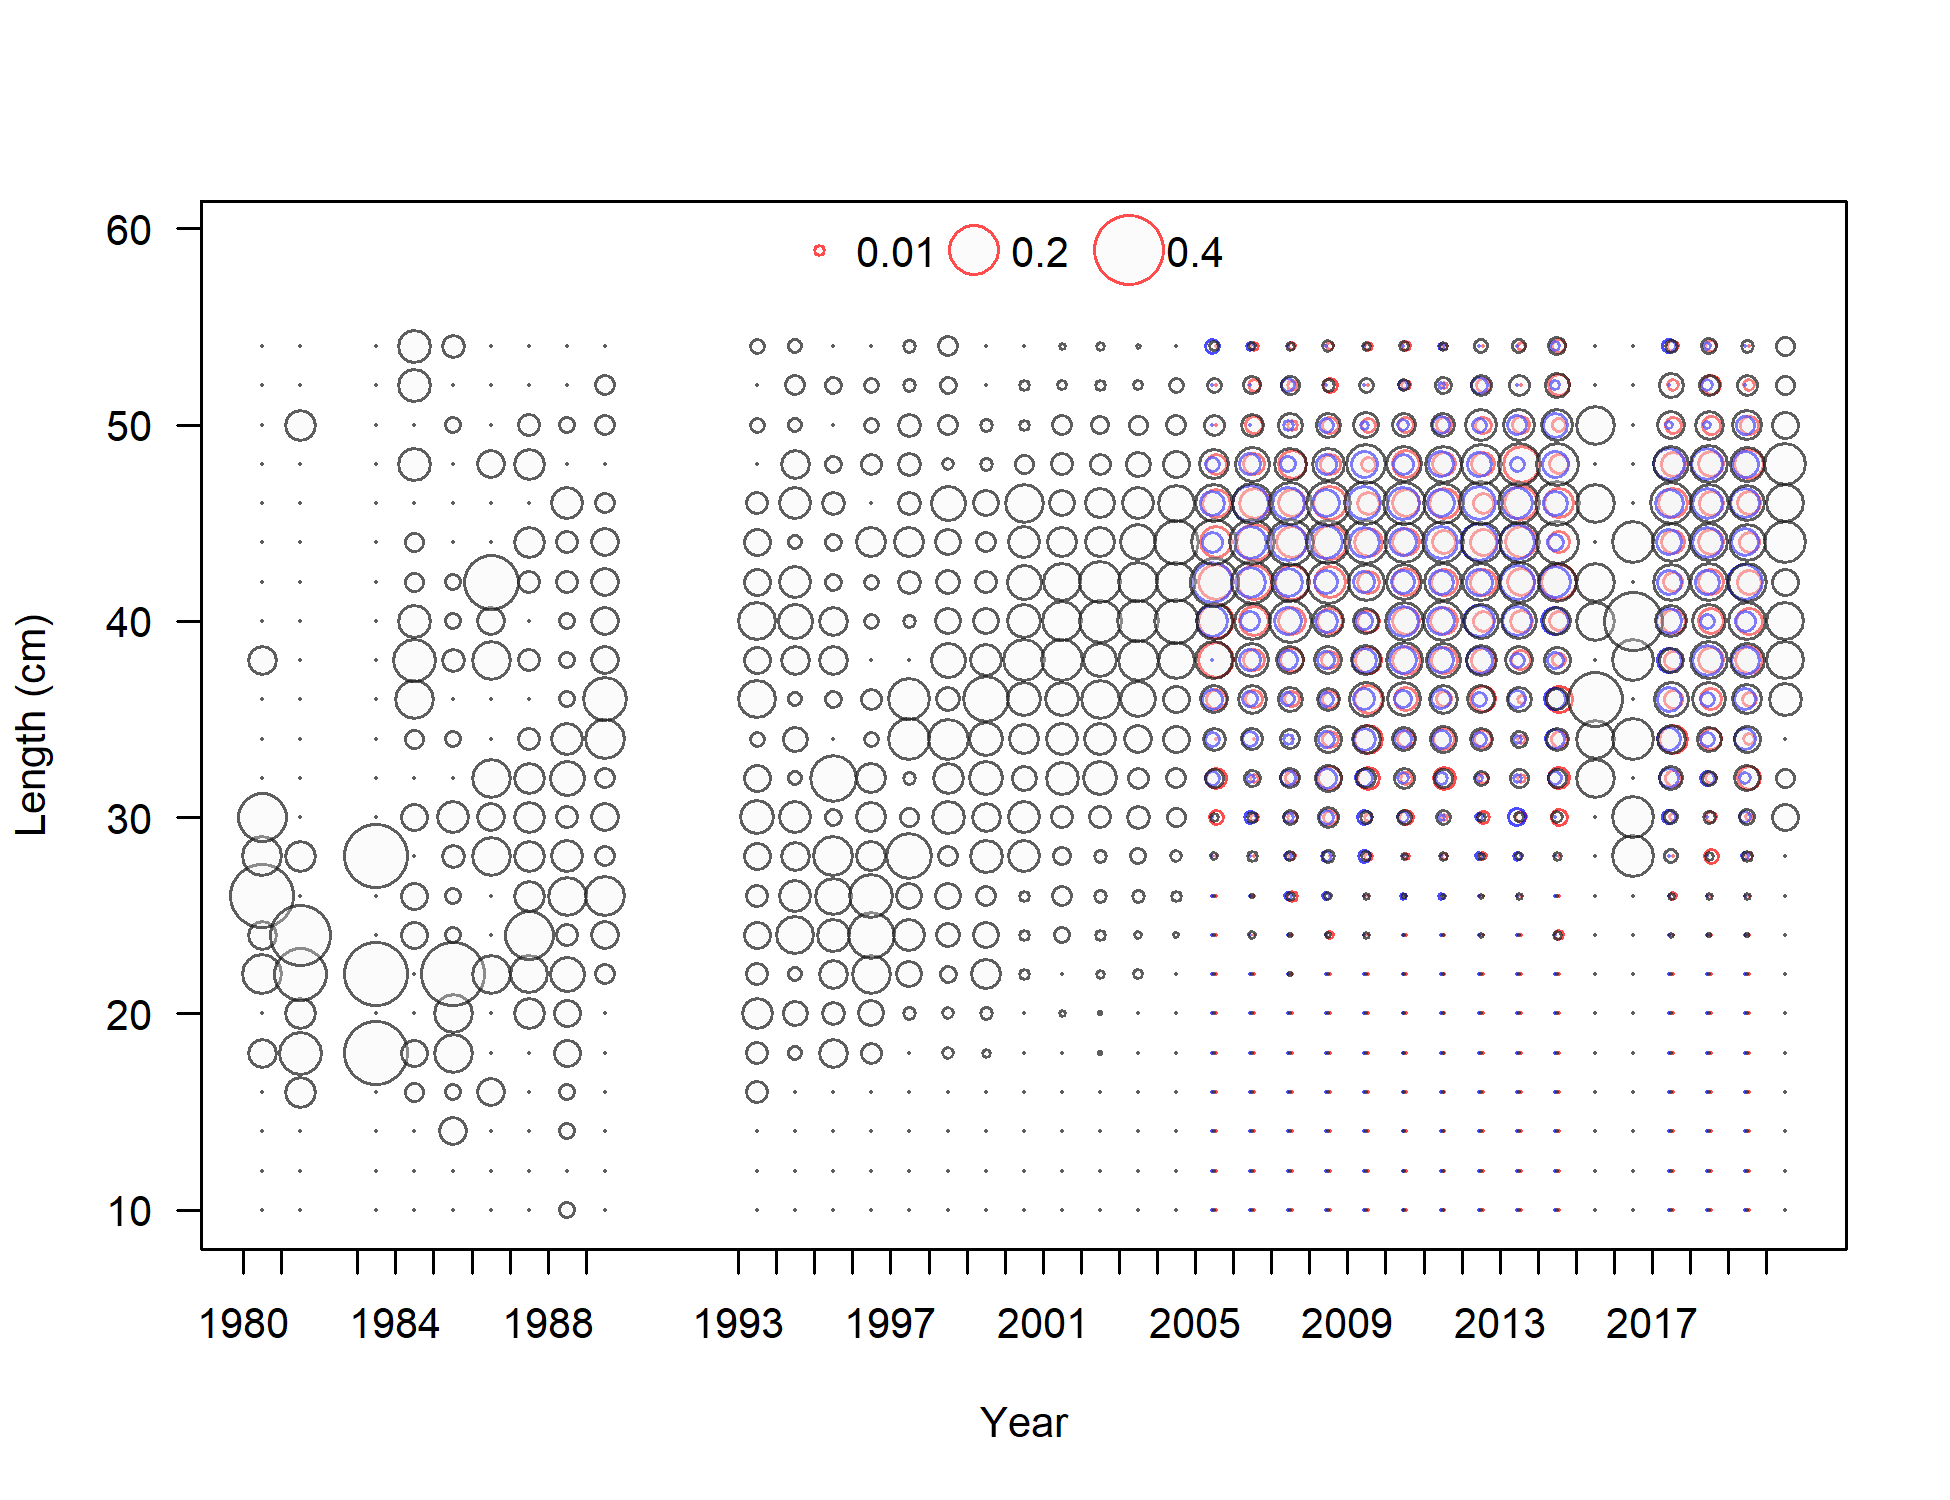
\includegraphics[width=1\textwidth,height=1\textheight]{C:/Users/Brian.Langseth/Desktop/ca/7_1_0_base/plots/comp_lendat_bubflt2mkt0_page3.png}
\caption{Length composition data from the recreational fleet.\label{fig:rec-len-data}}
\end{figure}

\tagmcend\tagstructend

\tagstructbegin{tag=Figure,alttext={Mean length for recreational fleet with 95 percent confidence intervals.}}\tagmcbegin{tag=Figure}

\begin{figure}
\centering
\includegraphics[width=1\textwidth,height=1\textheight]{C:/Users/Brian.Langseth/Desktop/ca/7_1_0_base/plots/comp_lendat_data_weighting_TA1.8_CA_Recreational.png}
\caption{Mean length for recreational fleet with 95 percent confidence intervals.\label{fig:mean-rec-len-data}}
\end{figure}

\tagmcend\tagstructend

\tagstructbegin{tag=Figure,alttext={Maturity as a function of  length.}}\tagmcbegin{tag=Figure}

\begin{figure}
\centering
\includegraphics[width=1\textwidth,height=1\textheight]{C:/Users/Brian.Langseth/Desktop/ca/7_1_0_base/plots/bio6_maturity.png}
\caption{Maturity as a function of length.\label{fig:maturity}}
\end{figure}

\tagmcend\tagstructend

\tagstructbegin{tag=Figure,alttext={Fecundity as a function of length.}}\tagmcbegin{tag=Figure}

\begin{figure}
\centering
\includegraphics[width=1\textwidth,height=1\textheight]{C:/Users/Brian.Langseth/Desktop/ca/7_1_0_base/plots/bio9_fecundity_len.png}
\caption{Fecundity as a function of length.\label{fig:fecundity}}
\end{figure}

\tagmcend\tagstructend

\tagstructbegin{tag=Figure,alttext={Observed sex-specific weight-at-length data from the individual sources with length and weight data, along with all sources combined with the estimated weight-at-length curves.}}\tagmcbegin{tag=Figure}

\begin{figure}
\centering
\includegraphics[width=1\textwidth,height=1\textheight]{//nwcfile/FRAM/Assessments/CurrentAssessments/DataModerate_2021/Quillback_Rockfish/data/output biology/plots/Length_Weight_by_Sex_ForReport.png}
\caption{Observed sex-specific weight-at-length data from the individual sources with length and weight data, along with all sources combined with the estimated weight-at-length curves.\label{fig:len-weight-survey}}
\end{figure}

\tagmcend\tagstructend

\tagstructbegin{tag=Figure,alttext={Weight-at-length relationship used in the model.}}\tagmcbegin{tag=Figure}

\begin{figure}
\centering
\includegraphics[width=1\textwidth,height=1\textheight]{C:/Users/Brian.Langseth/Desktop/ca/7_1_0_base/plots/bio5_weightatsize.png}
\caption{Weight-at-length relationship used in the model.\label{fig:len-weight}}
\end{figure}

\tagmcend\tagstructend

\tagstructbegin{tag=Figure,alttext={Observed sex-specific length-at-age data from the individual sources with length and age data, along with all sources combined with the estimated length-at-age curves.}}\tagmcbegin{tag=Figure}

\begin{figure}
\centering
\includegraphics[width=1\textwidth,height=1\textheight]{//nwcfile/FRAM/Assessments/CurrentAssessments/DataModerate_2021/Quillback_Rockfish/data/output biology/plots/Length_Age_by_Sex_ForReport.png}
\caption{Observed sex-specific length-at-age data from the individual sources with length and age data, along with all sources combined with the estimated length-at-age curves.\label{fig:len-age-data}}
\end{figure}

\tagmcend\tagstructend

\tagstructbegin{tag=Figure,alttext={Length at age in the beginning of the year in the ending year of the model.}}\tagmcbegin{tag=Figure}

\begin{figure}
\centering
\includegraphics[width=1\textwidth,height=1\textheight]{C:/Users/Brian.Langseth/Desktop/ca/7_1_0_base/plots/bio1_sizeatage.png}
\caption{Length at age in the beginning of the year in the ending year of the model.\label{fig:len-age-ss}}
\end{figure}

\tagmcend\tagstructend

\tagstructbegin{tag=Figure,alttext={Selectivity at length by fleet.}}\tagmcbegin{tag=Figure}

\begin{figure}
\centering
\includegraphics[width=1\textwidth,height=1\textheight]{C:/Users/Brian.Langseth/Desktop/ca/7_1_0_base/plots/sel01_multiple_fleets_length1.png}
\caption{Selectivity at length by fleet.\label{fig:selex}}
\end{figure}

\tagmcend\tagstructend

\tagstructbegin{tag=Figure,alttext={Estimated time series of age-0 recruits (1000s).}}\tagmcbegin{tag=Figure}

\begin{figure}
\centering
\includegraphics[width=1\textwidth,height=1\textheight]{C:/Users/Brian.Langseth/Desktop/ca/7_1_0_base/plots/ts11_Age-0_recruits_(1000s)_with_95_asymptotic_intervals.png}
\caption{Estimated time series of age-0 recruits (1000s).\label{fig:recruits}}
\end{figure}

\tagmcend\tagstructend

\tagstructbegin{tag=Figure,alttext={Estimated time series of recruitment deviations.}}\tagmcbegin{tag=Figure}

\begin{figure}
\centering
\includegraphics[width=1\textwidth,height=1\textheight]{C:/Users/Brian.Langseth/Desktop/ca/7_1_0_base/plots/recdevs2_withbars.png}
\caption{Estimated time series of recruitment deviations.\label{fig:rec-devs}}
\end{figure}

\tagmcend\tagstructend

\tagstructbegin{tag=Figure,alttext={Recruitment bias adjustment applied in the base model.}}\tagmcbegin{tag=Figure}

\begin{figure}
\centering
\includegraphics[width=1\textwidth,height=1\textheight]{C:/Users/Brian.Langseth/Desktop/ca/7_1_0_base/plots/recruit_fit_bias_adjust_forReport.png}
\caption{Recruitment bias adjustment applied in the base model.\label{fig:bias-adj}}
\end{figure}

\tagmcend\tagstructend

\tagstructbegin{tag=Figure,alttext={Pearson residuals for commercial fleet. Closed bubble are positive residuals (observed > expected) and open bubbles are negative residuals (observed < expected).}}\tagmcbegin{tag=Figure}

\begin{figure}
\centering
\includegraphics[width=1\textwidth,height=1\textheight]{C:/Users/Brian.Langseth/Desktop/ca/7_1_0_base/plots/comp_lenfit_residsflt1mkt0_page2.png}
\caption{Pearson residuals for commercial fleet. Closed bubble are positive residuals (observed \textgreater{} expected) and open bubbles are negative residuals (observed \textless{} expected).\label{fig:com-pearson}}
\end{figure}

\tagmcend\tagstructend

\tagstructbegin{tag=Figure,alttext={Model estimated mean length in cm (blue line) overlaid on mean length of commercial lengths (gray circles) with 95 percent confidence intervals (thick bars) based on current samples sizes. The thin bars indicate the confidence interval if Francis weighting were used instead.}}\tagmcbegin{tag=Figure}

\begin{figure}
\centering
\includegraphics[width=1\textwidth,height=1\textheight]{C:/Users/Brian.Langseth/Desktop/ca/7_1_0_base/plots/comp_lenfit_data_weighting_TA1.8_CA_Commercial.png}
\caption{Model estimated mean length in cm (blue line) overlaid on mean length of commercial lengths (gray circles) with 95 percent confidence intervals (thick bars) based on current samples sizes. The thin bars indicate the confidence interval if Francis weighting were used instead.\label{fig:com-mean-len-fit}}
\end{figure}

\tagmcend\tagstructend

\tagstructbegin{tag=Figure,alttext={Pearson residuals for recreational fleet. Closed bubble are positive residuals (observed > expected) and open bubbles are negative residuals (observed < expected).}}\tagmcbegin{tag=Figure}

\begin{figure}
\centering
\includegraphics[width=1\textwidth,height=1\textheight]{C:/Users/Brian.Langseth/Desktop/ca/7_1_0_base/plots/comp_lenfit_residsflt2mkt0_page3.png}
\caption{Pearson residuals for recreational fleet. Closed bubble are positive residuals (observed \textgreater{} expected) and open bubbles are negative residuals (observed \textless{} expected).\label{fig:rec-pearson}}
\end{figure}

\tagmcend\tagstructend

\tagstructbegin{tag=Figure,alttext={Model estimated mean length in cm (blue line) overlaid on mean length for recreational lengths (gray circles) with 95 percent confidence intervals (thick bars) based on current samples sizes. The thin bars indicate the confidence interval if Francis weighting were used instead.}}\tagmcbegin{tag=Figure}

\begin{figure}
\centering
\includegraphics[width=1\textwidth,height=1\textheight]{C:/Users/Brian.Langseth/Desktop/ca/7_1_0_base/plots/comp_lenfit_data_weighting_TA1.8_CA_Recreational.png}
\caption{Model estimated mean length in cm (blue line) overlaid on mean length for recreational lengths (gray circles) with 95 percent confidence intervals (thick bars) based on current samples sizes. The thin bars indicate the confidence interval if Francis weighting were used instead.\label{fig:rec-mean-len-fit}}
\end{figure}

\tagmcend\tagstructend

\tagstructbegin{tag=Figure,alttext={Aggregated length comps over all years.}}\tagmcbegin{tag=Figure}

\begin{figure}
\centering
\includegraphics[width=1\textwidth,height=1\textheight]{C:/Users/Brian.Langseth/Desktop/ca/7_1_0_base/plots/comp_lenfit__aggregated_across_time.png}
\caption{Aggregated length comps over all years.\label{fig:agg-len-fit}}
\end{figure}

\tagmcend\tagstructend

\tagstructbegin{tag=Figure,alttext={Estimated time series of spawning output.}}\tagmcbegin{tag=Figure}

\begin{figure}
\centering
\includegraphics[width=1\textwidth,height=1\textheight]{C:/Users/Brian.Langseth/Desktop/ca/7_1_0_base/plots/ts7_Spawning_output_with_95_asymptotic_intervals_intervals.png}
\caption{Estimated time series of spawning output.\label{fig:ssb}}
\end{figure}

\tagmcend\tagstructend

\tagstructbegin{tag=Figure,alttext={Estimated time series of total biomass.}}\tagmcbegin{tag=Figure}

\begin{figure}
\centering
\includegraphics[width=1\textwidth,height=1\textheight]{C:/Users/Brian.Langseth/Desktop/ca/7_1_0_base/plots/ts1_Total_biomass_(mt).png}
\caption{Estimated time series of total biomass.\label{fig:tot-bio}}
\end{figure}

\tagmcend\tagstructend

\tagstructbegin{tag=Figure,alttext={Estimated time series of relative spawning output.}}\tagmcbegin{tag=Figure}

\begin{figure}
\centering
\includegraphics[width=1\textwidth,height=1\textheight]{C:/Users/Brian.Langseth/Desktop/ca/7_1_0_base/plots/ts9_Relative_spawning_output_intervals.png}
\caption{Estimated time series of relative spawning output.\label{fig:depl}}
\end{figure}

\tagmcend\tagstructend

\tagstructbegin{tag=Figure,alttext={Stock-recruit curve. Point colors indicate year, with warmer colors indicating earlier years and cooler colors in showing later years.}}\tagmcbegin{tag=Figure}

\begin{figure}
\centering
\includegraphics[width=1\textwidth,height=1\textheight]{C:/Users/Brian.Langseth/Desktop/ca/7_1_0_base/plots/SR_curve.png}
\caption{Stock-recruit curve. Point colors indicate year, with warmer colors indicating earlier years and cooler colors in showing later years.\label{fig:bh-curve}}
\end{figure}

\tagmcend\tagstructend

\tagstructbegin{tag=Figure,alttext={Change in the negative log-likelihood across a range of ln(R0) values.}}\tagmcbegin{tag=Figure}

\begin{figure}
\centering
\includegraphics[width=1\textwidth,height=1\textheight]{C:/Users/Brian.Langseth/Desktop/ca/7_1_0_baseProfile_profile_SR_LN(R0)/piner_panel_SR_LN(R0).png}
\caption{Change in the negative log-likelihood across a range of ln(R0) values.\label{fig:r0-profile}}
\end{figure}

\tagmcend\tagstructend

\tagstructbegin{tag=Figure,alttext={Change in the estimate of spawning output across a range of ln(R0) values.}}\tagmcbegin{tag=Figure}

\begin{figure}
\centering
\includegraphics[width=1\textwidth,height=1\textheight]{C:/Users/Brian.Langseth/Desktop/ca/7_1_0_baseProfile_profile_SR_LN(R0)/SR_LN(R0)_trajectories_compare1_spawnbio.png}
\caption{Change in the estimate of spawning output across a range of ln(R0) values.\label{fig:r0-ssb}}
\end{figure}

\tagmcend\tagstructend

\tagstructbegin{tag=Figure,alttext={Change in the estimate of fraction unfished across a range of ln(R0) values.}}\tagmcbegin{tag=Figure}

\begin{figure}
\centering
\includegraphics[width=1\textwidth,height=1\textheight]{C:/Users/Brian.Langseth/Desktop/ca/7_1_0_baseProfile_profile_SR_LN(R0)/SR_LN(R0)_trajectories_compare3_Bratio.png}
\caption{Change in the estimate of fraction unfished across a range of ln(R0) values.\label{fig:r0-depl}}
\end{figure}

\tagmcend\tagstructend

\tagstructbegin{tag=Figure,alttext={Change in the negative log-likelihood across a range of steepness values.}}\tagmcbegin{tag=Figure}

\begin{figure}
\centering
\includegraphics[width=1\textwidth,height=1\textheight]{C:/Users/Brian.Langseth/Desktop/ca/7_1_0_baseProfile_profile_SR_BH_steep/piner_panel_SR_BH_steep.png}
\caption{Change in the negative log-likelihood across a range of steepness values.\label{fig:h-profile}}
\end{figure}

\tagmcend\tagstructend

\tagstructbegin{tag=Figure,alttext={Change in the estimate of spawning output across a range of steepness values.}}\tagmcbegin{tag=Figure}

\begin{figure}
\centering
\includegraphics[width=1\textwidth,height=1\textheight]{C:/Users/Brian.Langseth/Desktop/ca/7_1_0_baseProfile_profile_SR_BH_steep/SR_BH_steep_trajectories_compare1_spawnbio.png}
\caption{Change in the estimate of spawning output across a range of steepness values.\label{fig:h-ssb}}
\end{figure}

\tagmcend\tagstructend

\tagstructbegin{tag=Figure,alttext={Change in the estimate of fraction unfished across a range of steepness values.}}\tagmcbegin{tag=Figure}

\begin{figure}
\centering
\includegraphics[width=1\textwidth,height=1\textheight]{C:/Users/Brian.Langseth/Desktop/ca/7_1_0_baseProfile_profile_SR_BH_steep/SR_BH_steep_trajectories_compare3_Bratio.png}
\caption{Change in the estimate of fraction unfished across a range of steepness values.\label{fig:h-depl}}
\end{figure}

\tagmcend\tagstructend

\tagstructbegin{tag=Figure,alttext={Change in the negative log-likelihood across a range of natural mortality values.}}\tagmcbegin{tag=Figure}

\begin{figure}
\centering
\includegraphics[width=1\textwidth,height=1\textheight]{C:/Users/Brian.Langseth/Desktop/ca/7_1_0_baseProfile_profile_NatM_p_1_Fem_GP_1/piner_panel_NatM_p_1_Fem_GP_1.png}
\caption{Change in the negative log-likelihood across a range of natural mortality values.\label{fig:m-profile}}
\end{figure}

\tagmcend\tagstructend

\tagstructbegin{tag=Figure,alttext={Change in the estimate of spawning output across a range of natural mortality values.}}\tagmcbegin{tag=Figure}

\begin{figure}
\centering
\includegraphics[width=1\textwidth,height=1\textheight]{C:/Users/Brian.Langseth/Desktop/ca/7_1_0_baseProfile_profile_NatM_p_1_Fem_GP_1/NatM_p_1_Fem_GP_1_trajectories_compare1_spawnbio.png}
\caption{Change in the estimate of spawning output across a range of natural mortality values.\label{fig:m-ssb}}
\end{figure}

\tagmcend\tagstructend

\tagstructbegin{tag=Figure,alttext={Change in the estimate of fraction unfished across a range of natural mortality values.}}\tagmcbegin{tag=Figure}

\begin{figure}
\centering
\includegraphics[width=1\textwidth,height=1\textheight]{C:/Users/Brian.Langseth/Desktop/ca/7_1_0_baseProfile_profile_NatM_p_1_Fem_GP_1/NatM_p_1_Fem_GP_1_trajectories_compare3_Bratio.png}
\caption{Change in the estimate of fraction unfished across a range of natural mortality values.\label{fig:m-depl}}
\end{figure}

\tagmcend\tagstructend

\tagstructbegin{tag=Figure,alttext={Change in the negative log-likelihood across a range of maximum length values.}}\tagmcbegin{tag=Figure}

\begin{figure}
\centering
\includegraphics[width=1\textwidth,height=1\textheight]{C:/Users/Brian.Langseth/Desktop/ca/7_1_0_baseProfile_profile_L_at_Amax_Fem_GP_1/piner_panel_L_at_Amax_Fem_GP_1.png}
\caption{Change in the negative log-likelihood across a range of maximum length values.\label{fig:linf-profile}}
\end{figure}

\tagmcend\tagstructend

\tagstructbegin{tag=Figure,alttext={Change in the estimate of spawning output across a range of maximum length values.}}\tagmcbegin{tag=Figure}

\begin{figure}
\centering
\includegraphics[width=1\textwidth,height=1\textheight]{C:/Users/Brian.Langseth/Desktop/ca/7_1_0_baseProfile_profile_L_at_Amax_Fem_GP_1/L_at_Amax_Fem_GP_1_trajectories_compare1_spawnbio.png}
\caption{Change in the estimate of spawning output across a range of maximum length values.\label{fig:linf-ssb}}
\end{figure}

\tagmcend\tagstructend

\tagstructbegin{tag=Figure,alttext={Change in the estimate of fraction unfished across a range of maximum length values.}}\tagmcbegin{tag=Figure}

\begin{figure}
\centering
\includegraphics[width=1\textwidth,height=1\textheight]{C:/Users/Brian.Langseth/Desktop/ca/7_1_0_baseProfile_profile_L_at_Amax_Fem_GP_1/L_at_Amax_Fem_GP_1_trajectories_compare3_Bratio.png}
\caption{Change in the estimate of fraction unfished across a range of maximum length values.\label{fig:linf-depl}}
\end{figure}

\tagmcend\tagstructend

\tagstructbegin{tag=Figure,alttext={Change in the negative log-likelihood across a range of k values.}}\tagmcbegin{tag=Figure}

\begin{figure}
\centering
\includegraphics[width=1\textwidth,height=1\textheight]{C:/Users/Brian.Langseth/Desktop/ca/7_1_0_baseProfile_profile_VonBert_K_Fem_GP_1/piner_panel_VonBert_K_Fem_GP_1.png}
\caption{Change in the negative log-likelihood across a range of k values.\label{fig:k-profile}}
\end{figure}

\tagmcend\tagstructend

\tagstructbegin{tag=Figure,alttext={Change in the estimate of spawning output across a range of k values.}}\tagmcbegin{tag=Figure}

\begin{figure}
\centering
\includegraphics[width=1\textwidth,height=1\textheight]{C:/Users/Brian.Langseth/Desktop/ca/7_1_0_baseProfile_profile_VonBert_K_Fem_GP_1/VonBert_K_Fem_GP_1_trajectories_compare1_spawnbio.png}
\caption{Change in the estimate of spawning output across a range of k values.\label{fig:k-ssb}}
\end{figure}

\tagmcend\tagstructend

\tagstructbegin{tag=Figure,alttext={Change in the estimate of fraction unfished across a range of k values.}}\tagmcbegin{tag=Figure}

\begin{figure}
\centering
\includegraphics[width=1\textwidth,height=1\textheight]{C:/Users/Brian.Langseth/Desktop/ca/7_1_0_baseProfile_profile_VonBert_K_Fem_GP_1/VonBert_K_Fem_GP_1_trajectories_compare3_Bratio.png}
\caption{Change in the estimate of fraction unfished across a range of k values.\label{fig:k-depl}}
\end{figure}

\tagmcend\tagstructend

\tagstructbegin{tag=Figure,alttext={Change in the negative log-likelihood across a range of CV at maximum length values.}}\tagmcbegin{tag=Figure}

\begin{figure}
\centering
\includegraphics[width=1\textwidth,height=1\textheight]{C:/Users/Brian.Langseth/Desktop/ca/7_1_0_baseProfile_profile_CV_old_Fem_GP_1/piner_panel_CV_old_Fem_GP_1.png}
\caption{Change in the negative log-likelihood across a range of CV at maximum length values.\label{fig:cv2-profile}}
\end{figure}

\tagmcend\tagstructend

\tagstructbegin{tag=Figure,alttext={Change in the estimate of spawning output across a range of CV at maximum length values.}}\tagmcbegin{tag=Figure}

\begin{figure}
\centering
\includegraphics[width=1\textwidth,height=1\textheight]{C:/Users/Brian.Langseth/Desktop/ca/7_1_0_baseProfile_profile_CV_old_Fem_GP_1/CV_old_Fem_GP_1_trajectories_compare1_spawnbio.png}
\caption{Change in the estimate of spawning output across a range of CV at maximum length values.\label{fig:cv2-ssb}}
\end{figure}

\tagmcend\tagstructend

\tagstructbegin{tag=Figure,alttext={Change in the estimate of fraction unfished across a range of CV at maximum length values.}}\tagmcbegin{tag=Figure}

\begin{figure}
\centering
\includegraphics[width=1\textwidth,height=1\textheight]{C:/Users/Brian.Langseth/Desktop/ca/7_1_0_baseProfile_profile_CV_old_Fem_GP_1/CV_old_Fem_GP_1_trajectories_compare3_Bratio.png}
\caption{Change in the estimate of fraction unfished across a range of CV at maximum length values.\label{fig:cv2-depl}}
\end{figure}

\tagmcend\tagstructend

\tagstructbegin{tag=Figure,alttext={Change in the estimate of spawning output when the most recent 5 years of data are removed sequentially.}}\tagmcbegin{tag=Figure}

\begin{figure}
\centering
\includegraphics[width=1\textwidth,height=1\textheight]{C:/Users/Brian.Langseth/Desktop/ca/7_1_0_baseProfile_retro/compare2_spawnbio_uncertainty.png}
\caption{Change in the estimate of spawning output when the most recent 5 years of data are removed sequentially.\label{fig:retro-ssb}}
\end{figure}

\tagmcend\tagstructend

\tagstructbegin{tag=Figure,alttext={Change in the estimate of fraction unfished when the most recent 5 years of data are removed sequentially.}}\tagmcbegin{tag=Figure}

\begin{figure}
\centering
\includegraphics[width=1\textwidth,height=1\textheight]{C:/Users/Brian.Langseth/Desktop/ca/7_1_0_baseProfile_retro/compare4_Bratio_uncertainty.png}
\caption{Change in the estimate of fraction unfished when the most recent 5 years of data are removed sequentially.\label{fig:retro-depl}}
\end{figure}

\tagmcend\tagstructend

\tagstructbegin{tag=Figure,alttext={Change in the estimate of annual recruitment deviations when the most recent 5 years of data are removed sequentially.}}\tagmcbegin{tag=Figure}

\begin{figure}
\centering
\includegraphics[width=1\textwidth,height=1\textheight]{C:/Users/Brian.Langseth/Desktop/ca/7_1_0_baseProfile_retro/compare11_recdevs.png}
\caption{Change in the estimate of annual recruitment deviations when the most recent 5 years of data are removed sequentially.\label{fig:retro-recdevs}}
\end{figure}

\tagmcend\tagstructend

\tagstructbegin{tag=Figure,alttext={Change in estimated spawning output by sensitivity.}}\tagmcbegin{tag=Figure}

\begin{figure}
\centering
\includegraphics[width=1\textwidth,height=1\textheight]{C:/Users/Brian.Langseth/Desktop/ca/sensitivities/base.710_sensitivities_compare2_spawnbio_uncertainty.png}
\caption{Change in estimated spawning output by sensitivity.\label{fig:sens-ssb}}
\end{figure}

\tagmcend\tagstructend

\tagstructbegin{tag=Figure,alttext={Change in estimated fraction unfished by sensitivity.}}\tagmcbegin{tag=Figure}

\begin{figure}
\centering
\includegraphics[width=1\textwidth,height=1\textheight]{C:/Users/Brian.Langseth/Desktop/ca/sensitivities/base.710_sensitivities_compare4_Bratio_uncertainty.png}
\caption{Change in estimated fraction unfished by sensitivity.\label{fig:sens-depl}}
\end{figure}

\tagmcend\tagstructend

\tagstructbegin{tag=Figure,alttext={Change in estimated annual recruitment deviation.}}\tagmcbegin{tag=Figure}

\begin{figure}
\centering
\includegraphics[width=1\textwidth,height=1\textheight]{C:/Users/Brian.Langseth/Desktop/ca/sensitivities/base.710_sensitivities_compare12_recdevs_uncertainty.png}
\caption{Change in estimated annual recruitment deviation.\label{fig:sens-recdev}}
\end{figure}

\tagmcend\tagstructend

\tagstructbegin{tag=Figure,alttext={Estimated 1 - relative spawning ratio (SPR) by year.}}\tagmcbegin{tag=Figure}

\begin{figure}
\centering
\includegraphics[width=1\textwidth,height=1\textheight]{C:/Users/Brian.Langseth/Desktop/ca/7_1_0_base/plots/SPR2_minusSPRseries.png}
\caption{Estimated 1 - relative spawning ratio (SPR) by year.\label{fig:1-spr}}
\end{figure}

\tagmcend\tagstructend

\tagstructbegin{tag=Figure,alttext={Phase plot showing the fraction unfished versus fishing intensity for each year. Each point shows the spawning output relative to the unfished spawning output and the SPR ratio for each year. Lines through the final point show the 95 percent confidence intervals based on the asymptotic uncertainty for each dimension. The shaded ellipse is a 95 percent confidence region which accounts for the estimated correlations between the spawning output and SPR ratios..}}\tagmcbegin{tag=Figure}

\begin{figure}
\centering
\includegraphics[width=1\textwidth,height=1\textheight]{C:/Users/Brian.Langseth/Desktop/ca/7_1_0_base/plots/SPR4_phase.png}
\caption{Phase plot showing the fraction unfished versus fishing intensity for each year. Each point shows the spawning output relative to the unfished spawning output and the SPR ratio for each year. Lines through the final point show the 95 percent confidence intervals based on the asymptotic uncertainty for each dimension. The shaded ellipse is a 95 percent confidence region which accounts for the estimated correlations between the spawning output and SPR ratios..\label{fig:phase-plot}}
\end{figure}

\tagmcend\tagstructend

\tagstructbegin{tag=Figure,alttext={Equilibrium yield curve for the base case model. Values are based on the 2020 fishery selectivity and with steepness fixed at 0.72.}}\tagmcbegin{tag=Figure}

\begin{figure}
\centering
\includegraphics[width=1\textwidth,height=1\textheight]{C:/Users/Brian.Langseth/Desktop/ca/7_1_0_base/plots/yield2_yield_curve_with_refpoints.png}
\caption{Equilibrium yield curve for the base case model. Values are based on the 2020 fishery selectivity and with steepness fixed at 0.72.\label{fig:yield}}
\end{figure}

\tagmcend\tagstructend

\newpage

\clearpage

\tagstructbegin{tag=H1}\tagmcbegin{tag=H1}

\hypertarget{appendix}{%
\section{Appendix}\label{appendix}}

\leavevmode\tagmcend\tagstructend

\tagstructbegin{tag=H2}\tagmcbegin{tag=H2}

\hypertarget{append_a}{%
\subsection{Appendix A: California ROV Survey Data Informing Selectivity}\label{append_a}}

\leavevmode\tagmcend\tagstructend

\tagstructbegin{tag=P}\tagmcbegin{tag=P}

From 2013-2015, the CDFW in collaboration with Marine Applied Research and Exploration (MARE), conducted Remote Operated Vehicle (ROV) surveys along the full length of the California coastline inside MPAs and in reference sites outside for comparison. Density estimates were produced from the ratio of observed fish per unit area observed over the area of seafloor observed by the ROV in fish per meter squared. The percent relative density reflecting the proportion of the density observed in each depth bin was estimated relative to the sum of the density values in observed depths. A particular advantage of ROV data compared to other data sources is the accuracy of the depth of encounter of individual fish, providing useful information regarding selectivity of fishing gear relative to the depth distribution of fish observed by the ROV. Depth restrictions north of Point Conception varied from 20 to 40 fm for most of the last two decades. Densities were highest in the depths of 10 to 50 fm. Therefore, fish occur at depths greater than those that are open to fishing, indicating depth restrictions offer protection of quillback rockfish biomass (Table \ref{tab:ca-ROV}).

\leavevmode\tagmcend\tagstructend\par

\tagstructbegin{tag=P}\tagmcbegin{tag=P}

In addition, length frequency distributions by depth were determined from fish observed by the ROV based on visual approximations using the distance between paired lasers. While future efforts to increase the precision of length estimates include using stereo-camera data and programs estimating length from trigonometric calculations, the trends in approximate length distribution with depth still provides useful information. The length frequency distribution by depth is provided in Figure \ref{fig:ca-ROV}. In reviewing both the density by depth and length by depth relative to ontogenetic migration, the patterns may not reflect the smaller fish using shallow rocky reef as juveniles in less than 10 fm, and only reflect the density and composition in deeper depths where ontogenetic migration to deeper depths has already taken place for nearshore species and is not as apparent.

\leavevmode\tagmcend\tagstructend\par

\tagstructbegin{tag=P}\tagmcbegin{tag=P}

When examining the length composition data by depth inside and outside of MPAs north of Point Conception (Figure \ref{fig:ca-ROV}), no extreme differences in composition were observed, which is not surprising given the relatively recent implementation of MPAs north of Point Conception between 2007 and 2012. The MPAs make up 20-30\% of the rocky reef habitat in state waters within three miles of shore and are intended to preserve the larger individuals as biomass accumulates in MPAs over time. The combination of MPAs and RCAs restrict a larger portion of habitat to fishing (see {\tagstructbegin{tag=Link}\tagmcbegin{tag=Link}\protect\hyperlink{append_b}{Appendix B}\leavevmode\tagmcend\tagstructend} for details).

\leavevmode\tagmcend\tagstructend\par

\tagstructbegin{tag=P}\tagmcbegin{tag=P}

The percentage of fish in 5 cm size categories among 10 fm depths bins north of Point Conception did not show clear signs of increasing size with depth in greater than 10 fm in either region or protected vs.~reference sites (Figure \ref{fig:ca-ROV-percent}). This may be in part due to the fish having already moved from shallow kelp forest habitat where the ROV cannot operate to the adult depth distribution in greater than 10 fm by the time they are observed. Only in the shallower depth bins is there higher proportion of smaller individuals. This would indicate that selectivity may not be domed shaped as would be considered if the depth restrictions protected a larger proportion of adult biomass.

\leavevmode\tagmcend\tagstructend\par

\begingroup\fontsize{10}{12}\selectfont
\begingroup\fontsize{10}{12}\selectfont

\tagstructbegin{tag=Table}\tagmcbegin{tag=Table}
\begin{longtable}[t]{l>{\raggedright\arraybackslash}p{2.2cm}>{\raggedright\arraybackslash}p{2.2cm}>{\raggedright\arraybackslash}p{2.2cm}>{\raggedright\arraybackslash}p{2.2cm}}
\caption{\label{tab:ca-ROV}Counts of fish, areas surveyed by the ROV, density (fish/meter square) and percent relative density by 10 fm depth}\\
\toprule
Depth (fm) & Observed Area (m2) & Quillback Rockfish Observed & Quillback Rockfish Density (fish/m2) & Percent Relative Density\\
\midrule
\endfirsthead
\caption[]{\label{tab:ca-ROV}Counts of fish, areas surveyed by the ROV, density (fish/meter square) and percent relative density by 10 fm depth \textit{(continued)}}\\
\toprule
Depth (fm) & Observed Area (m2) & Quillback Rockfish Observed & Quillback Rockfish Density (fish/m2) & Percent Relative Density\\
\midrule
\endhead

\endfoot
\bottomrule
\endlastfoot
0-10 & 2905 & 0 & 0 & 0\\
10-20 & 124611 & 54 & 0.00043 & 0.17\\
20-30 & 106708 & 92 & 0.00086 & 0.34\\
30-40 & 86149 & 67 & 0.00078 & 0.3\\
40-50 & 49896 & 21 & 0.00042 & 0.16\\
50-60 & 16972 & 1 & 0.00006 & 0.02\\
60-70 & 1379 & 0 & 0 & 0\\
70-80 & 970 & 0 & 0 & 0\\
80-90 & 947 & 0 & 0 & 0\\
90-100 & 1257 & 0 & 0 & 0\\
100-110 & 608 & 0 & 0 & 0\\
110-120 & 696 & 0 & 0 & 0\\
120-130 & 415 & 0 & 0 & 0\\
130-140 & 777 & 0 & 0 & 0\\
140-150 & 1633 & 0 & 0 & 0\\
150-160 & 908 & 0 & 0 & 0\\
160-170 & 860 & 0 & 0 & 0\\
170-180 & 1268 & 0 & 0 & 0\\
180-190 & 912 & 0 & 0 & 0\\
190-200 & 735 & 0 & 0 & 0\\
200-210 & 604 & 0 & 0 & 0\\
210-220 & 167 & 0 & 0 & 0\\
220-230 & 54 & 0 & 0 & 0\\
230-240 & 100 & 0 & 0 & 0\\
Total & 401535 & 235 & - & -\\*
\end{longtable}
\leavevmode\tagmcend\tagstructend\par
\endgroup{}
\endgroup{}

\tagstructbegin{tag=Figure,alttext={Length frequency distribution in each 10 fm depth bin for quillback rockfish sampled by the ROV in reference locations open to fishing north of Point Conception (above) and State Marine Reserves prohibiting take (below).}}\tagmcbegin{tag=Figure}

\begin{figure}
\centering
\includegraphics[width=1\textwidth,height=1\textheight]{//nwcfile/FRAM/Assessments/CurrentAssessments/DataModerate_2021/Data_From_States/ca/quillback_rov_lengths.png}
\caption{Length frequency distribution in each 10 fm depth bin for quillback rockfish sampled by the ROV in reference locations open to fishing north of Point Conception (above) and State Marine Reserves prohibiting take (below).\label{fig:ca-ROV}}
\end{figure}

\tagmcend\tagstructend

\tagstructbegin{tag=Figure,alttext={Percent composition of quillback rockfish length frequency in 5 cm size classes for each 10 fm depth bin from ROV observations north of Point Conception in reference locations where retention is allowed (above) and in State Marine Reserves where retention is prohibited (below).}}\tagmcbegin{tag=Figure}

\begin{figure}
\centering
\includegraphics[width=1\textwidth,height=1\textheight]{//nwcfile/FRAM/Assessments/CurrentAssessments/DataModerate_2021/Data_From_States/ca/quillback_rov_barchart_length.png}
\caption{Percent composition of quillback rockfish length frequency in 5 cm size classes for each 10 fm depth bin from ROV observations north of Point Conception in reference locations where retention is allowed (above) and in State Marine Reserves where retention is prohibited (below).\label{fig:ca-ROV-percent}}
\end{figure}

\tagmcend\tagstructend

\clearpage

\tagstructbegin{tag=H2}\tagmcbegin{tag=H2}

\hypertarget{append_b}{%
\subsection{Appendix B: Percent Area Closed to Fishing in the RCAs and MPAs over time}\label{append_b}}

\leavevmode\tagmcend\tagstructend

\tagstructbegin{tag=P}\tagmcbegin{tag=P}

MPAs were instituted at various times from 2003 to 2012 as the area selection process was undertaken on a regional process. The existence of no take MPAs in some of the areas selected prior to expansion of the MPAs to encompass approximately 20-30\% of rocky reef habitat in state waters, duration of existence of new areas, degree of effort prior to protection or criteria for selection including productivity of the reef may have contributed to the current patterns in composition and density inside vs.~outside MPAs. As biomass accrues inside MPAs, accounting for protections through area-based assessment methods or effects on selectivity should be considered as fishery dependent data will only reflect the length composition and density outside the MPAs.

\leavevmode\tagmcend\tagstructend\par

\tagstructbegin{tag=P}\tagmcbegin{tag=P}

The percentage area closed to fishing in MPAs and Rockfish Conservation Areas (RCAs) north of Point Conception from 2001 to 2021 are shown in Table \ref{tab:ca-mpa}. The percentage closed to fishing provides a buffer against uncertainty through protection of a portion of the population. The percent area in MPAs prohibiting take by the recreational and commercial fisheries were included in the estimates of area closed to fishing from the first year in which the MPA was in place for a full calendar year. Areas closed to fishing prior to the implementation of the present MPA network were also accounted for. The RCAs for commercial and recreational fisheries were based on the deeper of the depth restrictions for the sectors to reflect only areas where take was prohibited for both. Where the RCA lines for the stock in question were not available, depth contours were used to approximate the percent of area closed. The presence of each type of closure in each assessment region and year was converted to tables of Boolean fields allowing GIS algorithms estimating the area open and closed to fishing. The distribution and area of rocky reef habitat was determined using the GIS layers rendering the results of the side scanning sonar from the California Seafloor Mapping Project to identify hard bottom at varying levels of resolution from two square meters to ten meters based on the depth surveyed due to cone width of the sonar. The area of rocky reef habitat closed to fishing within the depth distribution of the focal species was converted to a percentage of the total habitat.

\leavevmode\tagmcend\tagstructend\par

\begingroup\fontsize{10}{12}\selectfont
\begingroup\fontsize{10}{12}\selectfont

\tagstructbegin{tag=Table}\tagmcbegin{tag=Table}
\begin{longtable}[t]{l>{\raggedright\arraybackslash}p{2cm}>{\raggedright\arraybackslash}p{2cm}>{\raggedright\arraybackslash}p{2cm}}
\caption{\label{tab:ca-mpa}Percent of rocky reef habitat protected for quillback and copper rockfish north or Point Conception by MPAs and RCAs, and the total percent habitat open to fishing.}\\
\toprule
Year & Percent Habitat Protected by MPA & Percent Habitat Protected by RCA & Percent Habitat Open to Fishing\\
\midrule
\endfirsthead
\caption[]{\label{tab:ca-mpa}Percent of rocky reef habitat protected for quillback and copper rockfish north or Point Conception by MPAs and RCAs, and the total percent habitat open to fishing. \textit{(continued)}}\\
\toprule
Year & Percent Habitat Protected by MPA & Percent Habitat Protected by RCA & Percent Habitat Open to Fishing\\
\midrule
\endhead

\endfoot
\bottomrule
\endlastfoot
2001 & 4 & 0 & 96\\
2002 & 4 & 0 & 96\\
2003 & 4 & 38 & 59\\
2004 & 7 & 23 & 70\\
2005 & 7 & 29 & 64\\
2006 & 7 & 29 & 64\\
2007 & 7 & 27 & 66\\
2008 & 14 & 27 & 59\\
2009 & 14 & 27 & 59\\
2010 & 14 & 32 & 54\\
2011 & 21 & 30 & 49\\
2012 & 23 & 30 & 47\\
2013 & 26 & 30 & 44\\
2014 & 26 & 30 & 44\\
2015 & 26 & 27 & 47\\
2016 & 26 & 27 & 47\\
2017 & 26 & 16 & 58\\
2018 & 26 & 16 & 58\\
2019 & 26 & 13 & 61\\
2020 & 26 & 13 & 61\\
2021 & 26 & 6 & 68\\*
\end{longtable}
\leavevmode\tagmcend\tagstructend\par
\endgroup{}
\endgroup{}

\clearpage

\tagstructbegin{tag=H2}\tagmcbegin{tag=H2}

\hypertarget{append_c}{%
\subsection{Appendix C: Detailed Fit to Annual Length Composition Data}\label{append_c}}

\leavevmode\tagmcend\tagstructend

\tagstructbegin{tag=Figure,alttext={Length comps, whole catch, CA_Commercial (plot 1 of 2).<br><br>'N adj.' is the input sample size after data-weighting adjustment. N eff. is the calculated effective sample size used in the McAllister-Iannelli tuning method.}}\tagmcbegin{tag=Figure}

\begin{figure}
\centering
\includegraphics[width=1\textwidth,height=1\textheight]{C:/Users/Brian.Langseth/Desktop/ca/7_1_1_base_ghostCom/plots/comp_lenfit_flt1mkt0_page1.png}
\caption{Length comps, whole catch, CA\_Commercial (plot 1 of 2).`N adj.' is the input sample size after data-weighting adjustment. N eff. is the calculated effective sample size used in the McAllister-Iannelli tuning method.\label{fig:comp_lenfit_flt1mkt0_page1}}
\end{figure}

\tagmcend\tagstructend

\tagstructbegin{tag=Figure,alttext={Length comps, whole catch, CA_Commercial (plot 2 of 2).}}\tagmcbegin{tag=Figure}

\begin{figure}
\centering
\includegraphics[width=1\textwidth,height=1\textheight]{C:/Users/Brian.Langseth/Desktop/ca/7_1_1_base_ghostCom/plots/comp_lenfit_flt1mkt0_page2.png}
\caption{Length comps, whole catch, CA\_Commercial (plot 2 of 2).\label{fig:comp_lenfit_flt1mkt0_page2}}
\end{figure}

\tagmcend\tagstructend

\tagstructbegin{tag=Figure,alttext={Length comps, whole catch, CA_Recreational (plot 1 of 3).<br><br>'N adj.' is the input sample size after data-weighting adjustment. N eff. is the calculated effective sample size used in the McAllister-Iannelli tuning method.}}\tagmcbegin{tag=Figure}

\begin{figure}
\centering
\includegraphics[width=1\textwidth,height=1\textheight]{C:/Users/Brian.Langseth/Desktop/ca/7_1_1_base_ghostCom/plots/comp_lenfit_flt2mkt0_page1.png}
\caption{Length comps, whole catch, CA\_Recreational (plot 1 of 3).`N adj.' is the input sample size after data-weighting adjustment. N eff. is the calculated effective sample size used in the McAllister-Iannelli tuning method.\label{fig:comp_lenfit_flt2mkt0_page1}}
\end{figure}

\tagmcend\tagstructend

\tagstructbegin{tag=Figure,alttext={Length comps, whole catch, CA_Recreational (plot 2 of 3).}}\tagmcbegin{tag=Figure}

\begin{figure}
\centering
\includegraphics[width=1\textwidth,height=1\textheight]{C:/Users/Brian.Langseth/Desktop/ca/7_1_1_base_ghostCom/plots/comp_lenfit_flt2mkt0_page2.png}
\caption{Length comps, whole catch, CA\_Recreational (plot 2 of 3).\label{fig:comp_lenfit_flt2mkt0_page2}}
\end{figure}

\tagmcend\tagstructend

\tagstructbegin{tag=Figure,alttext={Length comps, whole catch, CA_Recreational (plot 3 of 3).}}\tagmcbegin{tag=Figure}

\begin{figure}
\centering
\includegraphics[width=1\textwidth,height=1\textheight]{C:/Users/Brian.Langseth/Desktop/ca/7_1_1_base_ghostCom/plots/comp_lenfit_flt2mkt0_page3.png}
\caption{Length comps, whole catch, CA\_Recreational (plot 3 of 3).\label{fig:comp_lenfit_flt2mkt0_page3}}
\end{figure}

\tagmcend\tagstructend

\tagstructbegin{tag=Figure,alttext={Ghost length comps, whole catch, CA_Commercial.<br><br>'N adj.' is the input sample size after data-weighting adjustment. N eff. is the calculated effective sample size used in the McAllister-Iannelli tuning method.}}\tagmcbegin{tag=Figure}

\begin{figure}
\centering
\includegraphics[width=1\textwidth,height=1\textheight]{C:/Users/Brian.Langseth/Desktop/ca/7_1_1_base_ghostCom/plots/comp_gstlenfit_flt1mkt0.png}
\caption{Ghost length comps, whole catch, CA\_Commercial.`N adj.' is the input sample size after data-weighting adjustment. N eff. is the calculated effective sample size used in the McAllister-Iannelli tuning method.\label{fig:comp_gstlenfit_flt1mkt0}}
\end{figure}

\tagmcend\tagstructend

\clearpage
\end{document}
